\documentclass[a4paper,12pt]{article}\usepackage[]{graphicx}\usepackage[]{color}
%% maxwidth is the original width if it is less than linewidth
%% otherwise use linewidth (to make sure the graphics do not exceed the margin)
\makeatletter
\def\maxwidth{ %
  \ifdim\Gin@nat@width>\linewidth
    \linewidth
  \else
    \Gin@nat@width
  \fi
}
\makeatother

\definecolor{fgcolor}{rgb}{0.345, 0.345, 0.345}
\newcommand{\hlnum}[1]{\textcolor[rgb]{0.686,0.059,0.569}{#1}}%
\newcommand{\hlstr}[1]{\textcolor[rgb]{0.192,0.494,0.8}{#1}}%
\newcommand{\hlcom}[1]{\textcolor[rgb]{0.678,0.584,0.686}{\textit{#1}}}%
\newcommand{\hlopt}[1]{\textcolor[rgb]{0,0,0}{#1}}%
\newcommand{\hlstd}[1]{\textcolor[rgb]{0.345,0.345,0.345}{#1}}%
\newcommand{\hlkwa}[1]{\textcolor[rgb]{0.161,0.373,0.58}{\textbf{#1}}}%
\newcommand{\hlkwb}[1]{\textcolor[rgb]{0.69,0.353,0.396}{#1}}%
\newcommand{\hlkwc}[1]{\textcolor[rgb]{0.333,0.667,0.333}{#1}}%
\newcommand{\hlkwd}[1]{\textcolor[rgb]{0.737,0.353,0.396}{\textbf{#1}}}%
\let\hlipl\hlkwb

\usepackage{framed}
\makeatletter
\newenvironment{kframe}{%
 \def\at@end@of@kframe{}%
 \ifinner\ifhmode%
  \def\at@end@of@kframe{\end{minipage}}%
  \begin{minipage}{\columnwidth}%
 \fi\fi%
 \def\FrameCommand##1{\hskip\@totalleftmargin \hskip-\fboxsep
 \colorbox{shadecolor}{##1}\hskip-\fboxsep
     % There is no \\@totalrightmargin, so:
     \hskip-\linewidth \hskip-\@totalleftmargin \hskip\columnwidth}%
 \MakeFramed {\advance\hsize-\width
   \@totalleftmargin\z@ \linewidth\hsize
   \@setminipage}}%
 {\par\unskip\endMakeFramed%
 \at@end@of@kframe}
\makeatother

\definecolor{shadecolor}{rgb}{.97, .97, .97}
\definecolor{messagecolor}{rgb}{0, 0, 0}
\definecolor{warningcolor}{rgb}{1, 0, 1}
\definecolor{errorcolor}{rgb}{1, 0, 0}
\newenvironment{knitrout}{}{} % an empty environment to be redefined in TeX

\usepackage{alltt}
\usepackage[margin=1in]{geometry}
\usepackage[utf8]{inputenc}
\usepackage{mathpazo}
%\usepackage{times}
\usepackage{booktabs}
\usepackage{multirow}
\usepackage{natbib}
\usepackage{amsmath}
\usepackage{setspace}
\usepackage[normalem]{ulem}
\usepackage{sectsty}
\subsectionfont{\normalfont\large\underline}
\usepackage{floatrow}
\floatsetup[figure]{capposition=top}
\floatsetup[table]{capposition=top}

\title{Measuring Subgroup Preferences in Conjoint Experiments\footnote{We thank Benjamin Lauderdale, Jamie Druckman, Yusaku Horiuchi, the editor, and anonymous reviewers for feedback on this manuscript.}}
\author{Thomas J. Leeper, Sara B. Hobolt, and James Tilley}
\IfFileExists{upquote.sty}{\usepackage{upquote}}{}
\begin{document}

\maketitle

{\abstract Conjoint analysis is an increasingly prominent tool for studying political preferences. The method powerfully disentangles patterns in respondents' favorability toward complex, multidimensional objects, such as political candidates or public policies. Most conjoint analyses rely upon a fully randomized conjoint design to generate average marginal component effects (AMCEs), which measure the degree to which a given value of a conjoint profile feature increases or decreases respondents' support for the overall profile relative to a baseline, averaging across all respondents and all other profile features. While the AMCE has a clear causal interpretation (about the \textit{effect} of features), most published conjoint analyses also use AMCEs to simply describe \textit{levels} of preferences or favorability, often including comparisons of AMCEs between subgroups of respondents. We show how this descriptive use of conditional AMCEs can be substantially misleading about the degree of agreement or disagreement between subgroups due the simple property that regression interactions are sensitive to the reference category used in the analysis. This leads to inferences about subgroup differences in preferences that have arbitrary sign, size, and significance. We demonstrate the problem using examples drawn from the published literature and provide suggestions for improved reporting and interpretation using two quantities of interest: the marginal mean and the omnibus F-test. Amidst the rapidly accelerating use of conjoint analyses, we highlight common pitfalls and offer advice for best practice in the analysis and presentation of conjoint experiments.}


















\clearpage


Amidst the dramatically increased use of experiments within political science \citep{Druckmanetal2006, Mutz2011}, conjoint experimental designs have recently become a prominent methodological tool in political science. While survey experiments have traditionally examined just one or two factors that might shape outcomes \citep[see, for reviews,][]{GainesKuklinskiQuirk2007, Sniderman2011}, conjoint designs allow researchers to study the independent effects on preferences of many features of complex, multidimensional objects such as political candidates \citep{Campbelletal2016, TeeleKallaRosenbluth2018}, immigrant admissions \citep{HainmuellerHopkins2015, BansakHainmuellerHangartner2016, WrightLevyCitrin2016}, or public policies \citep{GallegoMarx2017, Hankinson2018}. Factorial designs of this sort have a long history but the driving force behind this use of conjoint analysis has been the introduction by \citet{HainmuellerHopkinsYamamoto2014} of a small-sample, fully randomized conjoint design and an associated analytic approach that emphasizes a single quantity of interest: namely, the average marginal component effect (AMCE). By capturing the multidimensionality of target objects, the randomized conjoint design breaks any explicit or implicit confounding between features of these objects, giving the AMCE a clear causal interpretation: the degree to which a given value of a feature increases or decreases respondents' favorability toward a packaged conjoint profile relative to a baseline. 

While randomization of profile features gives the AMCE a causal interpretation, most published conjoint analyses in political science use AMCEs not only for \textit{causal} purposes (interpreting AMCEs as effect sizes), but also for \textit{descriptive} purposes: that is, to map levels of favorability toward a multidimensional object across its various features.\footnote{See \citet{Shmueli2010} for an elaboration on the distinctions between explanatory (causal) modelling, descriptive modelling, and predictive modelling.} In this sense, conjoints are often applied like list experiments, using randomization to measure a sample's preferences over something difficult to measure with direct questioning. A positive (negative) AMCE for a given feature can be read as a descriptive measure of high (low) favorability toward profiles with that feature. Though the quantity is causal, it is often read descriptively.

This is particularly the case when researchers engage in subgroup analyses of conjoint experiments in search of preference heterogeneity. Such exercises are an increasingly common feature of experimental analysis \citep{GreenKern2012, RatkovicTingley2017, GrimmerMessingWestwood2017, EgamiImai2018}. For example, \citet{HainmuellerHopkinsYamamoto2014} perform a subgroup analysis on their original immigration experiment in which they perform a median split on a measure of ethnocentrism and then compare AMCEs for the two subgroups. Similarly, \citet{BansakHainmuellerHangartner2016} compare preferences toward immigrants across number of binary respondent characteristics: age, education, left-right ideology, and income. In a different domain, \citet{BallardRosaMartinScheve2016} compare preferences over tax policies across a number of subgroups defined by demographics and political orientations. \citet{BechtelScheve2013} compare AMCEs on climate agreements across four different countries, and across subgroups of respondents. \citet{TeeleKallaRosenbluth2018} compare AMCEs for features of male and female political candidates among male and female respondents. Most of these comparisons are visual or informal. But some involve explicit estimation of the subgroup difference, such as when \citet{KirklandCoppock2017} compare conditional AMCEs across hypothetical partisan and nonpartisan elections. Interpretation of subgroup AMCEs thus involves an implied quantity of interest: the \textit{difference} between two conditional AMCEs.

What is not necessarily obvious in such analyses is that differences-in-preferences (that is to say, the difference in degree of favorability toward profiles containing a given feature) are not directly reflected in subgroup differences-in-AMCEs. A difference in effect sizes is distinct from a difference in the preferences so affected. We show that a difference in two (or more) subgroups' favorability toward a conojoint feature --- like a difference in willingness to support a Syrian immigrant between high and low ethnocentrism respondents --- is only reflected in the difference-in-AMCEs in very rare circumstances. As such, no information about the similarity of the subgroups' preferences is provided by comparisons of subgroup AMCEs, yet such comparisons are commonly made in practice.

As we will show, where preferences in subgroups toward the experimental reference category are similar, the difference-in-AMCEs conveys preferences reasonably well but where preferences between subgroups diverge in the reference category, the difference-in-AMCEs is a misleading representation of underlying patterns of favorability. Given most published conjoint studies appear to report results based upon reference categories chosen for \textit{substantive} reasons about the nature or meaning of the levels rather than the configuration of preferences revealed in the experiment, difference-in-AMCEs should not be assumed to be interpretable as differences in subgroup preferences.\footnote{For example, in a comparison of subgroup effects for Democrats and Republicans, Republicans might display a smaller effect because their preferences in the reference category are already very positive, such that a large positive effect for Democrats occurs despite Democrats being less supportive than Republicans in either experimental condition.} The root of this error is likely familiar to many researchers: it is simply a matter of regression specification for models involving interactions between categorical regressors. \citet{EgamiImai2018}, for example, provide an extensive discussion of the implications of this property for interpreting causal interactions between randomized features of conjoint profiles. The state of the published literature would suggest the problem remains non-obvious when applied to descriptive analysis of subgroups in conjoint designs.

In what follows, we demonstrate the challenges of conjoint analysis and remind readers of how reference category choice for profile features creates problems for comparing conditional AMCEs across respondent subgroups. We show how the use of an arbitrary reference category means the size, direction, and statistical significance of differences-in-AMCEs have little relationship to the underlying degree of favorability of the subgroups toward profiles with particular features; reference category choices can make similar preferences look dissimilar and dissimilar preferences look similar. We demonstrate this with examples drawn from the published political science literature (namely experiments by \citealt{HainmuellerHopkinsYamamoto2014, BechtelScheve2013, TeeleKallaRosenbluth2018}). The paper then provides suggestions for improved conjoint reporting and interpretation based around two quantities of interest drawn from the factorial experimentation literature: (a) unadjusted marginal means, a quantity measuring favorability toward a given feature, and (b) an omnibus F-test, measuring differences therein. Software for the R programming language to support our findings --- and that can be used to examine sensitivity of conjoint analysis to reference category selection, calculate AMCEs and marginal means, perform subgroup analyses, and test for subgroup differences in any conjoint experiment --- is demonstrated throughout. We conclude with advice for best practices in the analysis and presentation of conjoint results.

\section*{Quantities of Interest in Conjoint Experiments}\label{sec:quantities}

Conjoint analysis serves two purposes. One is to assess causal effects. Another is preference description.\footnote{Here we use ``preference'' as \citet{HainmuellerHopkinsYamamoto2014} do: that is, as a statement of \textit{favorability} or \textit{support} for a profile, not the more narrow economic definition of a strict rank ordering of objects by favorability.} In causal inference, fully randomized conjoints provide a design and analytic approach that allows researchers to understand the causal effect of a given feature on overall support for a multidimensional object, averaging across other features of the object included in the design. Such inferences can be thought of as statements of the form: ``shifting an immigrant's country of origin from India to Poland increases favorability by X percentage points.'' In descriptive inference, conjoints provide information about both (a) the \textit{absolute} favorability of respondents toward objects with particular features or combinations of features, and (b) the \textit{relative} favorability of respondents toward an object with alternative combinations of features. Such inferences can be thought of as statements of the form ``Polish immigrants are preferred by X\% of respondents'' or ``Polish immigrants are more supported than Mexican immigrants, by X percentage points.'' Thus both causal and descriptive interpretations of conjoints are based upon the distribution of preferences across profile features and differences in preferences across alternative feature combinations.

Analytically, a fully randomized conjoint design without constraints between profile features is simply a full-factorial experiment (with some cells possibly, albeit randomly, left unobserved). All quantities of interest relevant to the analysis of conjoint designs therefore derive from combinations of cell means, marginal means, and the grand mean, as in the traditional analysis of factorial experiments. In a forced choice conjoint design, the \textit{grand mean} is by definition 0.5 (i.e., 50\% of all profiles shown are chosen and 50\% are not chosen). \textit{Cell means} are the mean outcome for each particular combination of feature levels. In the full-factorial design discussed by \citet{HainmuellerHopkinsYamamoto2014} and now widely used in political science, many or perhaps most cell means are unobserved. For example, in their candidate choice experiment, there are $2*6*6*6*2*6*6*6 = 186,624$ cell means but only 3,466 observations so about 98\% of cell means are unobserved. While this would be problematic for attempting to infer pairwise comparisons between cells, conjoint analysts mostly focus on the marginal effects of each feature rather than more complex interactions. Appendix \ref{app:quantities} provides detailed notation and elaborations of these definitions of quantities of interest.

In fully randomized designs, the average marginal component effects (AMCEs) are simply marginal effects of changing one feature level to another, all else constant. AMCEs therefore depend only upon \textit{marginal means}: that is the column and row mean outcomes for each feature level averaging across all other features. A marginal mean describes the level of favorability toward profiles that have a particular feature level, ignoring all other features. For example, in the common forced-choice design with two alternatives, marginal means have a direct interpretation as probabilities: a marginal mean of 0 indicates respondents select profiles with that feature level with probability $P(Y=1|X=x) = 0$ while a marginal mean of 1 indicates respondents select profiles with that feature level with probability $P(Y=1|X=x)=1$, where $Y$ is a binary outcome and $X$ is a vector of profile features.\footnote{It is not possible for the marginal mean to equal zero or one if pairs of profiles shown together are allowed to have the same level of a given feature (for example, both immigrants are from Germany). Instead, the marginal mean can range from the probability of co-occurrence to 1 minus that probability. If there are five levels of a feature, each shown with equal probability, then the probability of co-occurrence is $\frac{1}{5}*\frac{1}{5} = 0.04$ such that the marginal mean can take values in the range $(0.04,0.96)$. If the design is constrained so that features cannot be the same for both immigrants, then the marginal means fully range from zero to one. This constraint on the range of the marginal means also constrains the range of AMCEs. Notably, many conjoints provide features with only two levels, such as the male-versus-female candidate feature examined by \citet{TeeleKallaRosenbluth2018} or \citet{HainmuellerHopkinsYamamoto2014} in their conjoints on candidate choice. In such cases, the probability of co-occurrence is $\frac{1}{2}*\frac{1}{2} = 0.25$ bounding the AMCE for female (as opposed to male) candidates to the range $(-0.5, 0.5)$ if both candidates can have the same sex. Caution is therefore needed in comparing the relative size of features with few levels to features with many levels given that effects have different bounds.} With rating scale outcomes, marginal means can vary arbitrarily along the outcome scale used.

\begin{knitrout}
\definecolor{shadecolor}{rgb}{0.969, 0.969, 0.969}\color{fgcolor}\begin{figure}
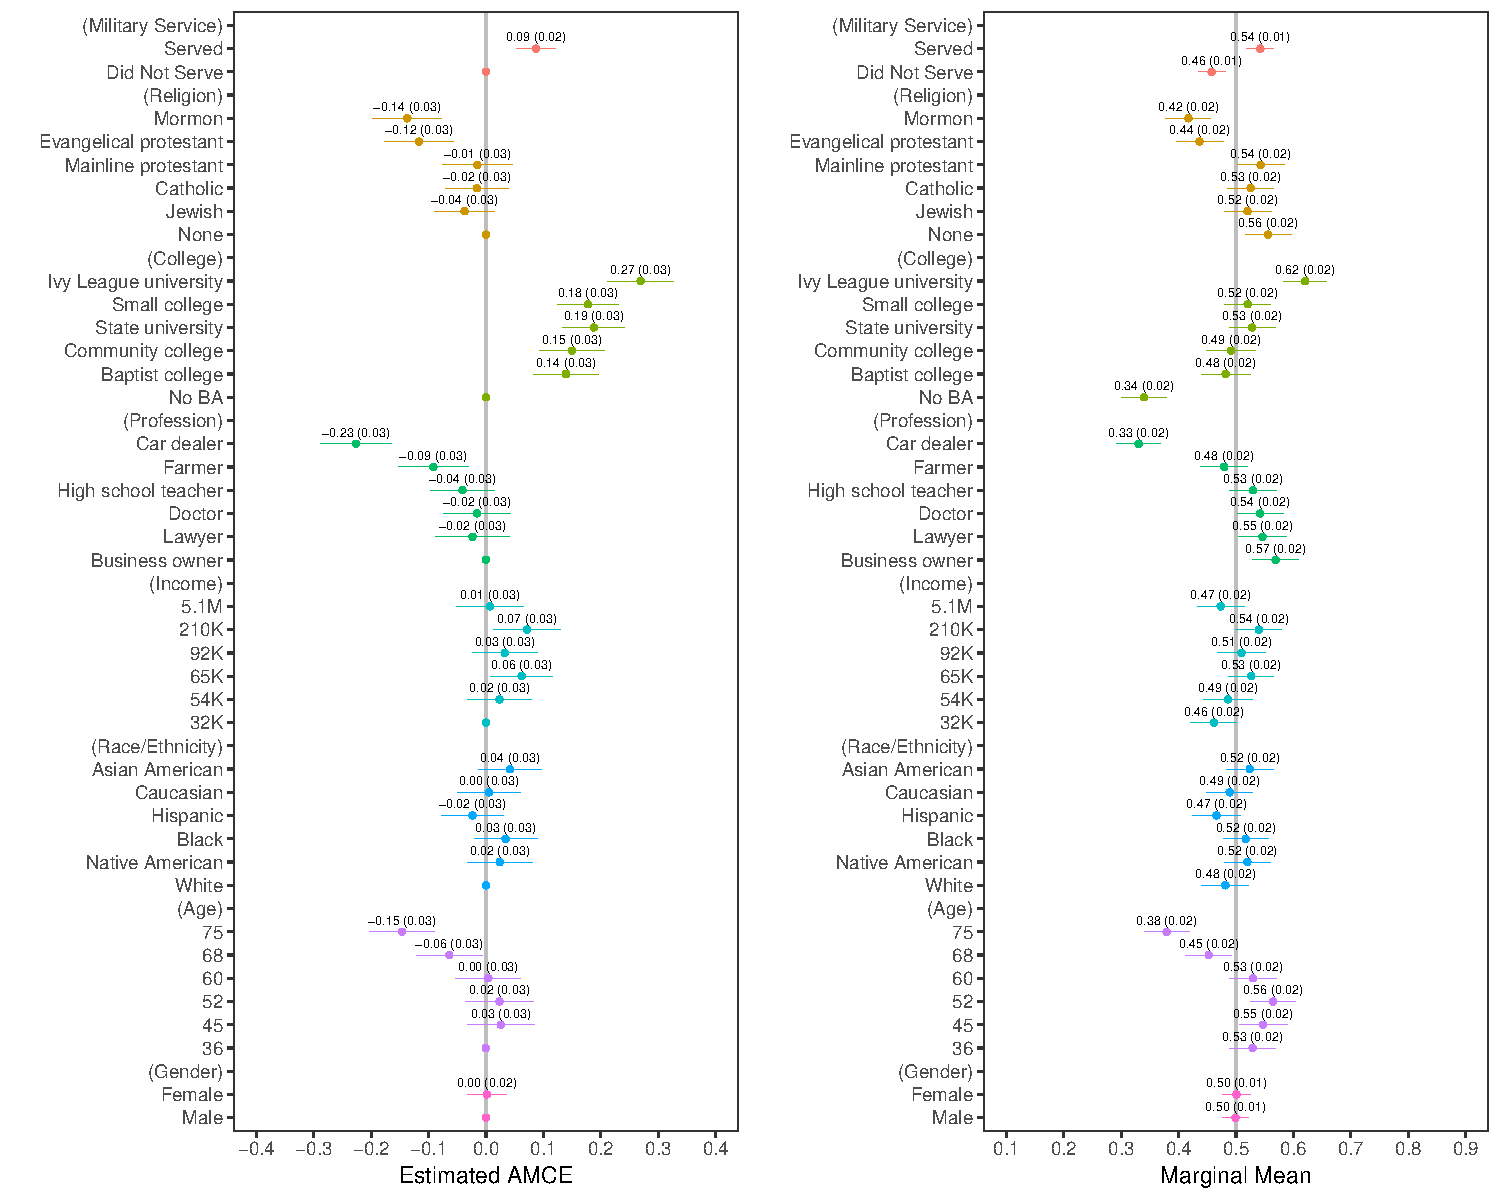
\includegraphics[width=\maxwidth]{figure/hainmueller_candidate_replication-1} \caption[Replication of Hainmueller et al]{Replication of Hainmueller et al. (2014) Candidate Experiment using AMCEs and MMs}\label{fig:hainmueller_candidate_replication}
\end{figure}


\end{knitrout}

Because levels of features are randomly assigned, pairwise differences between two marginal means for a given feature (e.g., between candidates who are male versus female) have a direct causal interpretation. For fully randomized designs, the AMCE proposed by \citet{HainmuellerHopkinsYamamoto2014} is equivalent to the average marginal effect of each feature level for a model where each feature is converted into a matrix of indicator variables with one level left out as a reference category. This is no different from any other regression context wherein one level of any categorical variable must be omitted from the design matrix in order to avoid perfect multicollinearity.\footnote{In designs that entail constraints between profile features, the average marginal effect is a weighted average of effects across each combination of the constrained features where the weights on the effects are arbitrary but typically uniform. We ignore this distinction in the remainder of this article, as all of our results apply equally to fully randomized and to constrained designs.} This close relationship between AMCEs and marginal means is visible in Figure \ref{fig:hainmueller_candidate_replication} which presents a replication of the AMCE-based analysis of the Hainmueller et al. candidate experiment (left panel) and an analogous examination of the results using marginal means (right panel). Note, in particular, how marginal means convey information about the preferences of respondents for all feature levels while AMCEs definitionally restrict the AMCE for the reference category to zero (or undefined). For example, the AMCE for a candidate serving in the military is 0.09 (or a 9-percentage point) increase in favorability, reflecting marginal means for serving and non-serving candidates of 0.46 and 0.54, respectively. Similarly, the zero effect size for candidate gender reflects identical marginal means for male and female candidates (0.50 in each case). AMCEs in fully randomized designs are simply differences between marginal means at each feature level and the marginal mean in the reference category, ignoring other features.

The AMCE is often described as an estimate of the relative favorability of profiles with counterfactual levels of a feature. For example, \citet{TeeleKallaRosenbluth2018} summarize their conjoint on public support ``female candidates are favored [over men] by 7.3 percentage points'' (6). Similarly, \citet{HainmuellerHopkinsYamamoto2014} describe some of the results of conjoint on preferences toward political candidates:

\begin{quote}
We also see a bias against Mormon candidates, whose estimated level of support is 0.06 (SE = 0.03) lower when compared to a baseline candidate with no stated religion. Support for Evangelical Protestants is also 0.04 percentage points lower (SE = 0.02) than the baseline. (19)
\end{quote}

\noindent These examples make clear that despite the \textit{causal} inference potentially provided by the AMCE, the quantity of interest is frequently used to provide a characterization of a preferences that has a distinctly descriptive flavor about the relative \textit{levels} of support across profiles and also across subgroups of respondents. Indeed, this style of description is widespread in conjoint analyses. This use of conjoints to provide descriptive inferences about patterns of preferences is important because AMCEs are defined as \textit{relative} quantities, requiring that patterns of preferences are expressed against a baseline, reference category for each conjoint feature. A positive (negative) AMCE is read as higher (lower) favorability but it is only higher (lower) relative to whatever category serves as the baseline. For example, in the \citeauthor{HainmuellerHopkinsYamamoto2014} candidate example, choosing a non-religious candidate as a baseline means the AMCEs in the candidate experiment are all expressed relative to this non-religious baseline; the difference (if any) between other pairs of marginal means (e.g., evaluations of Mormon and Evangelical candidates) is not obvious. Relatedly, the negative direction (and the size) of the AMCEs for Mormon and Evangelical candidates would be different if the least-liked category (Mormon candidates) were the reference group. In that case, the AMCE for Evangelicals would be small and positive and the AMCEs for all other categories (including the presented reference category, ``none'') would be large and positive. More trivially, \citet{TeeleKallaRosenbluth2018} describe their comparisons about public preferences for female candidates relative to male candidates, but could have equivalent described patterns of equal size but opposite sign comparing preferences over male relative to female candidates.

\begin{knitrout}
\definecolor{shadecolor}{rgb}{0.969, 0.969, 0.969}\color{fgcolor}\begin{figure}
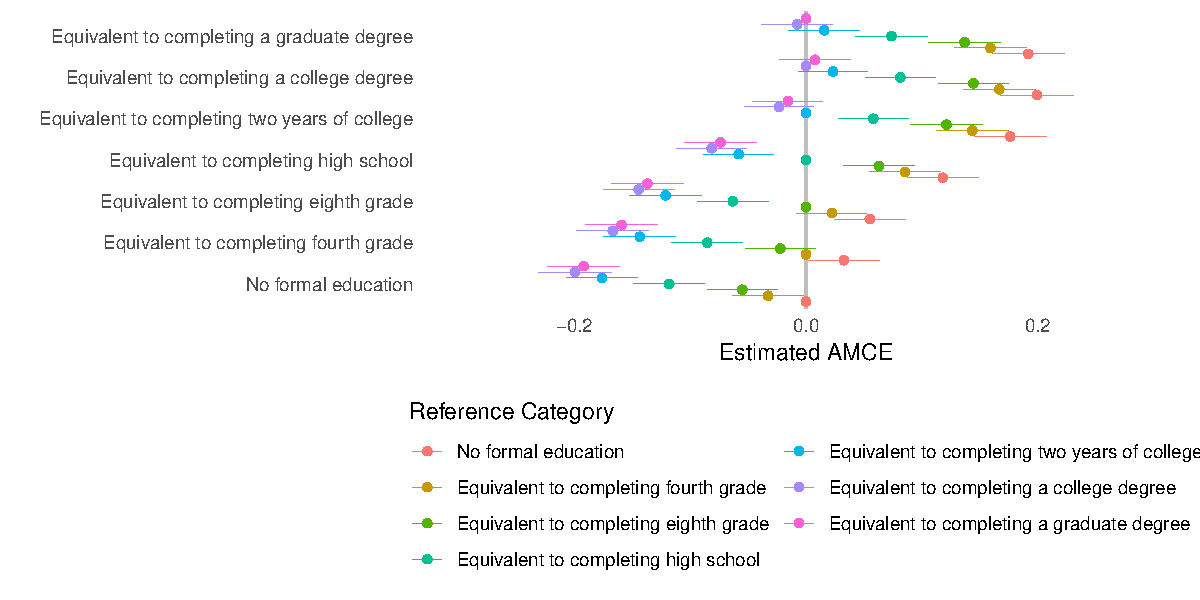
\includegraphics[width=\maxwidth]{figure/reference_category-1} \caption[Estimated AMCEs for Levels of the `Education' Feature for Each Possible Reference Category from Hainmueller et al.'s (2014) Immigration Experiment]{Estimated AMCEs for Levels of the `Education' Feature for Each Possible Reference Category from Hainmueller et al.'s (2014) Immigration Experiment}\label{fig:reference_category}
\end{figure}


\end{knitrout}

Though seemingly arbitrary, the choice of reference category for estimating AMCEs can be quite consequential.\footnote{Since this manuscript has been under review, we have been made aware of one working paper by \citet{ClaytonFerwerdaHoriuchi2018}, on the topic of immigration preferences, that correctly notes the need to address the arbitrary reference category in order to compare subgroup preferences.} For example, in \citeauthor{HainmuellerHopkinsYamamoto2014}'s candidate experiment (again, see \ref{fig:hainmueller_candidate_replication}), the least liked education level (``no formal education'') is chosen as a reference category, but the authors could have presented the results using any of the categories as the baseline. Figure \ref{fig:reference_category} shows how the estimated AMCEs for each level of the education feature would have differed depending on that choice. Selecting a reference category that receives middling support (i.e., more favorability than some other feature levels but less favorability than others), makes some AMCEs positive and others negative but all AMCEs can be made positive (or negative) simply by choosing a different baseline. The results would be numerically equivalent --- the alternative linear models used to the estimate the AMCEs have a mathematical equivalence --- but the choice has sizeable consequences for the interpretation of conjoint analyses, as we discuss below.\footnote{In \textit{constrained} conjoint designs, the choice of reference category is even more important. Consider, for example, the design of \citeauthor{HainmuellerHopkinsYamamoto2014}'s immigration experiment, which constrains the ``Country of Origin`` feature so that levels `India,' `Germany,' `France,' `Mexico,' `Philippines,' and `Poland' cannot co-occur with the `Escape Persecution' level of the ``Reason for Application'' feature. Consequently, the AMCE for the ``Escape Persecution'' level (relative to the  ``Reunite with family'' reference category) is only defined for the subset of the design involving countries `China,' `Sudan,' `Somalia,' and `Iraq.' The AMCEs for those four countries (relative to India as a baseline) marginalize across all reasons for application, but the AMCEs for the first six countries marginalize only across the latter two reasons. Thus the interpretation of AMCEs --- and the basic ability to estimate them in constrained designs --- depends entirely upon the selection of a reference category where all feature levels can co-occur. In a design where \textit{all} features are constrained, then AMCEs are undefined for the design as a whole and only estimable for subsets of the design that are \textit{conditionally} unconstrained.}

%To demonstrate this, Figure \ref{fig:reference_category} shows the estimated AMCEs for the country of origin feature from \citeauthor{HainmuellerHopkinsYamamoto2014}'s immigration experiment, with the analysis repeated ten times each time using a different country as the reference category. For example, the top-most set of points and error bars convey the AMCE for Iraq from each of these analyses. When Iraq is the reference category, its AMCE is undefined. When any other country is chosen as a reference category, the AMCE for Iraq is negative because respondents are more negative toward Iraqi immigrants than they are toward those of other countries. Similarly, the bottom set of points and error bars reflects the estimated AMCEs for Germany. When Germany is the reference category, its AMCE is undefined but when any other country is used as the reference category, its AMCE is positive.

%These cases are therefore not \textit{directionally} sensitive to the choice of reference category but of course the point estimates vary considerably. But the estimated AMCE of countries who are neither strongly disliked or strongly favored by respondents are highly sensitive to choice of reference category. Consider, for example, the estimated AMCEs for China (the four set of points from the top). When highly disliked countries are chosen as the reference category (like Somalia, Sudan, or Iraq), the AMCE for China is positive; when highly favored countries are chosen (like Germany, Poland, or the Philippines), the AMCE for China is negative.

\section*{Consequences of Arbitrary Reference Category Choice}\label{sec:challenges}

Given the need to choose a reference category for every feature in order to estimate AMCEs, an important question is: how do researchers decide which of tens of thousands of possible experimental cells should be selected as the reference category? Examining recently published conjoint analyses, it appears that the choice of reference category is either arbitrary or based upon substantive intuition about the meaning of feature levels. For example, \citet{HainmuellerHopkinsYamamoto2014} choose female immigrants as a baseline in their immigration experiment, thus providing an estimate of the AMCE of being male, while \citet{TeeleKallaRosenbluth2018} choose male candidates as a baseline in their conjoint, thus providing an estimate of the AMCE of being female. The choice is seemingly innocuous. Sometimes choices of reference category appear to be driven by substantive knowledge: on language skills of immigrants in their immigration experiment, \citet{HainmuellerHopkinsYamamoto2014} choose fluency as a baseline; on the prior trips to the US feature, ``never'' is chosen as the baseline.

% Difference in conditional AMCEs
\begin{table}
\caption{Uses of Subgroup Analysis Published in Political Science Journals}\label{tab:papers}
\begin{center}
\scriptsize
\begin{tabular}{p{1.5in} p{1.5in} p{1.5in} p{1.5in}}\toprule
\textbf{Paper} & \textbf{Journal} & \textbf{Topic} & \textbf{Subgroup Comparisons} \\ \midrule
\citet{BechtelScheve2013} & PNAS & Climate agreement preferences & Environmentalism and International Reciprocity Attitudes \\ \midrule
\citet{FranchinoZucchini2014} & PSRM & Candidate preferences & Political Interest, Left-right self-placement\\ \midrule
\citet{HainmuellerHopkinsYamamoto2014} & Political Analysis & Immigration preferences & Ethnocentrism \\ \midrule
\citet{HansenOlsenBech2014} & Politcal Behavior & Policy preferences & Partisanship \\ \midrule
\citet{Carlson2015} & World Politics & Candidate preferences & Co-ethnicity \\ \midrule
\citet{BansakHainmuellerHangartner2016} & Science & Immigration preferences & Left-right self-placement, age, education, income\\ \midrule
\citet{BallardRosaMartinScheve2016} & JOP & Tax preferences & Various\\ \midrule
\citet{Campbelletal2016} & BJPS & Candidate preferences & Partisanship \\ \midrule
\citet{CarnesLupu2016} & APSR & Candidate preferences & Partisanship \\ \midrule
\citet{Mummolo2016} & JOP & News selection & Various\\ \midrule
\citet{VivyanWagner2016} & EJPR & Candidate preferences & Political attitudes \\ \midrule
\citet{MummoloNall2017} & JOP & Mobility preferences & Partisanship \\ \midrule
\citet{BechtelGenoveseScheve2017} & BJPS & Climate agreement preferences & Employment sector emissions \\ \midrule
\citet{BechtelHainmuellerMargalit2017} & EJPR & International bailout preferences & Various\\ \midrule
\citet{GallegoMarx2017} & J. European Public Policy & Labor market policy & Left-right self-placement \\ \midrule
\citet{KirklandCoppock2017} & Political Behavior & Candidate preferences & Partisanship \\ \midrule
\citet{Sen2017} & PRQ & Judicial candidate preferences & Partisanship \\ \midrule
\citet{Sobolewskaetal2017} & J. Ethnic \& Migration Studies & Immigrant integration & Various \\ \midrule
\citet{EggersVivyanWagner2018} & JOP & Candidate preferences & Sex \\ \midrule
\citet{Hankinson2018} & APSR & Housing policy preferences & Various \\ \midrule
\citet{OliverosSchuster2018} & CPS & Bureaucrat candidate preferences & Various \\ \midrule
\citet{TeeleKallaRosenbluth2018} & APSR & Candidate preferences & Sex, Partisanship \\ \midrule
\citet{Careyetal2018} & Politics, Groups, and Identities & Hiring preferences & Various \\ \midrule
\bottomrule
\end{tabular}
\end{center}

All articles in this table use subgroup conditional AMCEs to make inferences about differences in preferences between subgroups.
\end{table}

While seemingly arbitrary and innocuous, the choice of reference category can provide highly distorted descriptive interpretations of preferences among subgroups of respondents. This occurs when researchers examine \textit{conditional} AMCEs, wherein AMCEs are calculated separately for subgroups of respondents and those conditional estimates are directly compared \citep[13]{HainmuellerHopkinsYamamoto2014}. Conditional AMCEs convey the causal effect of an experimental factor on overall favorability among the subgroup of interest. Consider, for example, a two-condition candidate choice experiment where Democratic and Republican respondents are exposed to either a male or female candidate and opinions toward the candidate serve as the outcome. It is sensible to imagine that effects of candidate sex might differ for the two groups and therefore to compare the size of treatment between the two groups. Perhaps Democrats are more responsive to candidate sex than are Republicans, making the causal effect larger for Democrats than Republicans. When conjoint analysts engage in subgroup comparisons, they are engaging in this kind of search for heterogeneous treatment effects across subgroups, but across a much larger number of experimental factors.

Discussions of conditional AMCEs in conjoint analyses often explicitly or implicitly engage in this kind of discussion comparing the size and direction of subgroup causal effects. Indeed, Table \ref{tab:papers} reports a list of recently published articles in political science that engage in this form of subgroup analysis. Given the common practice of descriptively interpreting conjoint experimental results, such subgroup analyses seem perfectly intuitive and the set of subgroups listed in the last column of Table \ref{tab:papers} contains some unsurprising covariates, such as partisanship, that are of obvious theoretical interest in almost any study of individual preferences. If interpreted as a difference in the size of the \textit{causal effect} for two groups, such comparisons are perfectly consistent with more traditional experimental analysis and a perfectly acceptable interpretation of the conjoint results.

\begin{knitrout}
\definecolor{shadecolor}{rgb}{0.969, 0.969, 0.969}\color{fgcolor}\begin{figure}
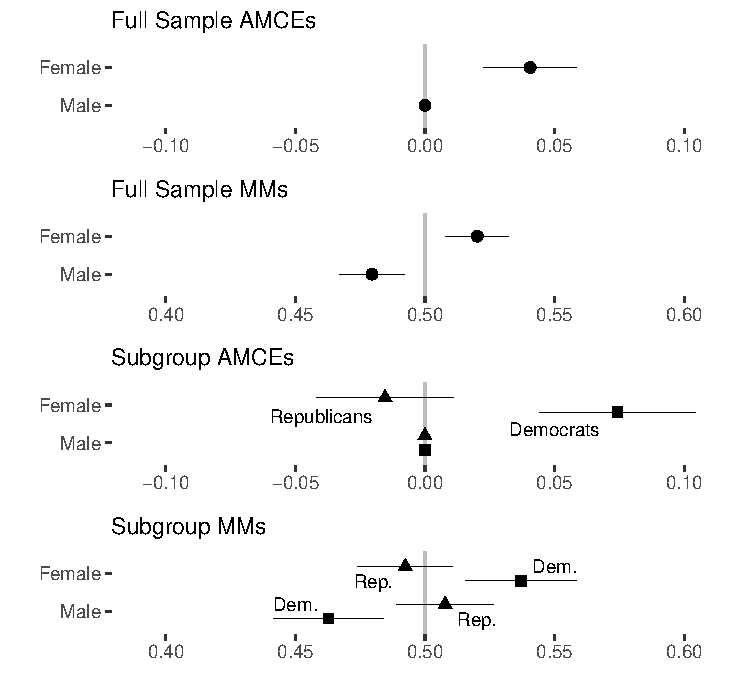
\includegraphics[width=\maxwidth]{figure/tkr_replication-1} \caption[Replication of Results for `Candidate Sex' Feature from Teele et al]{Replication of Results for `Candidate Sex' Feature from Teele et al. (2018) Candidate Experiment using Full Sample and Subgroup AMCEs and MMs}\label{fig:tkr_replication}
\end{figure}


\end{knitrout}

Yet, just as analysis of full sample conjoint data is often descriptive in nature, so too do conjoint analysts frequently interpret differences in conditional AMCEs descriptively rather than causally. For example, in one analysis \citet{HainmuellerHopkinsYamamoto2014} visually compare the pattern of AMCEs among high- and low-ethnocentrism respondents and interpret that ``the patterns of support are generally similar for respondents irrespective of their level of ethnocentrism'' (22). \citet{BallardRosaMartinScheve2016} make similar comparisons in their tax policy conjoint: ``While there are few strong differences in preferences for taxing the lower three income groups (the `hard work' group has slightly lower elasticities for taxing the poor), there are strong differences in preferences for taxing the rich'' (12). In \citet{BechtelScheve2013} conjoint on support for international climate change agreements in the United States, United Kingdom, Germany, and France, they summarize their results as ``We find that individuals in all four countries largely agree on which dimensions are important and to what extent'' (13765). In these examples, the differences between conditional AMCEs are used as a way of descriptively characterizing differences in \textit{preferences} (i.e. levels of support) between the groups rather than differences in \textit{causal effects on preferences} in the groups.

The selection of a reference category, while earlier an innocuous analytic decisions, becomes substantially consequential for this kind descriptive reading of conditional AMCEs. Most obviously, using AMCEs descriptively prevents analysts from describing levels of favorability in the reference category but also can lead to misinterpretations of patterns in preferences. AMCEs are relative, not absolute, statements about preferences. As such, there is simply no predictable connection between subgroup causal effects and the levels of underlying subgroup preferences. Yet analysts and their readers frequently interpret differences in conditional AMCEs as differences in underlying preferences. While AMCEs do provide insight into the descriptive variation in preferences within-group and across-features, and conditional AMCEs do estimate the size of causal effects of features within groups, AMCEs cannot provide direct insight into the pattern of preferences between groups because they do not provide information about \textit{absolute} levels of favorability toward profiles with each feature (or combination of features).

This additional information matters. Consider again the simple two-condition experiment in which the effect of a male as opposed to female candidate, $x \in {0,1}$, is compared across a single two-category covariate, $z \in {0,1}$ such as Democratic or Republican self-identification. Subgroup regression equations to estimate effects for each group are:

\begin{align*}
\hat{y} &= \beta_0 + \beta_1 x + \epsilon, \quad \forall z = 0 \\
\hat{y} &= \beta_2 + \beta_3 x + \epsilon, \quad \forall z = 1
\end{align*}

\noindent The effect of $x$ when $z=0$ is given by $\beta_1$. The effect of $x$ when $z=1$ is given by $\beta_3$. These are, in essence, the conditional AMCEs in a conjoint analysis. Yet the difference in AMCEs ($\beta_3 - \beta_1$) is not equal to the difference in preferences between the two groups, which is $\bar{y}_{z=1|x=1} - \bar{y}_{z=0|x=1}$ (estimated by $(\beta_2 + \beta_3) - (\beta_0 + \beta_1)$). The difference-in-AMCEs only equals the difference in preferences when $\beta_2 \equiv \beta_0$. Yet the standard AMCE-centric conjoint analysis does not present or characterize absolute favorability in the reference category. Similarity of conditional AMCEs only means similarity of the \textit{causal effect} of the feature across groups, not similarity of \textit{preferences} unless preferences toward profiles with the reference category are equivalent in both groups. Given the reference category choice is typically arbitrary or driven by substantive knowledge of the levels, there is never any reason to expect that an arbitrarily selected reference category satisfies this equality requirement. When using a difference-in-AMCEs comparison to estimate a difference in preferences, the size and direction of the bias is determined by the size of the difference in preferences toward the reference category within each subgroup.

To draw this example out more fully, the upper panel of Figure \ref{fig:tkr_replication} shows AMCEs for \citeauthor{TeeleKallaRosenbluth2018}'s candidate choice experiment for the full sample of respondents. The second panel shows full sample marginal means. The third panel shows conditional AMCEs separately for Democratic and Republican voters, as provided in the original paper and the lower panel shows the results using conditional marginal means for Democratic and Republican voters.\footnote{We opt here for visual presentation of results; tabular presentation of AMCEs, marginal means, and associated standard errors for all examples are included in the Appendix.} Respondents' preference for female candidates is very apparent in both forms of analysis in the upper two panels because the AMCE definitionally equals the difference in marginal means. But how do Republicans and Democrats differ in their preferences over male and female candidates? By requiring a reference category fixed to zero, the conditional AMCE results in the third panel suggest that there is a very large difference in favorability toward female candidates between Republican and Democratic respondents. In reality, however, the difference in these conditional AMCEs (0.086) reflects the true difference in favorability toward female candidates (difference: 0.045; Democrats: 0.537, Republicans: 0.492) \textit{plus} the difference in favorability toward male candidates (difference: 0.045; Democrats: 0.463, Republicans: 0.508). Because Democrats and Republicans actually differ in their views of profiles containing the reference (male) category, AMCEs sum the true differences in preferences for a given feature level with the difference in preferences toward the reference category.\footnote{Another example that clearly demonstrates the discrepancy between the differences in preferences and the differences in conditional AMCEs can be seen very clearly in the ``political experience'' feature of this experiment (see Supporting Materials). The conditional AMCEs correctly convey that both Democrats and Republicans are more likely to favor experienced than inexperienced candidates. Reading the AMCEs descriptively, however, would suggest that Democratic voters are more favorable toward candidates with all levels of experience compared to Republican voters (i.e., Republicans and Democrats differ in their preferences over experienced candidates). In reality, however, the conditional marginal means reveal that actually Democrats and Republicans have very similar preferences toward candidates with 1 or 3 years of experience, but differ dramatically in their preferences over candidates with no experience (the reference category) and those with 8 years experience. Democrats are much more sensitive to experience than are Republicans and important differences in preferences between the groups are apparent for very high and very low experience, but the conditional AMCEs suggest that preferences differ at all levels of experience, when in reality they do not.}


\begin{knitrout}
\definecolor{shadecolor}{rgb}{0.969, 0.969, 0.969}\color{fgcolor}\begin{figure}
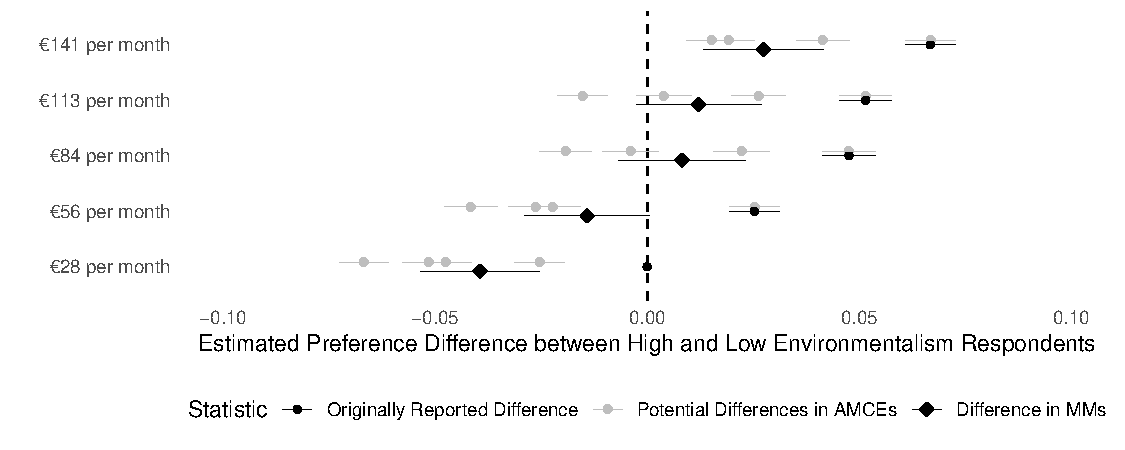
\includegraphics[width=\maxwidth]{figure/bechtel_difference_comparison-1} \caption[True Difference in Favorability and Implied Preference Differences between High and Low Environmentalism Respondents for `Monthly Cost' Feature from Bechtel and Scheve (2013) Climate Agreement Experiment for Each Possible Reference Category]{True Difference in Favorability and Implied Preference Differences between High and Low Environmentalism Respondents for `Monthly Cost' Feature from Bechtel and Scheve (2013) Climate Agreement Experiment for Each Possible Reference Category}\label{fig:bechtel_difference_comparison}
\end{figure}


\end{knitrout}



We can also see this bias clearly in a reanalysis of \citeauthor{BechtelScheve2013}'s four-country climate change agreement experiment. Figure \ref{fig:bechtel_difference_comparison} shows an analysis for the feature capturing the monthly household cost for a potential international climate agreement, replicating a portion of the results they present comparing high- and low-environmentalism respondents (pooling across countries) \citet[13767 figure 4]{BechtelScheve2013}. The original analysis was presented as conditional AMCEs for the two subgroups with 28 Euro per month as the reference category. Conditional AMCEs for both groups were presented as negative with conditional AMCEs for low-environmentalism respondents being more negative than the conditional AMCEs for high-environmentalism respondents at every feaure level. This implies positive differences in favorability toward each monthly cost between high- and low-environmentalism respondents. Figure \ref{fig:bechtel_difference_comparison} presents the implied difference-in-AMCEs from the original analysis as black circles, demonstrating the substantial and positive \textit{apparent} differences between the two groups. For example, the difference-in-AMCEs for the 56 Euro per month level (incorrectly) implies that high-environmentalism respondents are \textit{more} favorable toward a 56 Euro per month household cost of an agreement than are low-environmentalism respondents. Yet the opposite is actually true: high environmentalism respondents are less favorable toward this option than low environmentalism respondents. By using the 28 Euro per month level as the reference category, the original analysis implies that preferences are identical between the two groups when in reality high-environmentalism respondents are much less favorable toward a 28 Euro per month cost than low-environmentalism respondents. The black diamonds in Figure \ref{fig:bechtel_difference_comparison} show these true differences in favorability as marginal means for the two groups.

Furthermore, the gray dots in Figure \ref{fig:bechtel_difference_comparison} represent the alternative differences-in-AMCEs that \textit{could have been generated} from alternative choices of reference category using the same data. Not only is it possible for reference categories choice to significantly color the apparent size of differences between subgroup, that choice can also impact the direction and statistical significance of subgroup differences. An analyst could easily choose a reference category that presents differences between these two group as large and positive, small and positive, small and negative, large and negative, or negligible. The original analysis (again, black circles) happens to show large and positive differences between the groups.

It is worth highlighting two further features in Figure \ref{fig:bechtel_difference_comparison}. First, the alternative differences-in-AMCEs estimates vary mechanically around the difference in marginal means, as the reference category varies (just as the AMCE estimates did in Figure \ref{fig:reference_category}). The difference between marginal means for two groups are always fixed in the data, so the differencing of subgroup AMCEs is merely an exercise is centering those differences at arbitrary points along the range of observed differences in marginal means. Differences-in-AMCEs for a given feature level must therefore necessarily sometimes be positive and sometimes be negative, depending on the reference category used in estimating them. The direction of the difference per se conveys no information about underlying pattern of preferences in the two groups. 

Second, and more practically, because there is no category for which the preferences of the two subgroups in this example are identical, no choice of reference category would have led to inferences from differences-in-AMCEs that accurately reflect the underlying difference in preferences. Even in the 84 Euro per month level, the difference between the two groups is slightly positive. Were there a category for which subgroup preferences were exactly equal, that could be sensibly chosen as the reference category in order to be able to interpret differences-in-AMCEs as differences in preferences. But there is never any guarantee, however, that such a reference category exists in any given experimental dataset. If multiple subgroup analyses are performed, it is unlikely the same reference category would work well across all analyses, making consistent interpretation difficult. And because conjoint analysis generates a sparse feature matrix (where there is never any guarantee that a particular combination of feature levels is observed in the data), it is also not possible to empirically select an appropriate set of reference categories using the observed data. It is impossible to know which cell --- of the tens of thousands in the design --- is the best choice of reference. Indeed it is possible that there is no such cell for which preferences are identical in the two groups; such a cell may exist, but there is no reason to expect that it should exist in any given application or that it would happen to be observed. Thus, there is no way to use conditional AMCEs or differences between those conditional AMCEs to convey the underlying similarity or differences in preferences across sample subgroups.


\section*{Improved Analysis of Subgroup Preferences in Conjoint Designs}\label{sec:marginalmeans}



\begin{knitrout}
\definecolor{shadecolor}{rgb}{0.969, 0.969, 0.969}\color{fgcolor}\begin{figure}
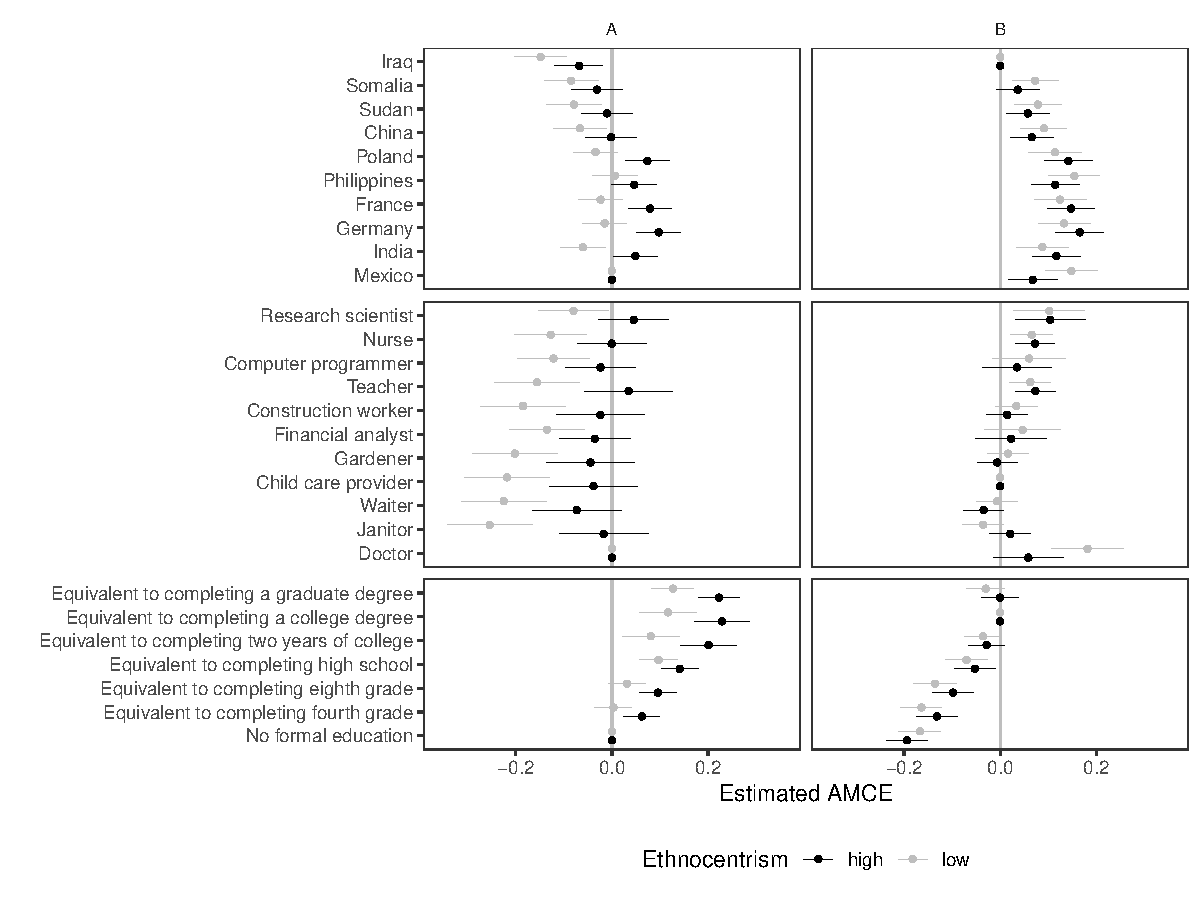
\includegraphics[width=\maxwidth]{figure/hainmueller_subgroup_example_plot-1} \caption[Comparison of AMCEs for Low- and High-Ethnocentrism Respondents Using Two Alternative Reference Categories Choices for Hainmueller et al]{Comparison of AMCEs for Low- and High-Ethnocentrism Respondents Using Two Alternative Reference Categories Choices for Hainmueller et al. (2014) Immigration Experiment}\label{fig:hainmueller_subgroup_example_plot}
\end{figure}


\end{knitrout}

We have shown that subgroup analyses of conjoint designs frequently entail the use of difference-in-AMCE comparisons and we have also shown that such analyses, perhaps counterintuitively, do not demonstrate differences in preferences between groups due the near-impossibility of selecting a non-arbitrary reference category against which to estimate AMCEs. Thus the choice of reference category --- while seemingly irrelevant --- has dramatic inferential consequences in conjoint analyses. Here we provide a more complete example, demonstrating the full extent of this problem for interpretation of conjoint results and present alternative forms of analysis that more robustly convey subgroup preferences and the differences (if any) between them. Specifically, we show how reference category changes can lead to visual patterns of differences-in-AMCEs that provide strikingly different interpretations. We then show how to visualize and formally compare subgroup marginal means using simple means comparisons tests to avoid this problem. Finally, we demonstrate how to use nested model comparison tests to formally test for omnibus differences between groups.

Consider the left and right facets of Figure \ref{fig:hainmueller_subgroup_example_plot}, which show the exact same analysis (comparing AMCEs for high and low ethnocentrism respondents) on the same experimental data from \citeauthor{HainmuellerHopkinsYamamoto2014}'s immigration experiment. In panel ``A'' (left), all features are configured so that the reference category is the one with the largest difference in preferences between the two subgroups. In panel ``B'' (right), all features are configured so that the reference category is the one with the smallest difference in preferences between the two subgroups.\footnote{The appendix contains comparable plots for experiments by \citet{BallardRosaMartinScheve2016} and \citet{TeeleKallaRosenbluth2018}.}

Panel A gives the impression that there are significant differences in preferences between high and low ethnocentrism respondents toward immigrants from different countries of origin, with different careers, and with different educational attainments. By contrast, Panel B gives the impression that these differences --- indeed all differences --- are negligible. The experimental data and analytic approach in the two portrayals is identical; the only difference is the choice of reference category for the profile features. Given what we have shown about the relationship between differences in conditional AMCEs and differences in conditional marginal means, Panel B is the more truthful visualization \citep{Cairo2016}. The differences between subgroup AMCEs there more accurately convey differences in underlying preferences because the reference categories used in Panel B are the most similar between the two groups. Yet even this may not \textit{perfectly} convey differences because no feature generates perfect agreement between the subgroups.

\begin{knitrout}
\definecolor{shadecolor}{rgb}{0.969, 0.969, 0.969}\color{fgcolor}\begin{figure}
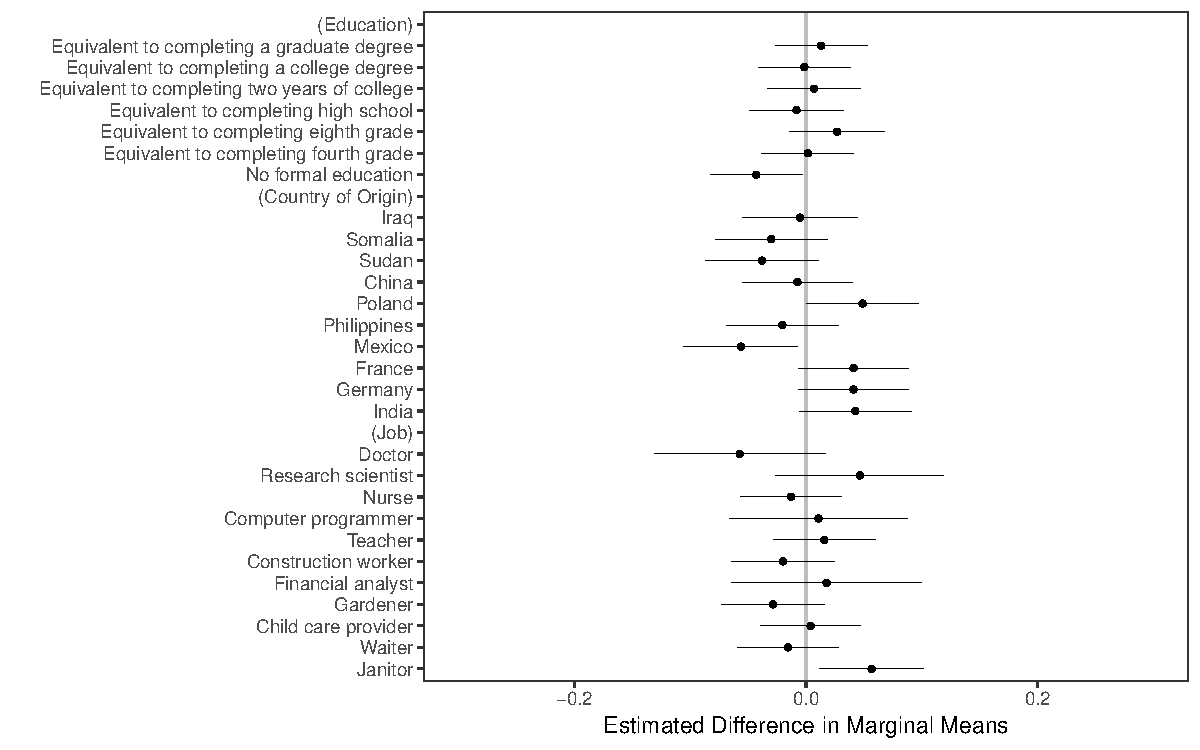
\includegraphics[width=\maxwidth]{figure/hainmueller_mm_diffs-1} \caption[Differences in Conditional Marginal Means, by Ethnocentrism, for Hainmueller et al.'s (2014) Immigration Experiment]{Differences in Conditional Marginal Means, by Ethnocentrism, for Hainmueller et al.'s (2014) Immigration Experiment}\label{fig:hainmueller_mm_diffs}
\end{figure}


\end{knitrout}

Alternatively presenting subgroup differences using conditional marginal means (as in Figure \ref{fig:hainmueller_mm_diffs}) provides the intended descriptive comparison of subgroup preferences. Each dot and error bar represents the conditional marginal mean (and its standard error) for high ethnocentrism (in red) and low ethnocentrism (in blue) respondents. This display of conditional marginal means highlights just how similar the preferences are for the two groups. For example, in the first set of estimates, both groups of respondents display minimally positive preferences toward female immigrants and minimally negative preferences toward male immigrants, averaging across those immigrants' other profile features. The second set of estimates shows both group are also more favorable toward higher-educated immigrants and less favorable toward less-education immigrants with no visually apparent differences. The third set of estimates, related to language skills, shows again similar patterns: both groups are more favorable toward immigrants with higher English proficiency than immigrants with lower English proficiency.

These estimates are less obviously identical for the two groups but look quite close. To test for pairwise differences between high and low ethnocentrism respondents, we can calculate differences in conditional conditional marginal means at each feature level, with associated significance tests:

\begin{itemize}
\item spoke fluent English: 0.02 (0.02, $z_{\text{diff}}$=1.30, $p\leq 0.20$)
\item spoke broken English: 0.01 (0.02, $z_{\text{diff}}$=0.71, $p\leq 0.48$)
\item tried to speak English but was unable: -0.01 (0.02, $z_{\text{diff}}$=-0.78, $p\leq 0.43$)
\item spoke [language] and used an interpreter: -0.02 (0.02, $z_{\text{diff}}$=-1.22, $p\leq 0.22$)

\end{itemize}



\noindent These pairwise tests show that are our eyes have not deceived us. None of the level-specific differences in conditional marginal means are statistically distinguishable from zero. Were we interested in an omnibus tests of whether any of these differences were non-zero, we could perform a nested model comparison of two equations: (a) one estimating only marginal effects of the ``Language Skills'' feature levels, and (b) the same model with additional interactions between the subgrouping covariate and the feature levels. The test compares the sum of squared residuals for the two equations.

To make this concrete, for a feature with four levels (one treated as a reference category), the first (restricted) equation would be:

\begin{equation}\label{eq:restricted}
Y = \beta_0 + \beta_1 Level_1 + \beta_2 Level_2 + \beta_3 Level_3 + u
\end{equation}

\noindent The second (unrestricted) equation would allow for interactions between feature levels and the subgroup identifier:

\begin{equation}\label{eq:unrestricted}
\begin{split}
Y = & \beta_0 + \beta_1 Level_1 + \beta_2 Level_2 + \beta_3 Level_3 + \beta_4 Group + \\
& \beta_5 Level_1 * Group + \beta_6 Level_2 * Group + \beta_7 Level_3 * Group + u
\end{split}
\end{equation}

\noindent While Equation \ref{eq:restricted} imposes the constraint that $\beta_4 = \beta_5 = \beta_6 = \beta_7 = 0$, Equation \ref{eq:unrestricted} allows for subgroup differences in favorability. The nested model comparison allows us to test the joint null hypothesis that there are no differences between the subgroups in any of the feature levels. This entails computing an F-statistic:

\begin{equation}
F = \dfrac{\dfrac{SSR_{Restricted} - SSR_{Unrestricted}}{r}}{\dfrac{SSR_{Unrestricted}}{n - k - 1}}
\end{equation}

\noindent where $SSR_{Restricted}$ is the sum of squared residuals for Equation \ref{eq:restricted}, $SSR_{Unrestricted}$ is the sum of squared residuals for Equation \ref{eq:unrestricted}, where $r$ is the number of restrictions (in the above example, 4), $n$ is the number of cases, and $k$ is the number of feature levels in the unrestricted model. Note that this test is not sensitive to reference category used in the regression 


For the \citeauthor{HainmuellerHopkinsYamamoto2014} language feature, the resulting F-test for the model comparison in this case again gives us little reason to believe there are subgroup differences: F(4, 11496)=1.06, $p\leq0.37$. We could repeat such pairwise comparisons or omnibus comparisons for each feature in the design.

Furthermore, we could also directly visualize differences in conditional marginal means for this feature --- and all features --- as in Figure \ref{fig:hainmueller_mm_diffs}. This provides a more direct presentation of \textit{differences} between subgroup preferences as the vertical line indicates feature levels for which there is no difference between the two groups. Positive values to the right of the line indicate positive differences (high ethnocentrism respondents are more favorable toward immigrants with this feature than low ethnocentrism respondents) and negative value to the left of zero convey the opposite. A further advantage of this plot is that unlike displays of conditional AMCEs, differences in conditional marginal means communicate subgroup differences for all feature levels including the reference categories. This display makes readily clear what was only indirectly apparent in Figure \ref{fig:hainmueller_mm_diffs}: there are indeed no sizeable and only a few statistically apparent differences in preferences between the two groups.





As before, we can perform an omnibus tests for the presence of any subgroup differences across all features, again using nested model comparison of two equations: (a) one estimating only effects of the features, and (b) the same model with additional interactions between the subgrouping covariate and all features. The result of that test for differences by ethnocentrism from the immigration experiment is: F(98, 11402)=1.16, $p\leq0.14$, which further demonstrates that the substantive interpretation provided by \citet{HainmuellerHopkinsYamamoto2014} accurately identified a lack of between-group differences. By contrast, \citet{BechtelScheve2013} argue in their cross-country conjoint examining climate change agreements ``that individuals in all four countries largely agree on which dimensions are important and to what extent'' \citep[13765]{BechtelScheve2013}. Yet a nested model comparisons shows the countries do differ in their preferences F(54, 67982)=3.72, $p\leq0.00$. This cross-country variation is largely driven by differences in sensitivity to monthly household costs feature, F(15, 67995)=3.80, $p\leq0.00$, with the United Kingdom and United States being more cost sensitive than Germany and France as is plainly visible in a plot of marginal means by country (see SI).

This kind of nested model comparison test can also be used to assess heterogeneity across conjoint features \citep[see also][]{EgamiImai2018}. For example, \citet{TeeleKallaRosenbluth2018} report just such a test for how effects of features other than candidate sex may differ between male and female candidates, finding no such heterogeneity (8--9). Fortunately, the original analysis accurately detected an absence of subgroup differences, yet a subtly different set of analytic decisions about reference categories (as shown in Figure \ref{fig:hainmueller_subgroup_example_plot}) could have led to an quite different conclusion.

\section*{Conclusion}\label{sec:conclusion}

This article has identified several challenges related to the analysis and reporting of conjoint experimental designs, particularly analyses of subgroup differences. We suggest that conjoint analyses should report not only average marginal component effects (AMCEs) but also descriptive quantities that better convey underlying preferences over profile features and better convey subgroup differences in those preferences. Our intention here is not to substantively undermine any previous set of results but instead to urge researchers moving forward to demonstrate considerable caution in how they design, analyze, and present the results of these types of descriptive experiments. We have relatively straightforward and hopefully uncontroversial advice for how analysts of conjoint experiments should proceed:

\begin{enumerate}
\item Always report unadjusted marginal means when attempting to provide a \textit{descriptive} summary of respondent preferences in addition to or instead of AMCEs.\footnote{Like the presentation of AMCEs, displaying marginal means in constrained conjoint designs may also distort apparent patterns given that not all features can co-occur. Partitioning the design into fractions such that each fraction contains a fully unconstrained design would mitigate any concern with that presentation.}

\item Exercise caution when explicitly or implicitly interpreting differences-in-AMCEs across subgroups. Differences-in-AMCEs are differences in effect sizes for subgroups, not statments about the relative favorability of the subgroups toward profiles with a feature. Heterogeneous effects do not necessarily mean different underlying preferences. If differences in AMCEs are reported, the choice of reference categories should be discussed explicitly and diagnostics should be provided to justify it.

\item When descriptively characterizing differences in preferences between subgroups, directly estimate the subgroup difference using conditional marginal means and differences between conditional marginal means, rather than relying on the difference-in-AMCEs.

\item To formally test for group differences in preferences, regression with interaction terms between the subgrouping covariate and all feature levels will generate estimates of level-specific differences in preferences via the coefficients on the interaction terms.\footnote{The analysis is slightly more complicated in constrained designs.} A nested model comparison between this equation against one without such interactions provides an omnibus test of subgroup differences, which should be reported when characterizing overall patterns of subgroup differences.
\end{enumerate}

\noindent Following this advice, we hope, will allow researchers to more clearly and more accurately represent descriptive results of conjoint experiments.

The popularity of conjoint analyses in recent years highlights the power of the design and the important contributions made by \citet{HainmuellerHopkinsYamamoto2014} in providing a novel causal interpretation of these fully randomized factorial designs. Yet with new tools always come new challenges. The now-common practice of descriptively interpreting conjoints requires more caution than is immediately obvious. This paper has demonstrated several such challenges and hopefully provides useful advice for how researchers should proceed with the analysis of such designs.

To facilitate such analysis and, especially, to provide easy-to-use tools for calculating marginal means and performing reference category selection diagnostics, we provide software called \textbf{cregg} \citep{Leeper2018cregg} that will perform these analyses and also provides the simple-to-use visualization tools used throughout this article. With that resource in-hand, researchers should be well-equipped to analyze conjoint designs without running into the analytic challenges discussed here.



\singlespacing
\bibliographystyle{apsa-leeper}
\bibliography{references}
\clearpage


\appendix
\tableofcontents



\clearpage

\section{Definition of Quantities of Interest}\label{app:quantities}

A conjoint experiment serves two purposes: (1) description of the conditional distribution of favorability over variations in multiple features, and (2) leveraging the random observation of combinations of features (so-called ``profiles'') to infer that any differences in favorability over features are causally attributable to the features as opposed to something else. The quantities of interest are therefore functions of the features being randomized as in any factorial experiment. But additionally, conjoints typically involve within-subjects research designs (i.e., multiple, different profile observations per participant) thus necessitating some additional notation to account for the \textit{survey implementation} of the conjoint in addition to the definition of the descriptive and causal parameters of interest.

Ultimately, a conjoint since \citet{HainmuellerHopkinsYamamoto2014} is a complex survey-experimental design involving multiple observations across a high-dimension factorial experimental space. Specifically, $I$ respondents ($i \in \{1, \dots, I\}$) are presented with $K$ rating or forced choice decision tasks, each involving $J$ (typically 2) alternative profiles of, for example, candidates or policies. Each profile consists of a vector of $F$ (typically discrete) features or attributes that describe the profile (e.g., age, sex), each composed of $D_f$ alternative levels, a number which can vary across features. The experiment thus generates a dataset with $N = I \times J \times K$ observations of some rating scale or discrete choice outcome, $Y$, from a random sample of profiles drawn from the $C = \prod_{f = 1}^{F} D_f$ population of experimental \textit{cells} in the $F$-dimension feature space.

The survey implementation of the conjoint therefore generates $N$ observations that can be indexed by $i,j,k$, forming an $N \times(L+4)$ dimensional data matrix $\mathbf{M}$ with each row representing the vector of feature levels $\vec{F}$ in each profile $j$ of respondent $i$'s task $k$, with indicators for $i$, $j$, $k$, and the corresponding outcome $Y_{i,j,k}$.\footnote{In typical paired designs (where $J=2$), this means each task generates two data points: $Y_{i,1,k}$ and $Y_{i,2,k}$. Note, too, that in fully randomized designs, these two profiles can be identical. Furthermore in fully randomized, forced-choice designs this can yield the additional curiosity that $Y_{i,\mathbf{c}} \neq Y_{i,\mathbf{c}}$ for a given respondent, $i$, and profile, $\mathbf{c}$.}

With no loss of information, we can think of each row in this matrix equivalently as an observation of $Y_{i,\vec{F}}$. This is because \citet{HainmuellerHopkinsYamamoto2014} make several important assumptions that allow us to interpret these data in a different way than the survey implementation implies. First, they assume no carryover effects (Assumption 1), such that multiple observations from the same respondent can be treated as independent of one another. Second, they assume no profile order effects within-task (Assumption 2), such that profiles within a task can be treated as independent of each other. Assumptions 1 and 2 imply that the survey implementation indices for task, $k$, and profile-within-task, $j$, can be ignored. They have no bearing on any quantity of interest, by assumption. 

The analyst is therefore left with a dataset of $N$ observations, grouped into $i$ participants, each providing into $Y_{\vec{F}}$. All quantities of interest must therefore be specified over as features of the distribution of $Y$ over the $F$-dimensional feature space. In what follows, we therefore focus on the experimental features being randomized rather than the survey design factors being assumed away. \citet{HainmuellerHopkinsYamamoto2014} make a third assumption that profiles are randomly constituted (Assumption 3), which in a fully randomized design, has the effect of meaning that features and feature combinations are randomly sampled for observation. If this randomization is uniform (which it almost always is in applied examples) this means we can additionally ignore the probability of observing any given combination (as all profiles are equally likely to be observed). This is a point we return to in a moment.

The most basic thing that can be estimated about the distribution of $Y$ is the expected value, $E[Y]$, or \textit{grand mean} (in the parlance of factorial experiments). We can think of this quantity in terms of the survey implementation process (namely, respondents, tasks, and profiles) or as a simple function of the resulting data:

\begin{equation}
\bar{Y} = \dfrac{1}{I \times J \times K} \sum_{i=1}^{I} \sum_{j=1}^{J} \sum_{k=1}^{K} Y_{i,j,k} = \dfrac{1}{N} \sum_{n=1}^{N} Y_n
\end{equation}

\noindent The nested summation over $i,j,k$ could be stated explicitly but is unnecessary as the grand mean is simply the mean of all observed $Y$. A useful check on intuition is that in a forced choice design, where a respondent must choose only one profile, $j$, of all those presented in each task $k$, then by design $\bar{Y} = \frac{1}{J}$. For common, two-alternative, forced choice designs, $\bar{Y}$ therefore always equals $0.5$. By contrast, in rating scale designs, $\bar{Y}$ can take any value between the lower and upper bounds of the rating scale.

In a \textit{full factorial} experiment where $N > C$ (the number of observations is larger than the number of cells) due to a large sample, or few factors, or levels of each factor, or both (or both of these design characteristics), a sensible next quantity of interest is the \textit{cell mean}: $E[Y|\vec{X} = \vec{x}]$, which in a conjoint simply measures the mean favorability toward a particular profile, $\vec{x}$. An effort to actually estimate this quantity will, however, become obviously intractable when one recognizes that the number of observations in a typical conjoint is much lower the number of feasible profiles ($N \ll C$). The cell mean can be unobserved for many or perhaps most experimental cells. 

Therefore quantities of interest that derive from it --- such as pairwise differences of means between cells --- cannot be estimated for any of the arbitrary $\binom{C}{2}$ pairs of cells. As an example, in the \cite{HainmuellerHopkinsYamamoto2014} candidate experiment, $C = 6^6 * 2^2 = 186,624$ and $N = 3466$, so less than 2\% of experimental cells were observable and a minuscule fraction of the 17.4 billion pairwise cell combinations could have generated estimable effects. 

It is at this point that the quantities of interest in a conjoint can become confusing. In a typical experiment where $N > C$, these pairwise differences of means are the standard estimator for a causal effect (the estimand being the causal effect on favorability of changing from one profile to another). For example, we might be interested in the effect on $Y$ of changing the value of one feature to another theoretically interesting value of that feature, holding all other feature values in the profile constant:

\begin{equation}
\tau = E[Y|X_1=x_1,X_2=x_2,\dots,X_f=x_f] - E[Y|X_1= \neg x_1,X_2=x_2,\dots,X_f=x_f]
\end{equation}

\noindent but we have no guarantee that both or, in fact, either of those particular cells are observed. If even this minimal causal quantity cannot be guaranteed to be estimable by design, questions about higher-order interactions across features are even more difficult to estimate as they require observing four or more specific cells, any of which may be missing. Even if we were interested in such quantities, we would be unlikely to be able to estimate them.

Conjoint designs therefore ask us to think about completely different quantities of interest from typical sentiment measurement or experimentation. Consequently, what quantities might we care about that can be estimated from an $L$-dimension factorial experimental with considerable sparsity other than the grand mean? 

Even though $N \ll C$ in most applied conjoints, $N > F$. This means that even if we probably cannot learn about particular high-dimensional \textit{combinations of features}, we can learn about favorability toward particular features alone. That is, we can learn about conditional expectations over each feature dimension, $E[Y|X_f=x_f]$. In the factorial experiments literature, this conditional mean is called the \textit{marginal mean} (as it lies at the margins of a tabular presentation cell means for the complete design). For example, the following 2x3 factorial design contains 6 cell means ($2*3$), 1 grand mean, and five marginal means ($2+3$, one for each level of each factor):

\begin{center}
\begin{tabular}{lccc}\toprule
 & $A = 1$ & $A = 2$ & \\ \midrule
$B = 1$ & $\bar{Y}_{A=1, B=1}$ & $\bar{Y}_{A=2, B=1}$ & $E[Y|B=1]$ \\
$B = 2$ & $\bar{Y}_{A=1, B=2}$ & $\bar{Y}_{A=2, B=2}$ & $E[Y|B=2]$ \\
$B = 3$ & $\bar{Y}_{A=1, B=3}$ & $\bar{Y}_{A=2, B=3}$ & $E[Y|B=3]$ \\ \midrule
 & $E[Y|A=1]$ & $E[Y|A=2]$ & $E[Y]$ \\ \bottomrule
\end{tabular}
\end{center}

The uniform sampling of cells in the design means that this is quantity can be estimated by the simple mean of $Y \forall X_f = x_f$.\footnote{In unbalanced designs where the probability of being in a given cell is not uniform across cells, there is sometimes a distinction made between \textit{descriptive} marginal means that equally weight observations and \textit{design} marginal means that equally weight cells in the design. Given conjoint designs generally do not allow for the observation of cell means, the distinction is not relevant and we refer to \textit{descriptive} marginal means simply as ``marginal means.''}

Were a constrained conjoint design used where some feature combinations were impossible, the marginal means would only be intelligible in the fractions of the design where all cells are observed.\footnote{Practically, the random sampling of cells does not need to be uniform; over- and under-representation of cells is possible. We focus here on fully randomized designs that draw profiles from the full space with equal probability. A nuance in \citeauthor{HainmuellerHopkinsYamamoto2014}'s notation is that their quantities of interest are conditioned on an arbitrary joint distribution of features rather than the particular joint distribution of features that was used to construct design or the joint distribution of features that happens to emerge empirically. In other words, they weight cells by an arbitrary joint probability mass function.}

To clarify this point, consider the constrained 2x3 design below where one cell is unobserved by design:

\begin{center}
\begin{tabular}{lccc}\toprule
 & $A = 1$ & $A = 2$ & \\ \midrule
$B = 1$ & $\bar{Y}_{A=1, B=1}$ & $\bar{Y}_{A=2, B=1}$ & $E[Y|B=1]$ \\
$B = 2$ & $\bar{Y}_{A=1, B=2}$ & $\bar{Y}_{A=2, B=2}$ & $E[Y|B=2]$ \\
$B = 3$ & $\bar{Y}_{A=1, B=3}$ & -- & $E[Y|B=3]$ \\ \midrule
 & $E[Y|A=1]$ & $E[Y|A=2]$ & $E[Y]$ \\ \bottomrule
\end{tabular}
\end{center}

\noindent Were the lower-right cell ($A=2, B=3$) observable by design, then a direct comparison of the marginal means, $E[Y|A=1]$ and $E[Y|A=2]$, in the lower table margin would provide direct insight into the relative favorability of respondents to profiles with features $A=1$ and $A=2$, marginalized over $B$. But because this cell is unobserved, these marginal means marginalize over different subsets of the possible values of $B$ making them not obviously comparable. By contrast, the first and second marginal means at the top-right of the table --- $E[Y|B=1]$ and $E[Y|B=2]$ --- provide insight into the favorability of participants toward profiles with features $B=1$ and with feature $B=2$ marginalizing over the two possible values of $A$. A researcher could safely conclude that participants are more (less) favorable toward profiles with feature $B=1$ than $B=2$ from this information alone. But they would not be able to so for feature $A$ without either (a) an explicit caveat that the comparison is of dissimilar subsets of profiles along dimension $B$ or (b) calculating marginal means over only the completely observable\footnote{Note that what matters here is \textit{observability}, not whether any given cell is actually observed. We know from above that most cells will be unobserved even in a uniformly sampled, unconstrained design.} portion of the feature space due to the curse of dimensionality.

For the common \textit{descriptive} use of conjoint designs to measure preferences over multi-dimensional objects, these marginal means alone are of direct interest. They express favorability on the scale of the outcome over alternative values of each feature independent of the features in the design.\footnote{They do not necessarily convey favorability in an absolute sense. A high marginal mean for a given feature does not imply that the sample prefers that feature in an absolute sense. Instead, favorability has to be understood in light of the features presented to respondents. This is the innovation in conjoints; rather than asking respondents whether they will support a Mormon candidate (for example), we can infer their favorability toward a Mormon candidate in light of other candidate characteristics they may consider. Still our design may not contain all such features, so caution is needed in drawing typical public opinion inferences from these marginal means.}

For the \textit{causal} interpretation of conjoint designs, comparisons of these marginal means is required. Comparisons between them provide causal inferences about the effect of changing a focal feature, marginalizing across the distribution of other features. Because feature combinations (i.e., the profiles) are randomly constructed and randomly observed from all possible combinations, the distribution of other non-focal features is, in expectation, is independent of the focal feature, thus identical across all levels of the focal feature, and therefore ignorable.

A typical causal effect of interest is therefore the difference in marginal means across two levels of a feature (i.e., the marginal effect of a change in a feature's levels). For an unconstrained design, this difference is the \textit{average marginal component effect} (AMCE) defined by \citet{HainmuellerHopkinsYamamoto2014}. In this way, an AMCE is simply a marginal effect of the factorial design: the difference of two marginal means.

Unfortunately, this is not a perfectly complete definition, but it covers the vast majority of applied cases. The exceptions are few. First, \citeauthor{HainmuellerHopkinsYamamoto2014} allow the joint distribution of features used in calculating the difference of marginal means to be arbitrary. This is meant to accommodate the weighting of marginal means to reflect the real-world distribution of feature combinations (e.g., down-weighting African American Republican political candidates given their rarity in real-world politics). Their definition of an AMCE allows for arbitrary weighting, but in practice this is uncommon.

Second, in constrained designs where some cells are unobservable, care needs to be taken in both defining and estimating AMCEs. Take, for example, the trivial example just above. The difference $E[Y|B=2]-E[Y|B=1]$ marginalizes over the full set of levels of $A$ but $E[Y|B=3]-E[Y|B=1]$ marginalizes only over case where $A=1$. Thus these two marginal effects reflect different subsets of the data and different combinations of values of $A$.

\citeauthor{HainmuellerHopkinsYamamoto2014} allow for these two differences to be presented as the AMCE despite the fact that the quantities marginalize over distinct subsets of the design. Indeed, their definition of AMCE for constrained designs diverges from the intuitive marginal effect to instead define the AMCEs for levels of $B$ as an average of marginal effects of $B$ over subsets of $A$ and the AMCEs for levels of $A$ as averages of the marginal effects of $A$ over subsets of $B$ (again, weighting these marginal effects arbitrarily). For example, if feature $A$ is race ${Caucasian, African American}$ and feature $B$ is religion ${Evangelical, Catholic, Jewish}$. In \citeauthor{HainmuellerHopkinsYamamoto2014}'s notation, the AMCE of a candidate being Jewish relative to being Evangelical Christian is defined only for Caucasian candidates, while the AMCE of being Catholic is defined for both African American and Caucasian candidates. They present these subset marginal effects as the sample AMCEs even though they are not defined for the whole sample. There is nothing inherently problematic about that but, as noted earlier, it requires either being clear about what features are being marginalized over for each AMCE or an analysis of only the complete and comparable subset of the design (i.e., partitioning the design to form two complete, overlapping experimental designs). So, the researcher in this example may prefer to not present the AMCE of being Jewish together with the other results as it does not draw upon the complete set of feature combinations used in other portions of the analysis.


\clearpage

\section{Hainmueller et al. (2014) Immigration Experiment}

\subsection{Replication using AMCEs}

\begin{knitrout}
\definecolor{shadecolor}{rgb}{0.969, 0.969, 0.969}\color{fgcolor}
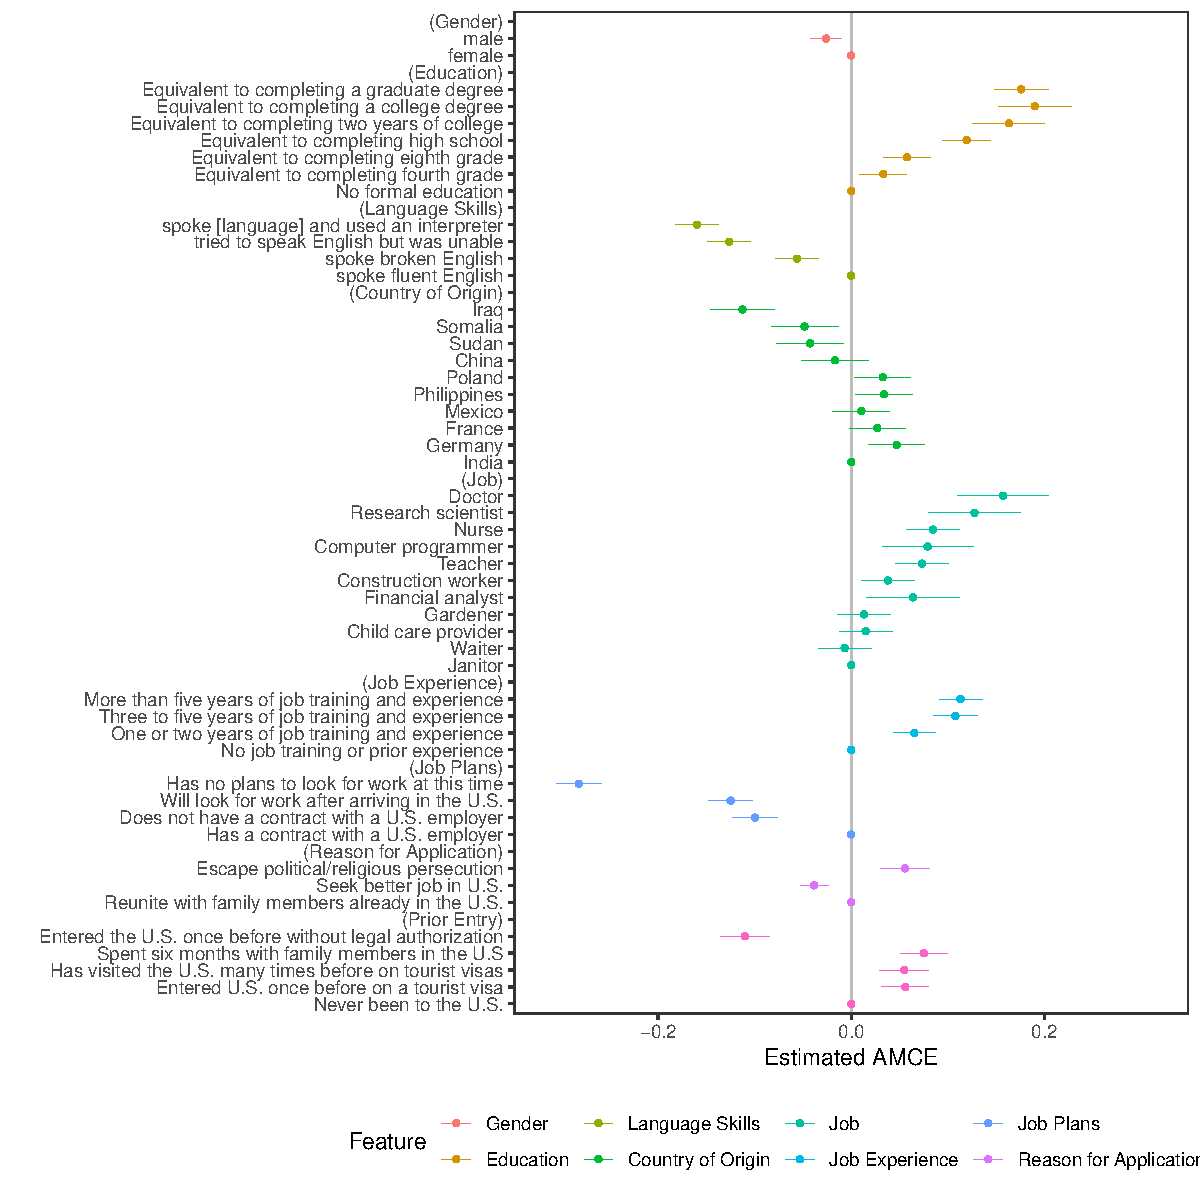
\includegraphics[width=\maxwidth]{figure/hainmueller_immigration_amce_appendix-1} 

\end{knitrout}

\clearpage

\begin{knitrout}
\definecolor{shadecolor}{rgb}{0.969, 0.969, 0.969}\color{fgcolor}
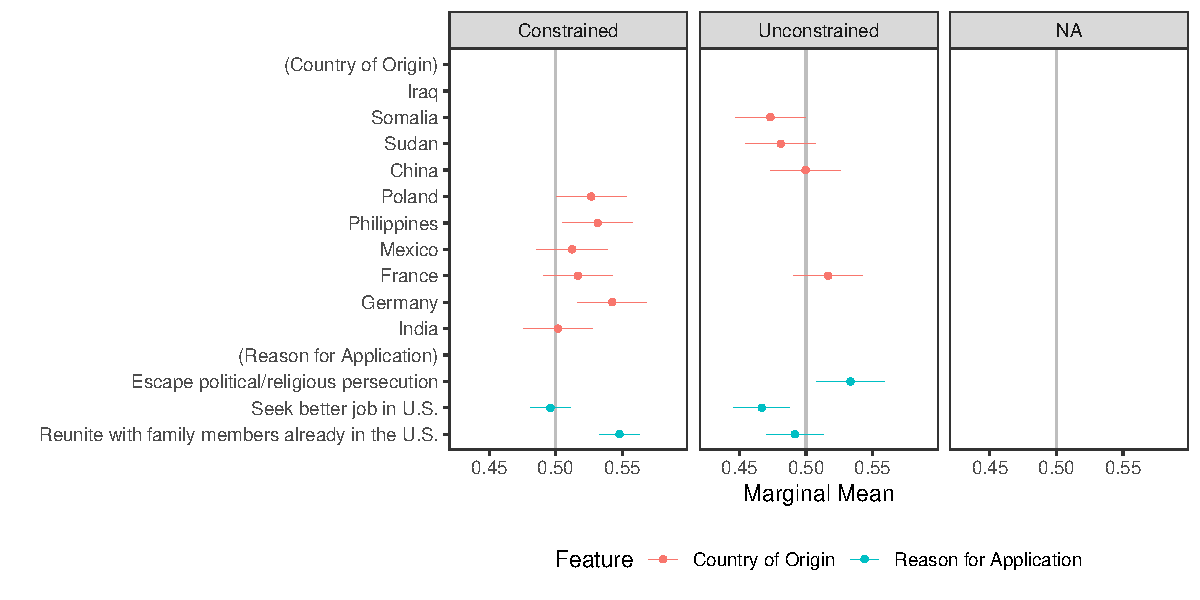
\includegraphics[width=\maxwidth]{figure/hainmueller_immigration_amce_appendix_split-1} 

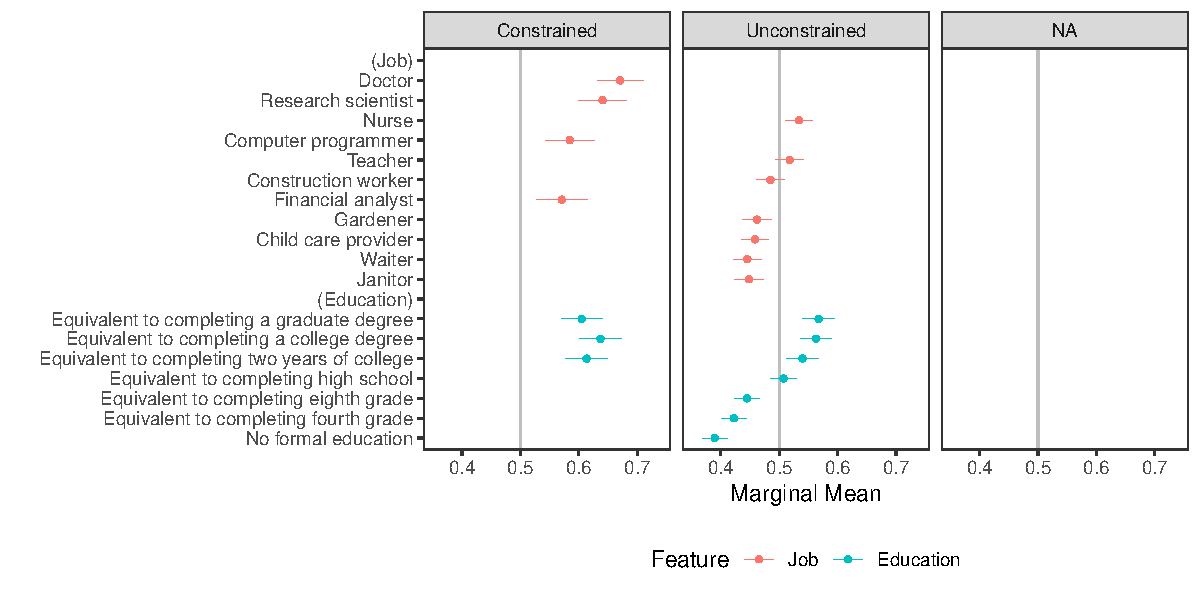
\includegraphics[width=\maxwidth]{figure/hainmueller_immigration_amce_appendix_split-2} 

\end{knitrout}

\clearpage

% latex table generated in R 3.5.2 by xtable 1.8-3 package
% Fri Mar 15 15:56:01 2019
\begin{table}[ht]
\centering
\begingroup\footnotesize
\begin{tabular}{lp{3in}rrr}
  \hline
feature & level & estimate & std.error & z \\ 
  \hline
Gender & female & 0.00 &  &  \\ 
  Gender & male & -0.03 & 0.01 & -3.25 \\ 
  Education & No formal education & 0.00 &  &  \\ 
  Education & Equivalent to completing fourth grade & 0.03 & 0.01 & 2.22 \\ 
  Education & Equivalent to completing eighth grade & 0.06 & 0.01 & 3.86 \\ 
  Education & Equivalent to completing high school & 0.12 & 0.01 & 7.98 \\ 
  Education & Equivalent to completing two years of college & 0.16 & 0.02 & 7.12 \\ 
  Education & Equivalent to completing a college degree & 0.19 & 0.02 & 8.26 \\ 
  Education & Equivalent to completing a graduate degree & 0.18 & 0.02 & 10.41 \\ 
  Language Skills & spoke fluent English & 0.00 &  &  \\ 
  Language Skills & spoke broken English & -0.06 & 0.01 & -4.98 \\ 
  Language Skills & tried to speak English but was unable & -0.13 & 0.01 & -11.11 \\ 
  Language Skills & spoke [language] and used an interpreter & -0.16 & 0.01 & -13.78 \\ 
  Country of Origin & India & 0.00 &  &  \\ 
  Country of Origin & Germany & 0.05 & 0.02 & 2.66 \\ 
  Country of Origin & France & 0.03 & 0.02 & 1.53 \\ 
  Country of Origin & Mexico & 0.01 & 0.02 & 0.59 \\ 
  Country of Origin & Philippines & 0.03 & 0.02 & 1.91 \\ 
  Country of Origin & Poland & 0.03 & 0.02 & 1.83 \\ 
  Country of Origin & China & -0.02 & 0.02 & -0.81 \\ 
  Country of Origin & Sudan & -0.04 & 0.02 & -2.01 \\ 
  Country of Origin & Somalia & -0.05 & 0.02 & -2.29 \\ 
  Country of Origin & Iraq & -0.11 & 0.02 & -5.56 \\ 
  Job & Janitor & 0.00 &  &  \\ 
  Job & Waiter & -0.01 & 0.02 & -0.41 \\ 
  Job & Child care provider & 0.01 & 0.02 & 0.89 \\ 
  Job & Gardener & 0.01 & 0.02 & 0.78 \\ 
  Job & Financial analyst & 0.06 & 0.03 & 2.17 \\ 
  Job & Construction worker & 0.04 & 0.02 & 2.26 \\ 
  Job & Teacher & 0.07 & 0.02 & 4.39 \\ 
  Job & Computer programmer & 0.08 & 0.03 & 2.76 \\ 
  Job & Nurse & 0.08 & 0.02 & 5.08 \\ 
  Job & Research scientist & 0.13 & 0.03 & 4.44 \\ 
  Job & Doctor & 0.16 & 0.03 & 5.49 \\ 
  Job Experience & No job training or prior experience & 0.00 &  &  \\ 
  Job Experience & One or two years of job training and experience & 0.07 & 0.01 & 5.92 \\ 
  Job Experience & Three to five years of job training and experience & 0.11 & 0.01 & 9.32 \\ 
  Job Experience & More than five years of job training and experience & 0.11 & 0.01 & 9.96 \\ 
  Job Plans & Has a contract with a U.S. employer & 0.00 &  &  \\ 
  Job Plans & Does not have a contract with a U.S. employer & -0.10 & 0.01 & -8.50 \\ 
  Job Plans & Will look for work after arriving in the U.S. & -0.12 & 0.01 & -10.69 \\ 
  Job Plans & Has no plans to look for work at this time & -0.28 & 0.01 & -23.91 \\ 
  Reason for Application & Reunite with family members already in the U.S. & 0.00 &  &  \\ 
  Reason for Application & Seek better job in U.S. & -0.04 & 0.01 & -4.37 \\ 
  Reason for Application & Escape political/religious persecution & 0.06 & 0.02 & 3.58 \\ 
  Prior Entry & Never been to the U.S. & 0.00 &  &  \\ 
  Prior Entry & Entered U.S. once before on a tourist visa & 0.06 & 0.01 & 4.49 \\ 
  Prior Entry & Has visited the U.S. many times before on tourist visas & 0.05 & 0.01 & 4.24 \\ 
  Prior Entry & Spent six months with family members in the U.S & 0.08 & 0.01 & 5.98 \\ 
  Prior Entry & Entered the U.S. once before without legal authorization & -0.11 & 0.01 & -8.45 \\ 
   \hline
\end{tabular}
\endgroup
\end{table}


\clearpage

\subsection{Replication using MMs}

\begin{knitrout}
\definecolor{shadecolor}{rgb}{0.969, 0.969, 0.969}\color{fgcolor}
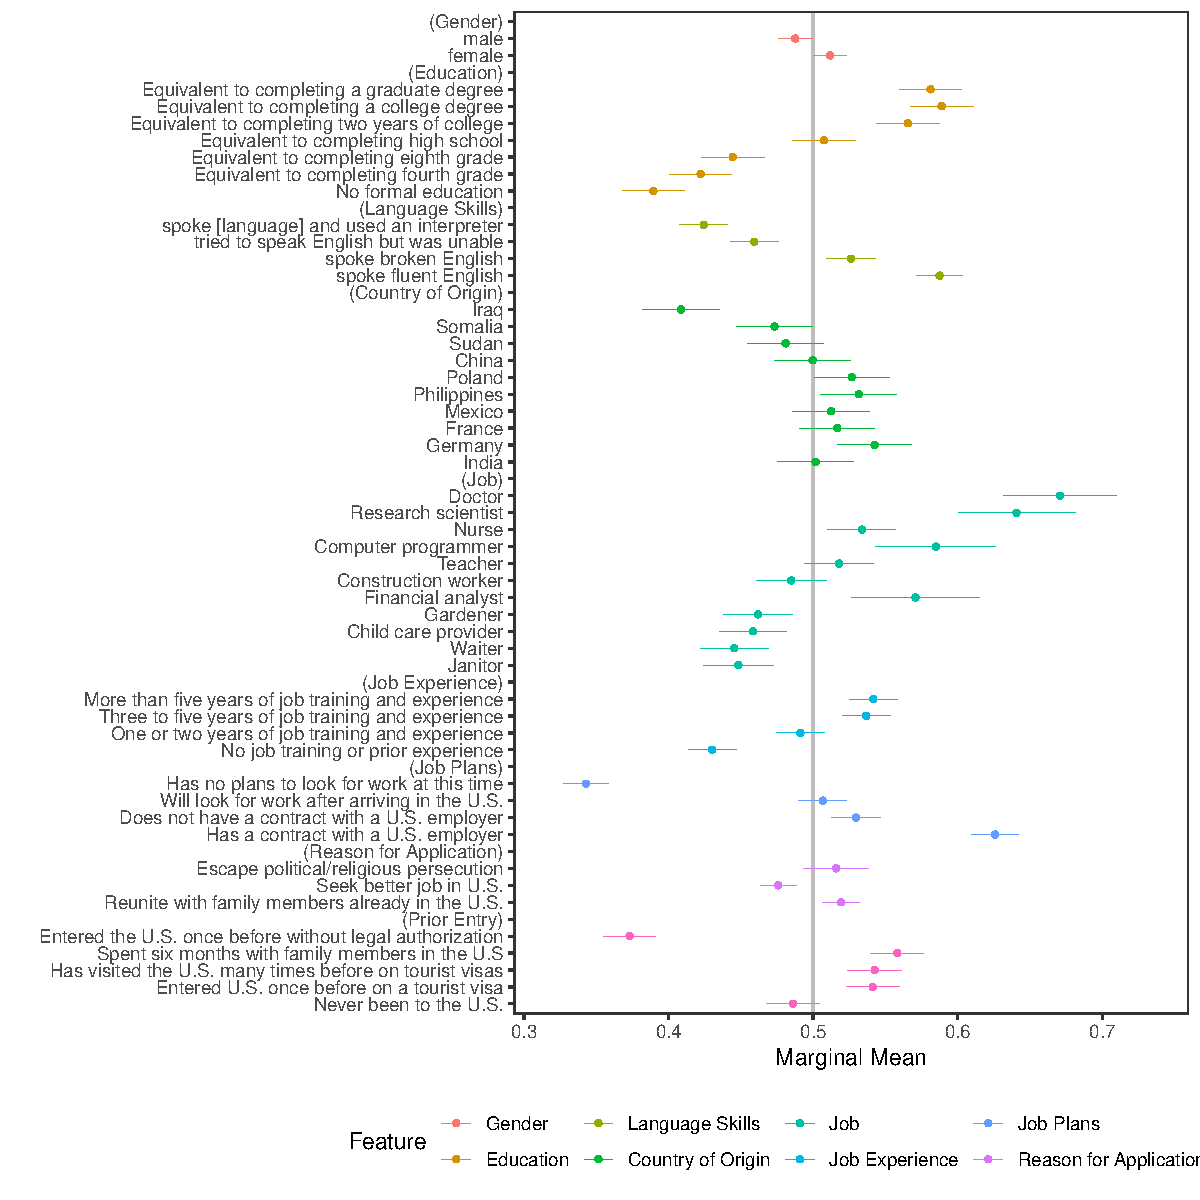
\includegraphics[width=\maxwidth]{figure/hainmueller_immigration_mm_appendix-1} 

\end{knitrout}

\clearpage

% latex table generated in R 3.5.2 by xtable 1.8-3 package
% Fri Mar 15 15:56:08 2019
\begin{table}[ht]
\centering
\begingroup\footnotesize
\begin{tabular}{lp{3in}rrr}
  \hline
feature & level & estimate & std.error & z \\ 
  \hline
Gender & female & 0.51 & 0.01 & 1.99 \\ 
  Gender & male & 0.49 & 0.01 & -2.03 \\ 
  Education & No formal education & 0.39 & 0.01 & -10.04 \\ 
  Education & Equivalent to completing fourth grade & 0.42 & 0.01 & -7.08 \\ 
  Education & Equivalent to completing eighth grade & 0.44 & 0.01 & -5.00 \\ 
  Education & Equivalent to completing high school & 0.51 & 0.01 & 0.67 \\ 
  Education & Equivalent to completing two years of college & 0.57 & 0.01 & 5.92 \\ 
  Education & Equivalent to completing a college degree & 0.59 & 0.01 & 8.00 \\ 
  Education & Equivalent to completing a graduate degree & 0.58 & 0.01 & 7.40 \\ 
  Language Skills & spoke fluent English & 0.59 & 0.01 & 10.63 \\ 
  Language Skills & spoke broken English & 0.53 & 0.01 & 3.07 \\ 
  Language Skills & tried to speak English but was unable & 0.46 & 0.01 & -4.83 \\ 
  Language Skills & spoke [language] and used an interpreter & 0.42 & 0.01 & -8.98 \\ 
  Country of Origin & India & 0.50 & 0.01 & 0.13 \\ 
  Country of Origin & Germany & 0.54 & 0.01 & 3.22 \\ 
  Country of Origin & France & 0.52 & 0.01 & 1.26 \\ 
  Country of Origin & Mexico & 0.51 & 0.01 & 0.92 \\ 
  Country of Origin & Philippines & 0.53 & 0.01 & 2.36 \\ 
  Country of Origin & Poland & 0.53 & 0.01 & 2.01 \\ 
  Country of Origin & China & 0.50 & 0.01 & -0.03 \\ 
  Country of Origin & Sudan & 0.48 & 0.01 & -1.42 \\ 
  Country of Origin & Somalia & 0.47 & 0.01 & -2.01 \\ 
  Country of Origin & Iraq & 0.41 & 0.01 & -6.76 \\ 
  Job & Janitor & 0.45 & 0.01 & -4.20 \\ 
  Job & Waiter & 0.45 & 0.01 & -4.56 \\ 
  Job & Child care provider & 0.46 & 0.01 & -3.50 \\ 
  Job & Gardener & 0.46 & 0.01 & -3.11 \\ 
  Job & Financial analyst & 0.57 & 0.02 & 3.16 \\ 
  Job & Construction worker & 0.48 & 0.01 & -1.23 \\ 
  Job & Teacher & 0.52 & 0.01 & 1.49 \\ 
  Job & Computer programmer & 0.58 & 0.02 & 4.01 \\ 
  Job & Nurse & 0.53 & 0.01 & 2.82 \\ 
  Job & Research scientist & 0.64 & 0.02 & 6.82 \\ 
  Job & Doctor & 0.67 & 0.02 & 8.53 \\ 
  Job Experience & No job training or prior experience & 0.43 & 0.01 & -8.27 \\ 
  Job Experience & One or two years of job training and experience & 0.49 & 0.01 & -1.05 \\ 
  Job Experience & Three to five years of job training and experience & 0.54 & 0.01 & 4.33 \\ 
  Job Experience & More than five years of job training and experience & 0.54 & 0.01 & 4.92 \\ 
  Job Plans & Has a contract with a U.S. employer & 0.63 & 0.01 & 15.40 \\ 
  Job Plans & Does not have a contract with a U.S. employer & 0.53 & 0.01 & 3.47 \\ 
  Job Plans & Will look for work after arriving in the U.S. & 0.51 & 0.01 & 0.78 \\ 
  Job Plans & Has no plans to look for work at this time & 0.34 & 0.01 & -19.86 \\ 
  Reason for Application & Reunite with family members already in the U.S. & 0.52 & 0.01 & 3.00 \\ 
  Reason for Application & Seek better job in U.S. & 0.48 & 0.01 & -3.76 \\ 
  Reason for Application & Escape political/religious persecution & 0.52 & 0.01 & 1.40 \\ 
  Prior Entry & Never been to the U.S. & 0.49 & 0.01 & -1.47 \\ 
  Prior Entry & Entered U.S. once before on a tourist visa & 0.54 & 0.01 & 4.37 \\ 
  Prior Entry & Has visited the U.S. many times before on tourist visas & 0.54 & 0.01 & 4.50 \\ 
  Prior Entry & Spent six months with family members in the U.S & 0.56 & 0.01 & 6.24 \\ 
  Prior Entry & Entered the U.S. once before without legal authorization & 0.37 & 0.01 & -13.96 \\ 
   \hline
\end{tabular}
\endgroup
\end{table}


\clearpage

\subsection{Subgroup Analysis for Hainmueller et al. (2014) Immigration Experiment using AMCEs}

\begin{knitrout}
\definecolor{shadecolor}{rgb}{0.969, 0.969, 0.969}\color{fgcolor}
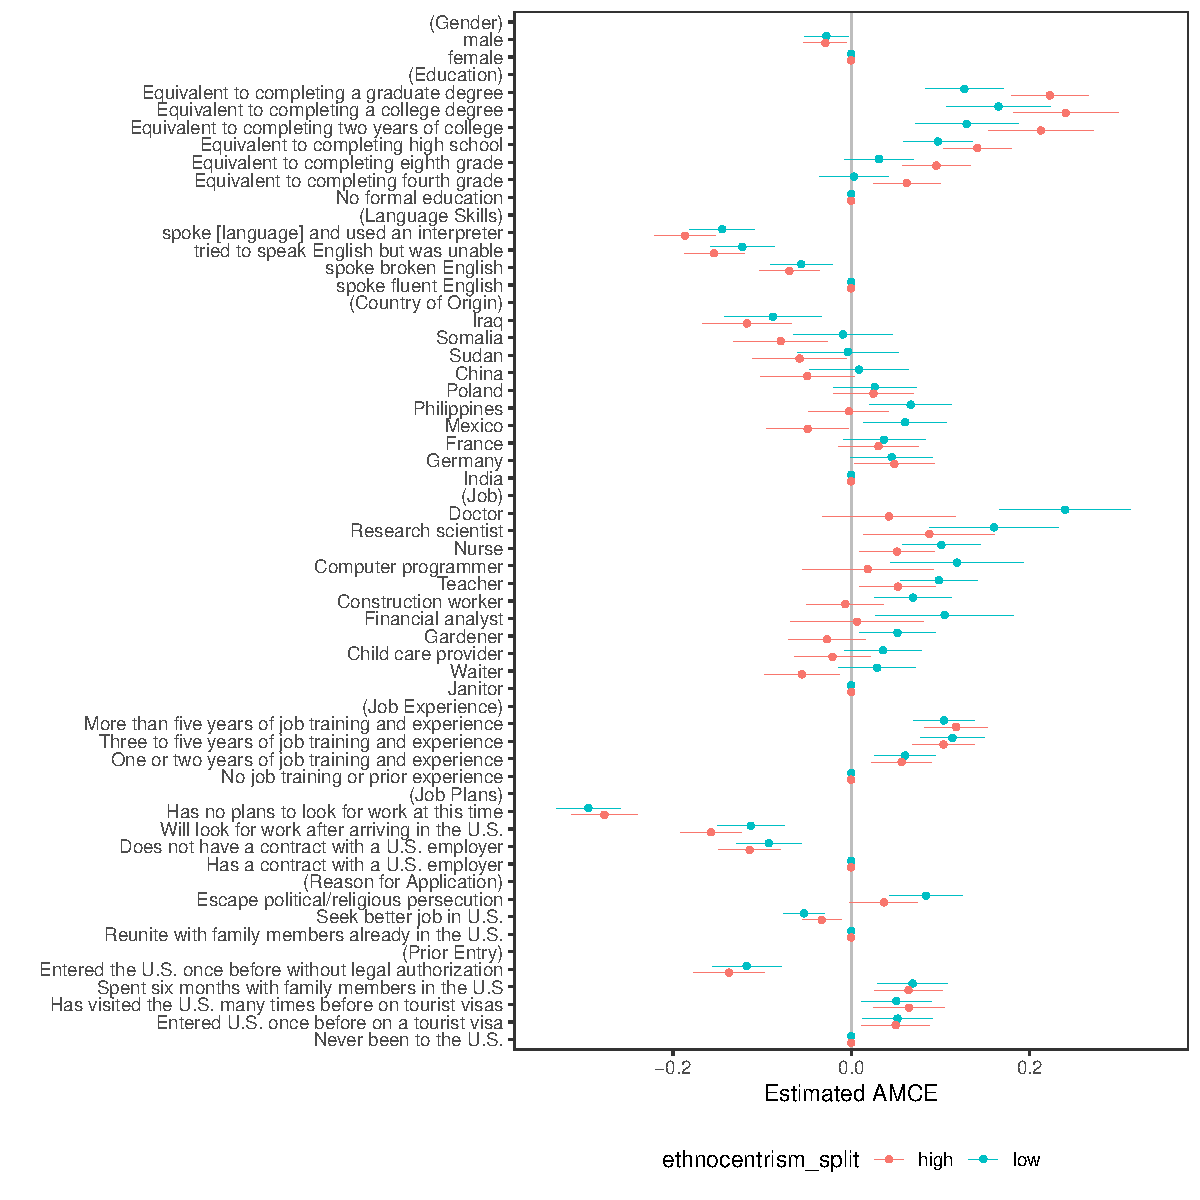
\includegraphics[width=\maxwidth]{figure/hainmueller_immigration_subgroup_amce_appendix-1} 

\end{knitrout}

\clearpage

\subsection{Subgroup Analysis for Hainmueller et al. (2014) Immigration Experiment using MMs}

\begin{knitrout}
\definecolor{shadecolor}{rgb}{0.969, 0.969, 0.969}\color{fgcolor}
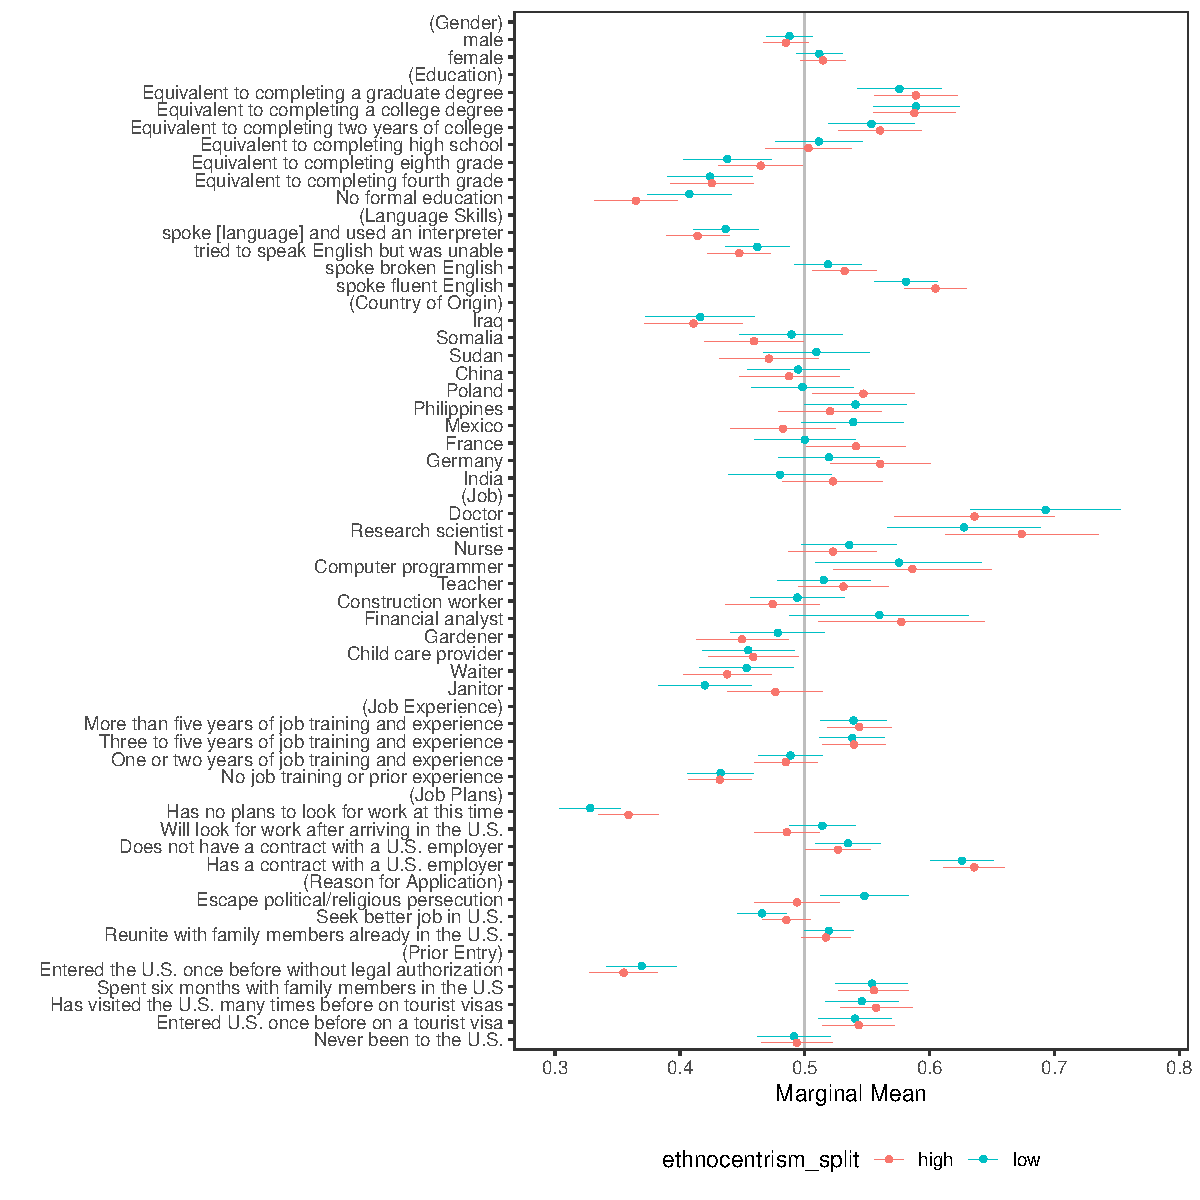
\includegraphics[width=\maxwidth]{figure/hainmueller_immigration_subgroup_mm_appendix-1} 

\end{knitrout}

\clearpage


\section{Hainmueller et al. (2014) Candidate Experiment}

\subsection{Replication using AMCEs}

\begin{knitrout}
\definecolor{shadecolor}{rgb}{0.969, 0.969, 0.969}\color{fgcolor}
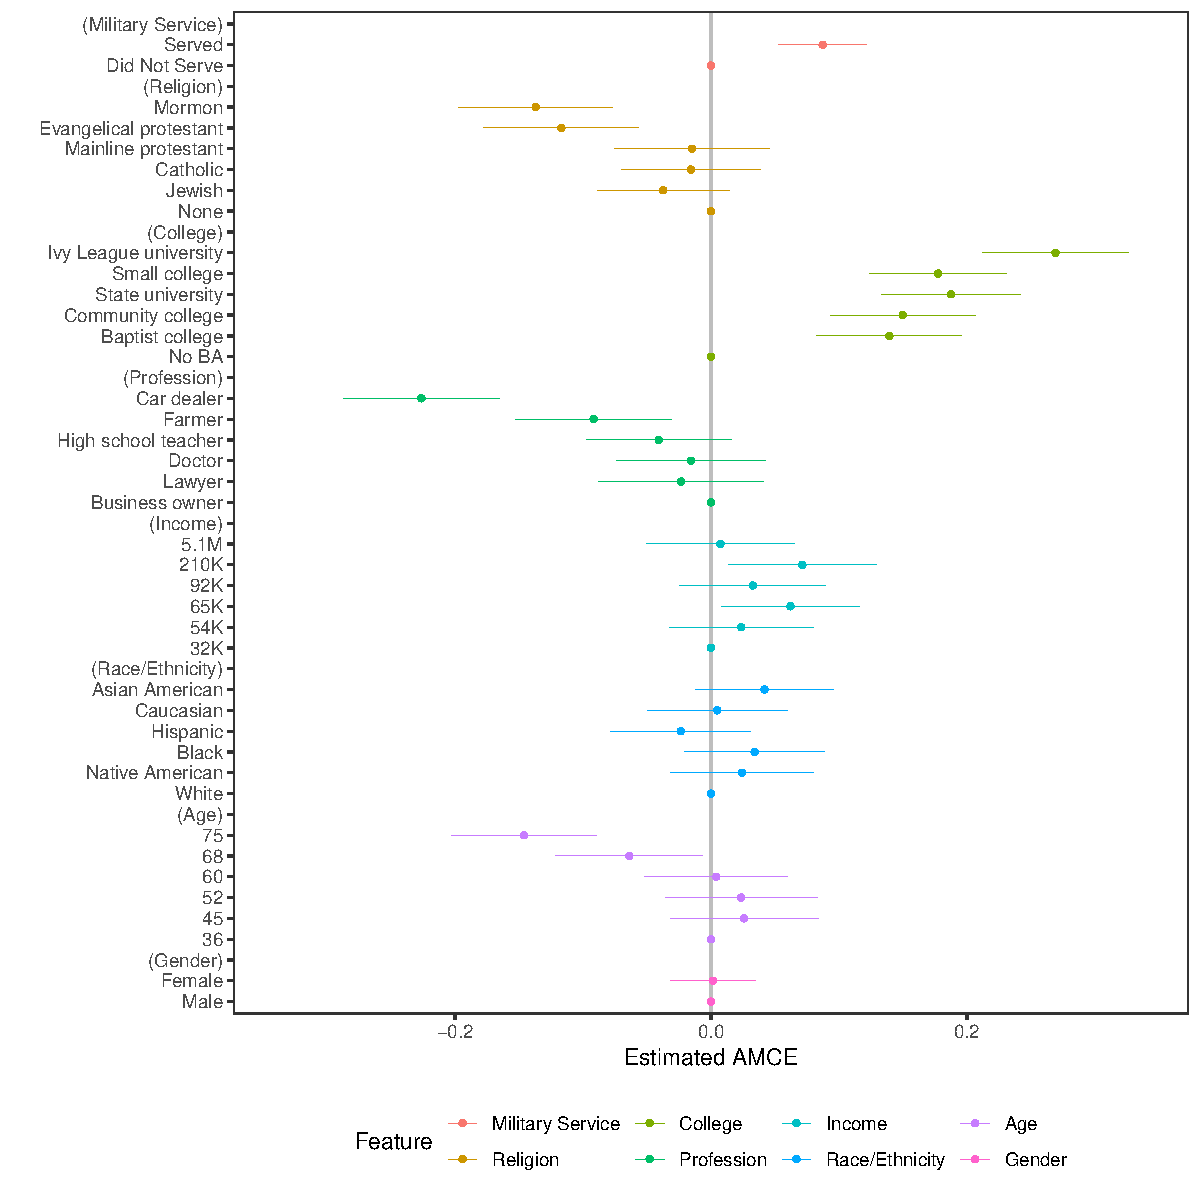
\includegraphics[width=\maxwidth]{figure/hainmueller_candidate_amce_appendix-1} 

\end{knitrout}

\clearpage

% latex table generated in R 3.5.1 by xtable 1.8-3 package
% Sun Nov 25 10:42:42 2018
\begin{table}[ht]
\centering
\begingroup\footnotesize
\begin{tabular}{lp{3in}rrr}
  \hline
feature & level & estimate & std.error & z \\ 
  \hline
Military Service & Did Not Serve & 0.00 &  &  \\ 
  Military Service & Served & 0.09 & 0.02 & 4.95 \\ 
  Religion & None & 0.00 &  &  \\ 
  Religion & Jewish & -0.04 & 0.03 & -1.42 \\ 
  Religion & Catholic & -0.02 & 0.03 & -0.56 \\ 
  Religion & Mainline protestant & -0.01 & 0.03 & -0.48 \\ 
  Religion & Evangelical protestant & -0.12 & 0.03 & -3.78 \\ 
  Religion & Mormon & -0.14 & 0.03 & -4.46 \\ 
  College & No BA & 0.00 &  &  \\ 
  College & Baptist college & 0.14 & 0.03 & 4.82 \\ 
  College & Community college & 0.15 & 0.03 & 5.17 \\ 
  College & State university & 0.19 & 0.03 & 6.77 \\ 
  College & Small college & 0.18 & 0.03 & 6.50 \\ 
  College & Ivy League university & 0.27 & 0.03 & 9.26 \\ 
  Profession & Business owner & 0.00 &  &  \\ 
  Profession & Lawyer & -0.02 & 0.03 & -0.71 \\ 
  Profession & Doctor & -0.02 & 0.03 & -0.53 \\ 
  Profession & High school teacher & -0.04 & 0.03 & -1.42 \\ 
  Profession & Farmer & -0.09 & 0.03 & -2.94 \\ 
  Profession & Car dealer & -0.23 & 0.03 & -7.24 \\ 
  Income & 32K & 0.00 &  &  \\ 
  Income & 54K & 0.02 & 0.03 & 0.82 \\ 
  Income & 65K & 0.06 & 0.03 & 2.26 \\ 
  Income & 92K & 0.03 & 0.03 & 1.12 \\ 
  Income & 210K & 0.07 & 0.03 & 2.41 \\ 
  Income & 5.1M & 0.01 & 0.03 & 0.25 \\ 
  Race/Ethnicity & White & 0.00 &  &  \\ 
  Race/Ethnicity & Native American & 0.02 & 0.03 & 0.85 \\ 
  Race/Ethnicity & Black & 0.03 & 0.03 & 1.22 \\ 
  Race/Ethnicity & Hispanic & -0.02 & 0.03 & -0.84 \\ 
  Race/Ethnicity & Caucasian & 0.00 & 0.03 & 0.18 \\ 
  Race/Ethnicity & Asian American & 0.04 & 0.03 & 1.51 \\ 
  Age & 36 & 0.00 &  &  \\ 
  Age & 45 & 0.03 & 0.03 & 0.88 \\ 
  Age & 52 & 0.02 & 0.03 & 0.78 \\ 
  Age & 60 & 0.00 & 0.03 & 0.14 \\ 
  Age & 68 & -0.06 & 0.03 & -2.17 \\ 
  Age & 75 & -0.15 & 0.03 & -5.06 \\ 
  Gender & Male & 0.00 &  &  \\ 
  Gender & Female & 0.00 & 0.02 & 0.09 \\ 
   \hline
\end{tabular}
\endgroup
\end{table}


\clearpage

\subsection{Replication using MMs}

\begin{knitrout}
\definecolor{shadecolor}{rgb}{0.969, 0.969, 0.969}\color{fgcolor}
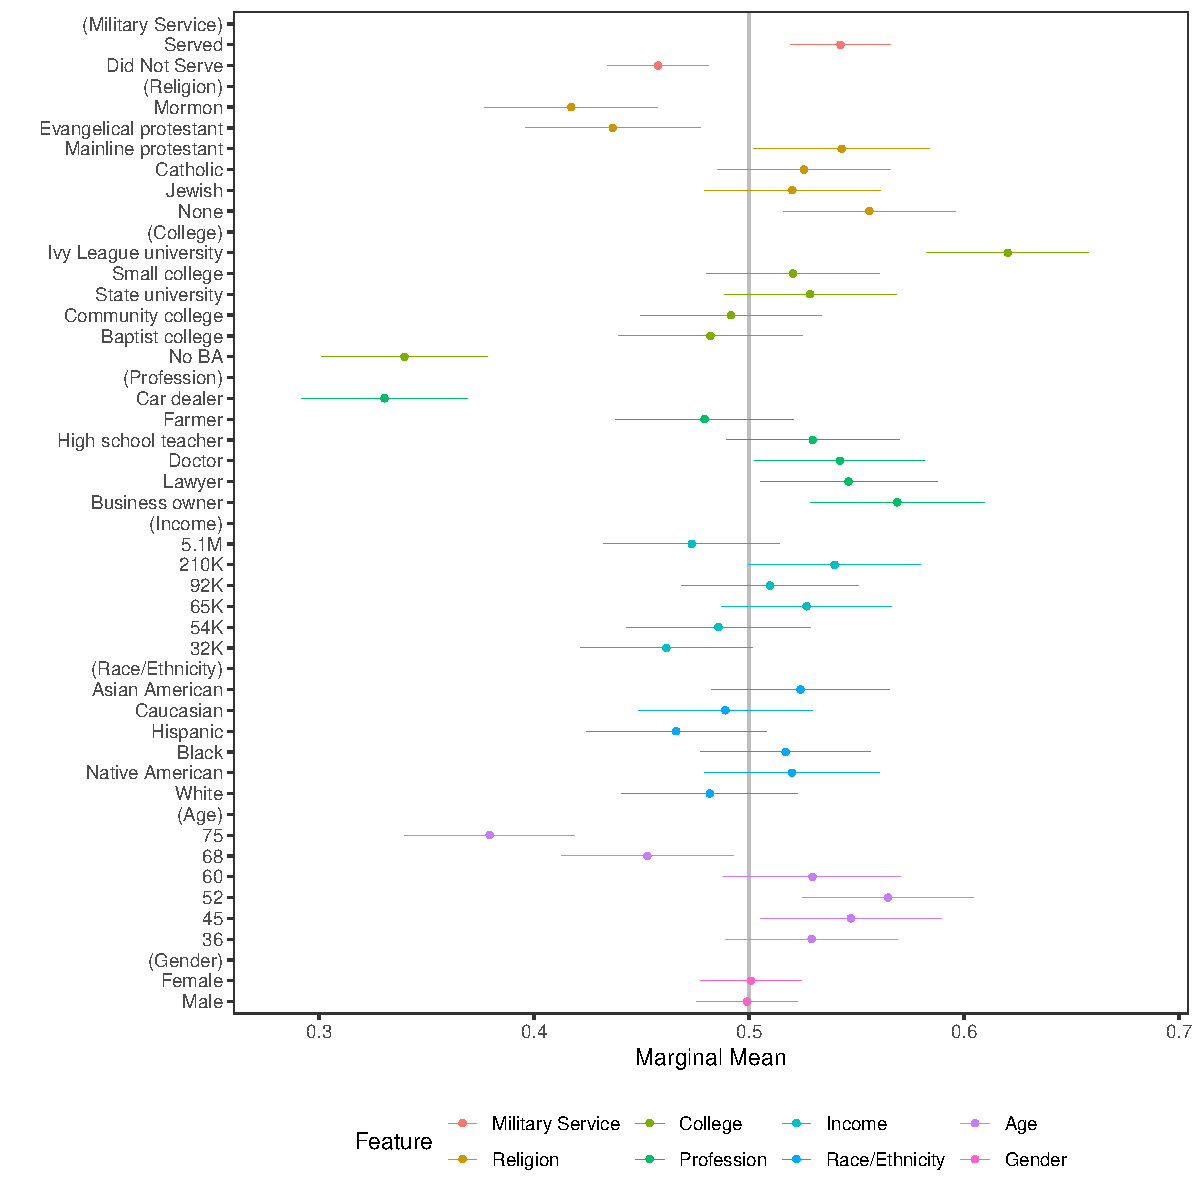
\includegraphics[width=\maxwidth]{figure/hainmueller_candidate_mm_appendix-1} 

\end{knitrout}

\clearpage

% latex table generated in R 3.5.1 by xtable 1.8-3 package
% Sun Nov 25 10:42:44 2018
\begin{table}[ht]
\centering
\begingroup\footnotesize
\begin{tabular}{lp{3in}rrr}
  \hline
feature & level & estimate & std.error & z \\ 
  \hline
Military Service & Did Not Serve & 0.46 & 0.01 & -3.54 \\ 
  Military Service & Served & 0.54 & 0.01 & 3.55 \\ 
  Religion & None & 0.56 & 0.02 & 2.73 \\ 
  Religion & Jewish & 0.52 & 0.02 & 0.96 \\ 
  Religion & Catholic & 0.53 & 0.02 & 1.24 \\ 
  Religion & Mainline protestant & 0.54 & 0.02 & 2.06 \\ 
  Religion & Evangelical protestant & 0.44 & 0.02 & -3.05 \\ 
  Religion & Mormon & 0.42 & 0.02 & -4.04 \\ 
  College & No BA & 0.34 & 0.02 & -8.11 \\ 
  College & Baptist college & 0.48 & 0.02 & -0.83 \\ 
  College & Community college & 0.49 & 0.02 & -0.39 \\ 
  College & State university & 0.53 & 0.02 & 1.39 \\ 
  College & Small college & 0.52 & 0.02 & 0.99 \\ 
  College & Ivy League university & 0.62 & 0.02 & 6.27 \\ 
  Profession & Business owner & 0.57 & 0.02 & 3.35 \\ 
  Profession & Lawyer & 0.55 & 0.02 & 2.20 \\ 
  Profession & Doctor & 0.54 & 0.02 & 2.08 \\ 
  Profession & High school teacher & 0.53 & 0.02 & 1.44 \\ 
  Profession & Farmer & 0.48 & 0.02 & -0.98 \\ 
  Profession & Car dealer & 0.33 & 0.02 & -8.64 \\ 
  Income & 32K & 0.46 & 0.02 & -1.89 \\ 
  Income & 54K & 0.49 & 0.02 & -0.65 \\ 
  Income & 65K & 0.53 & 0.02 & 1.33 \\ 
  Income & 92K & 0.51 & 0.02 & 0.46 \\ 
  Income & 210K & 0.54 & 0.02 & 1.94 \\ 
  Income & 5.1M & 0.47 & 0.02 & -1.26 \\ 
  Race/Ethnicity & White & 0.48 & 0.02 & -0.88 \\ 
  Race/Ethnicity & Native American & 0.52 & 0.02 & 0.96 \\ 
  Race/Ethnicity & Black & 0.52 & 0.02 & 0.85 \\ 
  Race/Ethnicity & Hispanic & 0.47 & 0.02 & -1.59 \\ 
  Race/Ethnicity & Caucasian & 0.49 & 0.02 & -0.53 \\ 
  Race/Ethnicity & Asian American & 0.52 & 0.02 & 1.14 \\ 
  Age & 36 & 0.53 & 0.02 & 1.43 \\ 
  Age & 45 & 0.55 & 0.02 & 2.21 \\ 
  Age & 52 & 0.56 & 0.02 & 3.18 \\ 
  Age & 60 & 0.53 & 0.02 & 1.40 \\ 
  Age & 68 & 0.45 & 0.02 & -2.31 \\ 
  Age & 75 & 0.38 & 0.02 & -5.99 \\ 
  Gender & Male & 0.50 & 0.01 & -0.07 \\ 
  Gender & Female & 0.50 & 0.01 & 0.07 \\ 
   \hline
\end{tabular}
\endgroup
\end{table}


\clearpage

\section{Ballard-Rosa et al. (2016) Tax Preference Experiment}

\subsection{Replication using AMCEs}

\begin{knitrout}
\definecolor{shadecolor}{rgb}{0.969, 0.969, 0.969}\color{fgcolor}
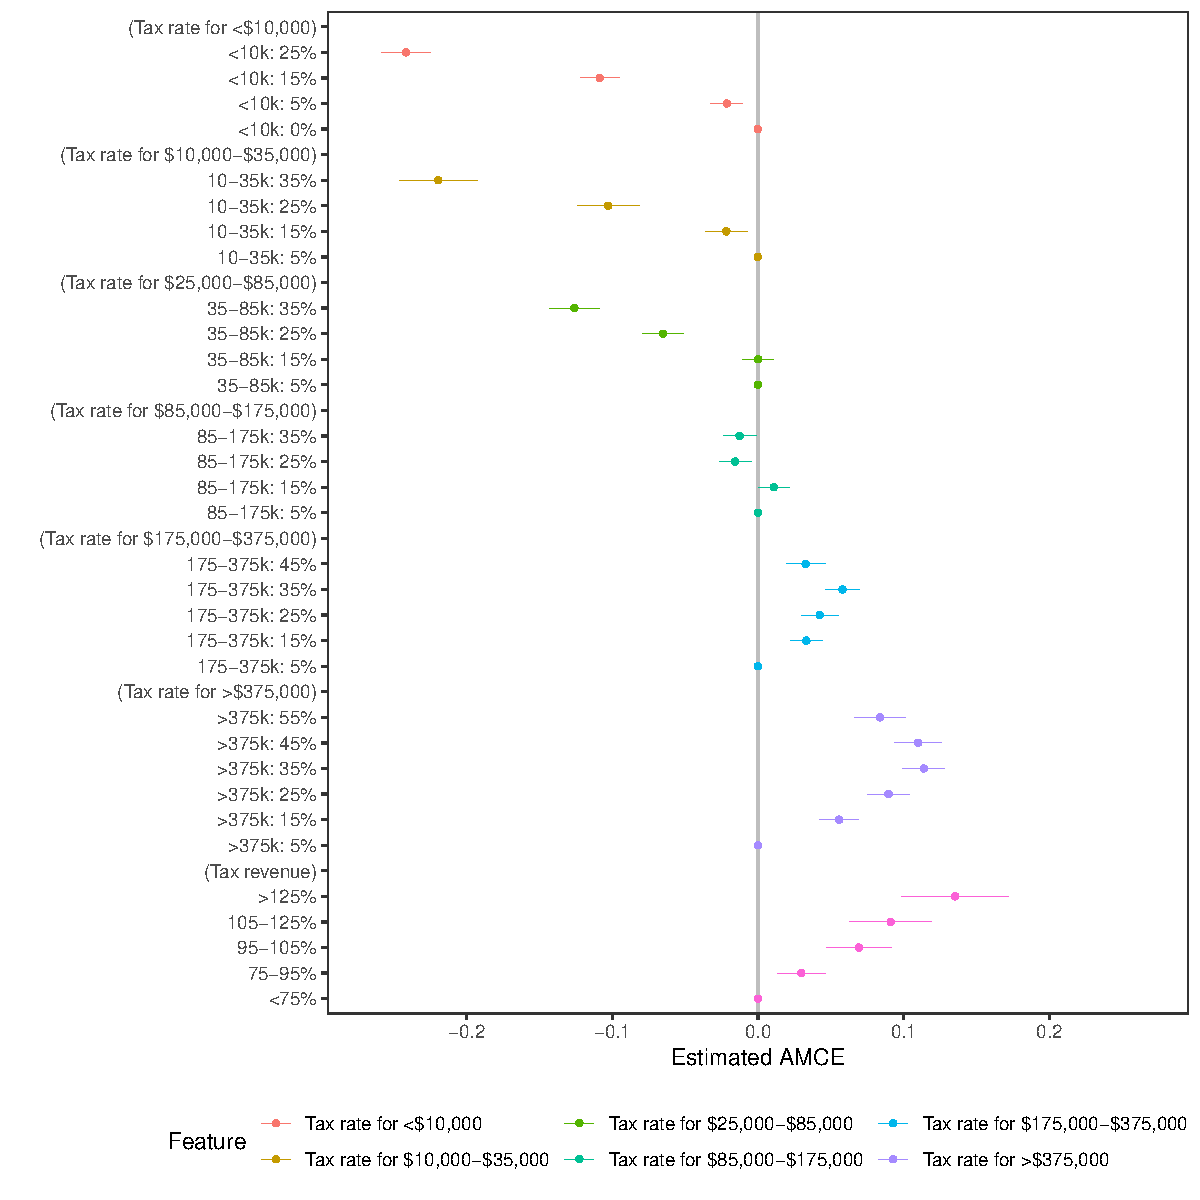
\includegraphics[width=\maxwidth]{figure/bms_amce_appendix-1} 

\end{knitrout}

\clearpage

% latex table generated in R 3.5.1 by xtable 1.8-3 package
% Sun Nov 25 10:42:47 2018
\begin{table}[ht]
\centering
\begin{tabular}{lp{1.5in}rrr}
  \hline
feature & level & estimate & std.error & z \\ 
  \hline
Tax rate for $<$\$10,000 & $<$10k: 0\% & 0.00 &  &  \\ 
  Tax rate for $<$\$10,000 & $<$10k: 5\% & -0.02 & 0.01 & -3.81 \\ 
  Tax rate for $<$\$10,000 & $<$10k: 15\% & -0.11 & 0.01 & -15.97 \\ 
  Tax rate for $<$\$10,000 & $<$10k: 25\% & -0.24 & 0.01 & -28.33 \\ 
  Tax rate for \$10,000-\$35,000 & 10-35k: 5\% & 0.00 &  &  \\ 
  Tax rate for \$10,000-\$35,000 & 10-35k: 15\% & -0.02 & 0.01 & -2.94 \\ 
  Tax rate for \$10,000-\$35,000 & 10-35k: 25\% & -0.10 & 0.01 & -9.42 \\ 
  Tax rate for \$10,000-\$35,000 & 10-35k: 35\% & -0.22 & 0.01 & -15.96 \\ 
  Tax rate for \$25,000-\$85,000 & 35-85k: 5\% & 0.00 &  &  \\ 
  Tax rate for \$25,000-\$85,000 & 35-85k: 15\% & 0.00 & 0.01 & 0.03 \\ 
  Tax rate for \$25,000-\$85,000 & 35-85k: 25\% & -0.07 & 0.01 & -9.18 \\ 
  Tax rate for \$25,000-\$85,000 & 35-85k: 35\% & -0.13 & 0.01 & -14.55 \\ 
  Tax rate for \$85,000-\$175,000 & 85-175k: 5\% & 0.00 &  &  \\ 
  Tax rate for \$85,000-\$175,000 & 85-175k: 15\% & 0.01 & 0.01 & 2.06 \\ 
  Tax rate for \$85,000-\$175,000 & 85-175k: 25\% & -0.02 & 0.01 & -2.80 \\ 
  Tax rate for \$85,000-\$175,000 & 85-175k: 35\% & -0.01 & 0.01 & -2.19 \\ 
  Tax rate for \$175,000-\$375,000 & 175-375k: 5\% & 0.00 &  &  \\ 
  Tax rate for \$175,000-\$375,000 & 175-375k: 15\% & 0.03 & 0.01 & 5.97 \\ 
  Tax rate for \$175,000-\$375,000 & 175-375k: 25\% & 0.04 & 0.01 & 6.53 \\ 
  Tax rate for \$175,000-\$375,000 & 175-375k: 35\% & 0.06 & 0.01 & 9.77 \\ 
  Tax rate for \$175,000-\$375,000 & 175-375k: 45\% & 0.03 & 0.01 & 4.80 \\ 
  Tax rate for $>$\$375,000 & $>$375k: 5\% & 0.00 &  &  \\ 
  Tax rate for $>$\$375,000 & $>$375k: 15\% & 0.06 & 0.01 & 8.22 \\ 
  Tax rate for $>$\$375,000 & $>$375k: 25\% & 0.09 & 0.01 & 12.18 \\ 
  Tax rate for $>$\$375,000 & $>$375k: 35\% & 0.11 & 0.01 & 15.44 \\ 
  Tax rate for $>$\$375,000 & $>$375k: 45\% & 0.11 & 0.01 & 13.23 \\ 
  Tax rate for $>$\$375,000 & $>$375k: 55\% & 0.08 & 0.01 & 9.55 \\ 
  Tax revenue & $<$75\% & 0.00 &  &  \\ 
  Tax revenue & 75-95\% & 0.03 & 0.01 & 3.56 \\ 
  Tax revenue & 95-105\% & 0.07 & 0.01 & 6.11 \\ 
  Tax revenue & 105-125\% & 0.09 & 0.01 & 6.33 \\ 
  Tax revenue & $>$125\% & 0.14 & 0.02 & 7.22 \\ 
   \hline
\end{tabular}
\end{table}


\clearpage

\subsection{Replication using MMs}

\begin{knitrout}
\definecolor{shadecolor}{rgb}{0.969, 0.969, 0.969}\color{fgcolor}
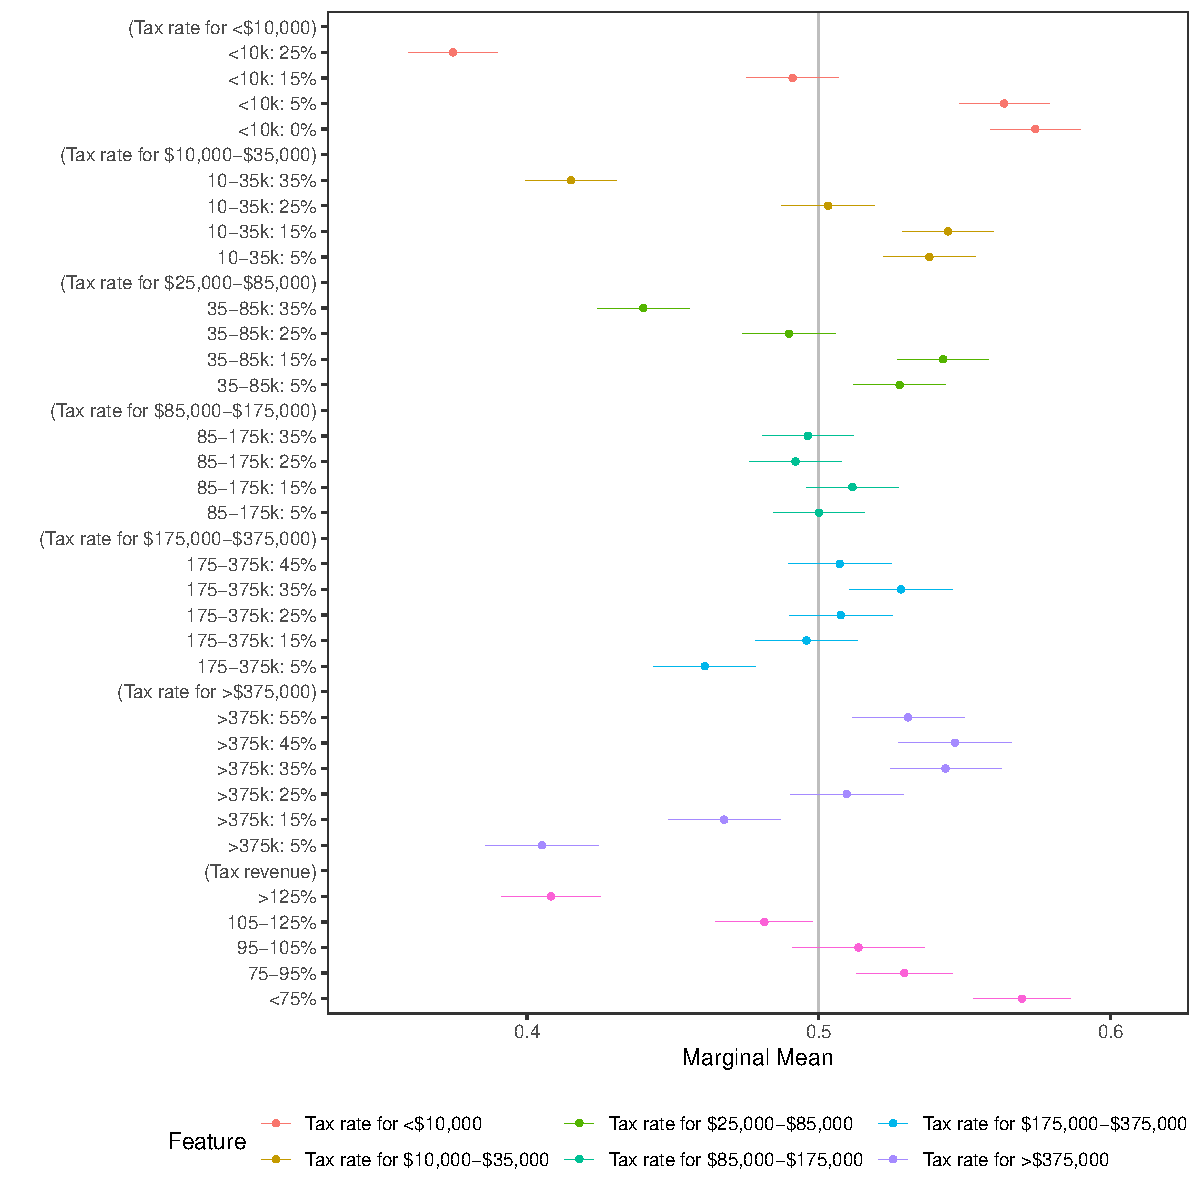
\includegraphics[width=\maxwidth]{figure/bms_mm_appendix-1} 

\end{knitrout}

\clearpage

% latex table generated in R 3.5.1 by xtable 1.8-3 package
% Sun Nov 25 10:42:56 2018
\begin{table}[ht]
\centering
\begin{tabular}{lp{1.5in}rrr}
  \hline
feature & level & estimate & std.error & z \\ 
  \hline
Tax rate for $<$\$10,000 & $<$10k: 0\% & 0.57 & 0.01 & 9.37 \\ 
  Tax rate for $<$\$10,000 & $<$10k: 5\% & 0.56 & 0.01 & 8.06 \\ 
  Tax rate for $<$\$10,000 & $<$10k: 15\% & 0.49 & 0.01 & -1.11 \\ 
  Tax rate for $<$\$10,000 & $<$10k: 25\% & 0.37 & 0.01 & -16.07 \\ 
  Tax rate for \$10,000-\$35,000 & 10-35k: 5\% & 0.54 & 0.01 & 4.75 \\ 
  Tax rate for \$10,000-\$35,000 & 10-35k: 15\% & 0.54 & 0.01 & 5.55 \\ 
  Tax rate for \$10,000-\$35,000 & 10-35k: 25\% & 0.50 & 0.01 & 0.39 \\ 
  Tax rate for \$10,000-\$35,000 & 10-35k: 35\% & 0.42 & 0.01 & -10.62 \\ 
  Tax rate for \$25,000-\$85,000 & 35-85k: 5\% & 0.53 & 0.01 & 3.45 \\ 
  Tax rate for \$25,000-\$85,000 & 35-85k: 15\% & 0.54 & 0.01 & 5.37 \\ 
  Tax rate for \$25,000-\$85,000 & 35-85k: 25\% & 0.49 & 0.01 & -1.27 \\ 
  Tax rate for \$25,000-\$85,000 & 35-85k: 35\% & 0.44 & 0.01 & -7.50 \\ 
  Tax rate for \$85,000-\$175,000 & 85-175k: 5\% & 0.50 & 0.01 & 0.00 \\ 
  Tax rate for \$85,000-\$175,000 & 85-175k: 15\% & 0.51 & 0.01 & 1.42 \\ 
  Tax rate for \$85,000-\$175,000 & 85-175k: 25\% & 0.49 & 0.01 & -1.00 \\ 
  Tax rate for \$85,000-\$175,000 & 85-175k: 35\% & 0.50 & 0.01 & -0.46 \\ 
  Tax rate for \$175,000-\$375,000 & 175-375k: 5\% & 0.46 & 0.01 & -4.37 \\ 
  Tax rate for \$175,000-\$375,000 & 175-375k: 15\% & 0.50 & 0.01 & -0.47 \\ 
  Tax rate for \$175,000-\$375,000 & 175-375k: 25\% & 0.51 & 0.01 & 0.84 \\ 
  Tax rate for \$175,000-\$375,000 & 175-375k: 35\% & 0.53 & 0.01 & 3.11 \\ 
  Tax rate for \$175,000-\$375,000 & 175-375k: 45\% & 0.51 & 0.01 & 0.80 \\ 
  Tax rate for $>$\$375,000 & $>$375k: 5\% & 0.41 & 0.01 & -9.57 \\ 
  Tax rate for $>$\$375,000 & $>$375k: 15\% & 0.47 & 0.01 & -3.30 \\ 
  Tax rate for $>$\$375,000 & $>$375k: 25\% & 0.51 & 0.01 & 0.97 \\ 
  Tax rate for $>$\$375,000 & $>$375k: 35\% & 0.54 & 0.01 & 4.48 \\ 
  Tax rate for $>$\$375,000 & $>$375k: 45\% & 0.55 & 0.01 & 4.75 \\ 
  Tax rate for $>$\$375,000 & $>$375k: 55\% & 0.53 & 0.01 & 3.12 \\ 
  Tax revenue & $<$75\% & 0.57 & 0.01 & 8.22 \\ 
  Tax revenue & 75-95\% & 0.53 & 0.01 & 3.47 \\ 
  Tax revenue & 95-105\% & 0.51 & 0.01 & 1.18 \\ 
  Tax revenue & 105-125\% & 0.48 & 0.01 & -2.21 \\ 
  Tax revenue & $>$125\% & 0.41 & 0.01 & -10.54 \\ 
   \hline
\end{tabular}
\end{table}


\clearpage

\subsection{Subgroup Analysis for Ballard-Rosa et al. (2016), by ``Taxes Harm Economy'' Split using AMCEs}

\begin{knitrout}
\definecolor{shadecolor}{rgb}{0.969, 0.969, 0.969}\color{fgcolor}
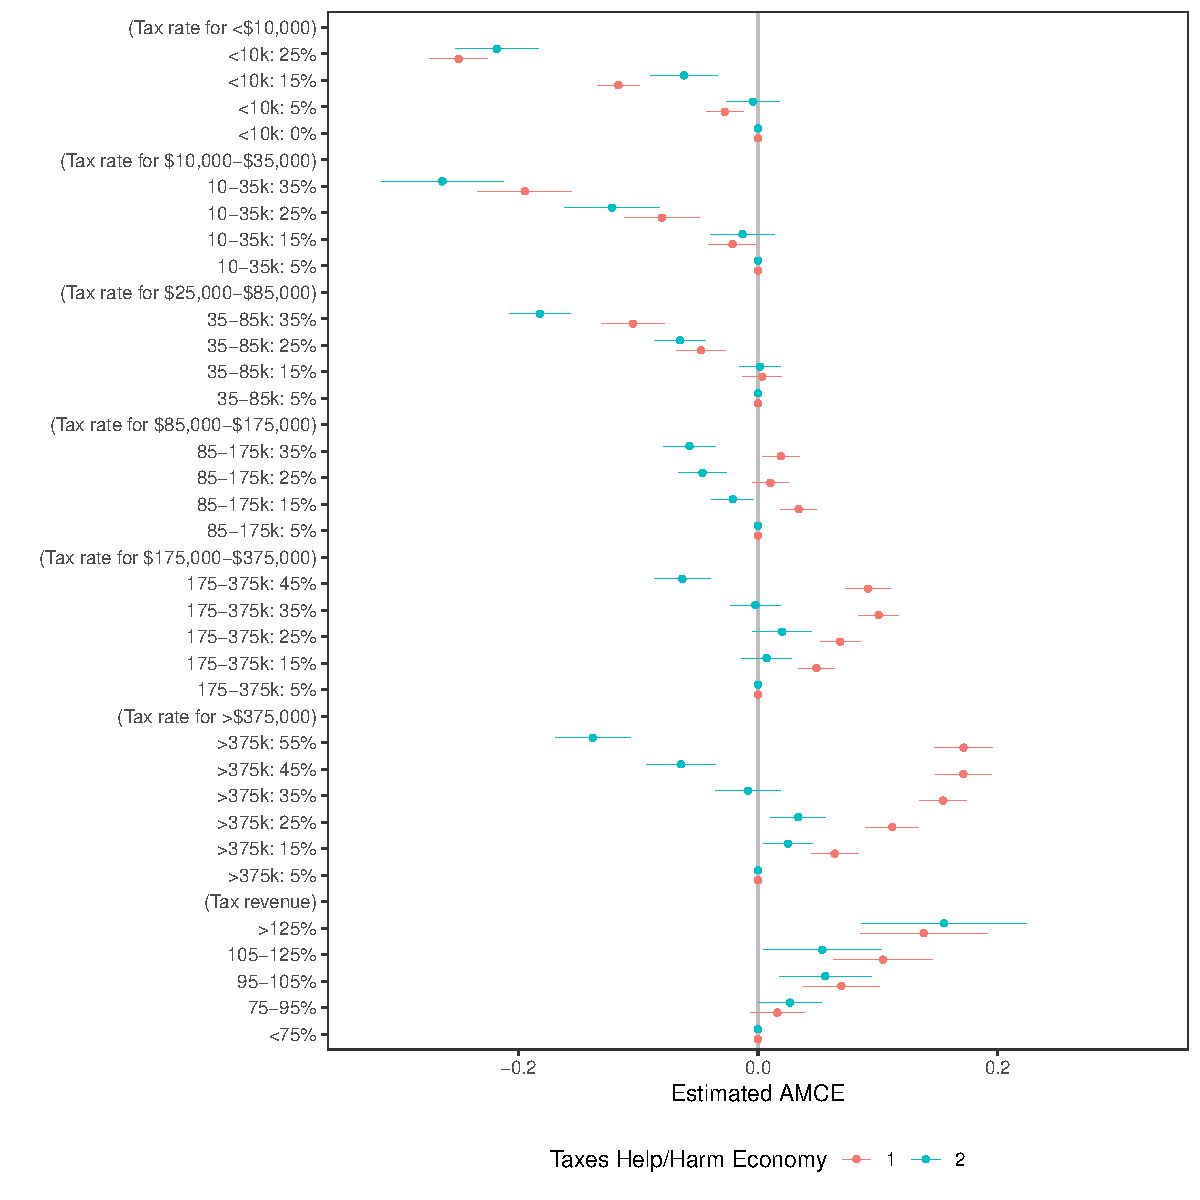
\includegraphics[width=\maxwidth]{figure/bms_subgroup_amce_appendix1-1} 

\end{knitrout}

\clearpage

\subsection{Subgroup Analysis for Ballard-Rosa et al. (2016), by ``Taxes Harm Economy'' Split using MMs}

\begin{knitrout}
\definecolor{shadecolor}{rgb}{0.969, 0.969, 0.969}\color{fgcolor}
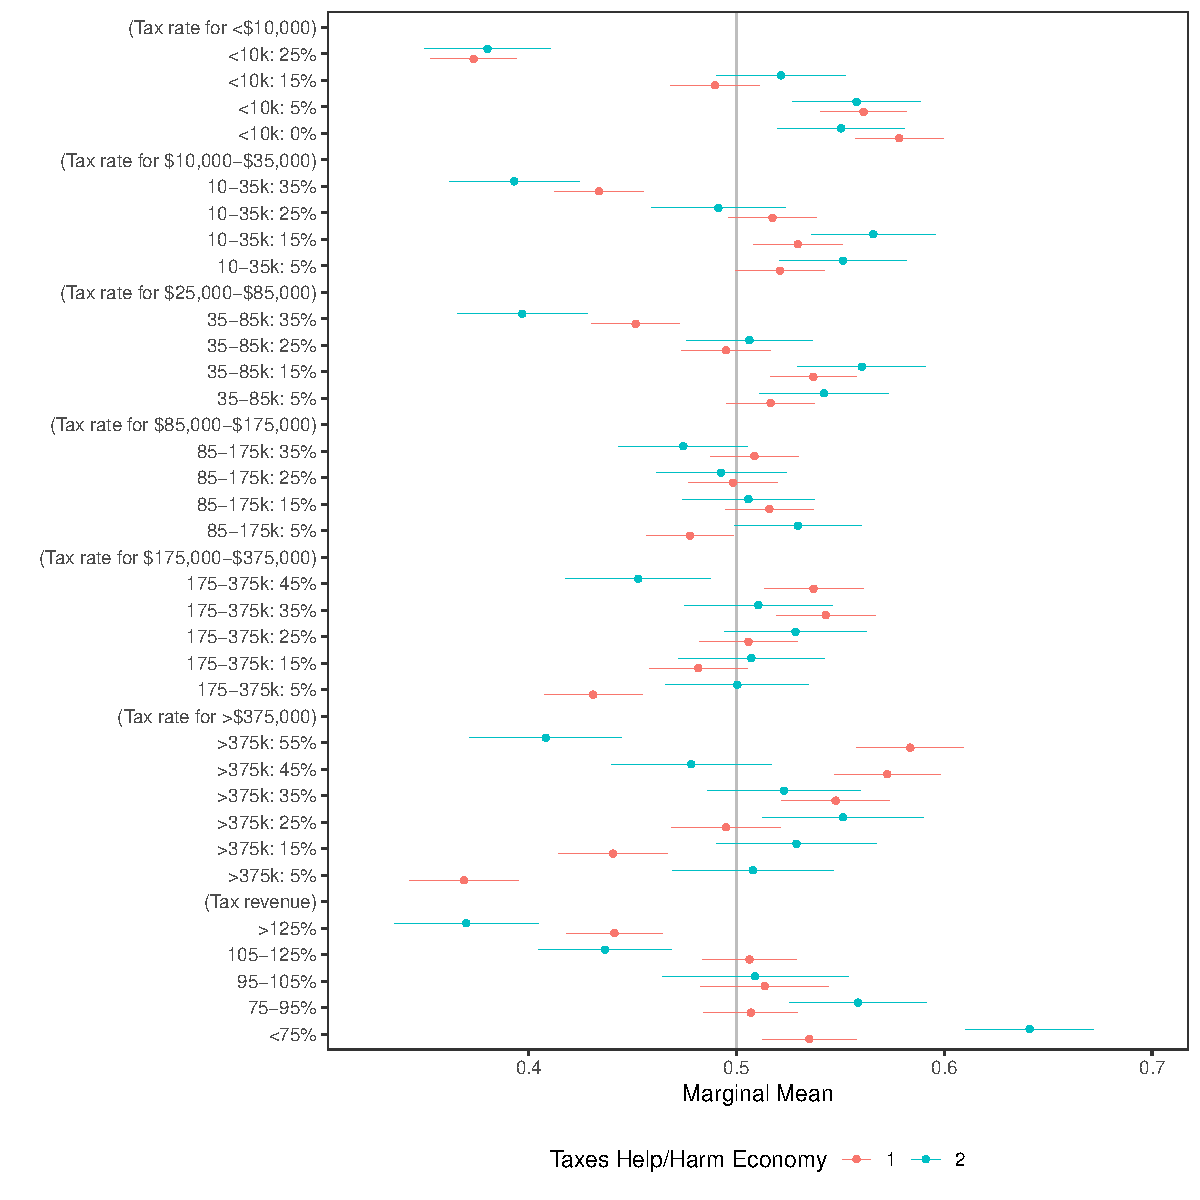
\includegraphics[width=\maxwidth]{figure/bms_subgroup_mm_appendix1-1} 

\end{knitrout}

\clearpage

\subsection{Subgroup Analysis for Ballard-Rosa et al. (2016), by Inequity Aversion using AMCEs}

\begin{knitrout}
\definecolor{shadecolor}{rgb}{0.969, 0.969, 0.969}\color{fgcolor}
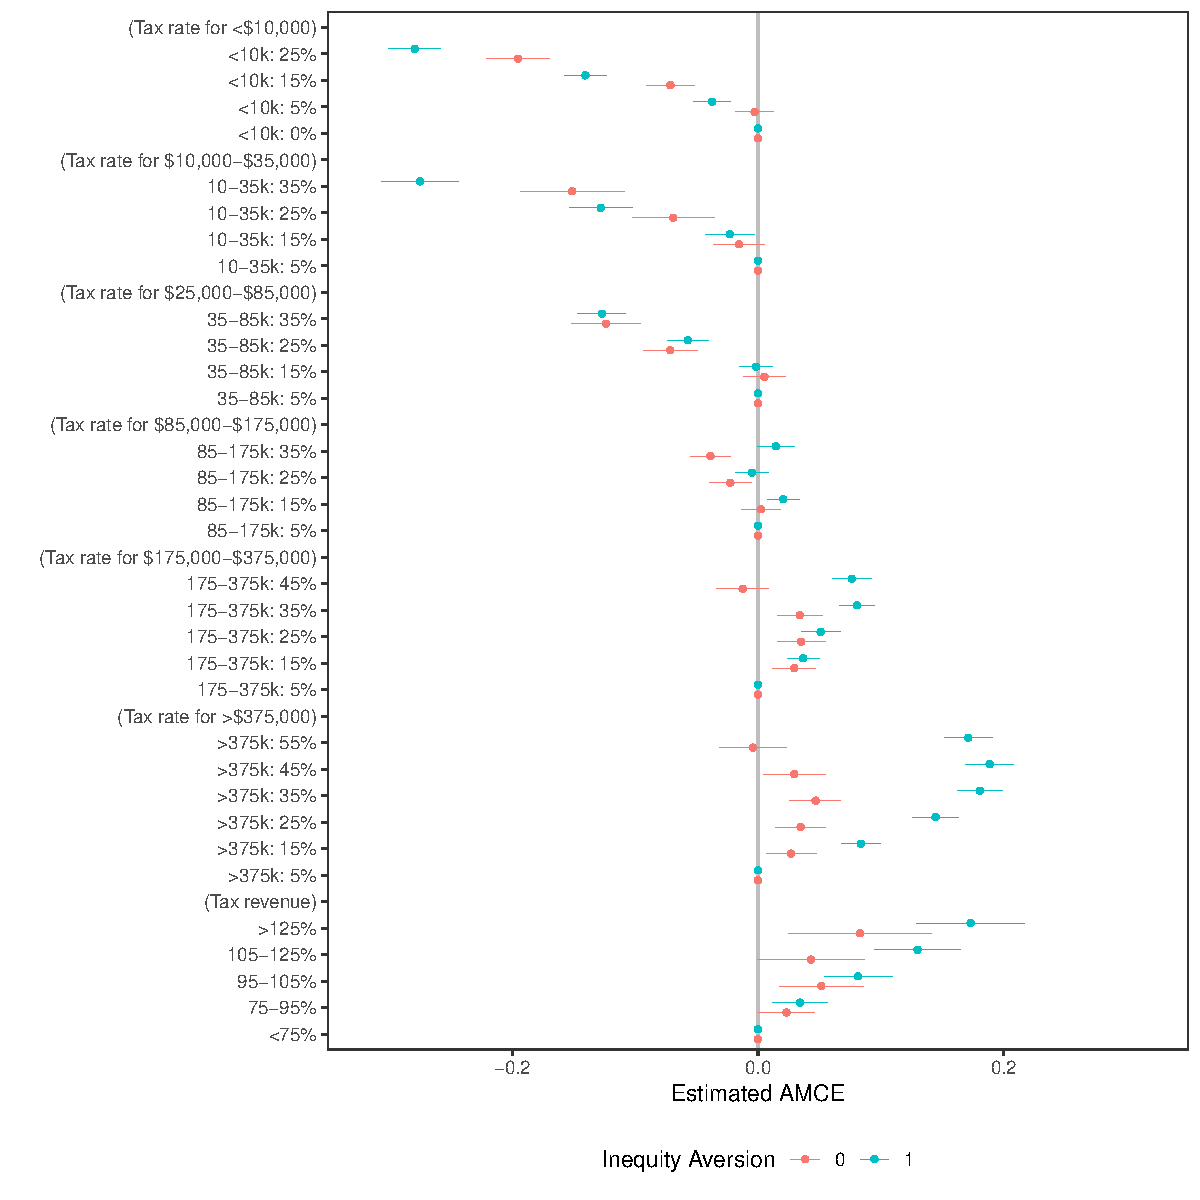
\includegraphics[width=\maxwidth]{figure/bms_subgroup_amce_appendix2-1} 

\end{knitrout}

\clearpage

\subsection{Subgroup Analysis for Ballard-Rosa et al. (2016), by Inequity Aversion using MMs}

\begin{knitrout}
\definecolor{shadecolor}{rgb}{0.969, 0.969, 0.969}\color{fgcolor}
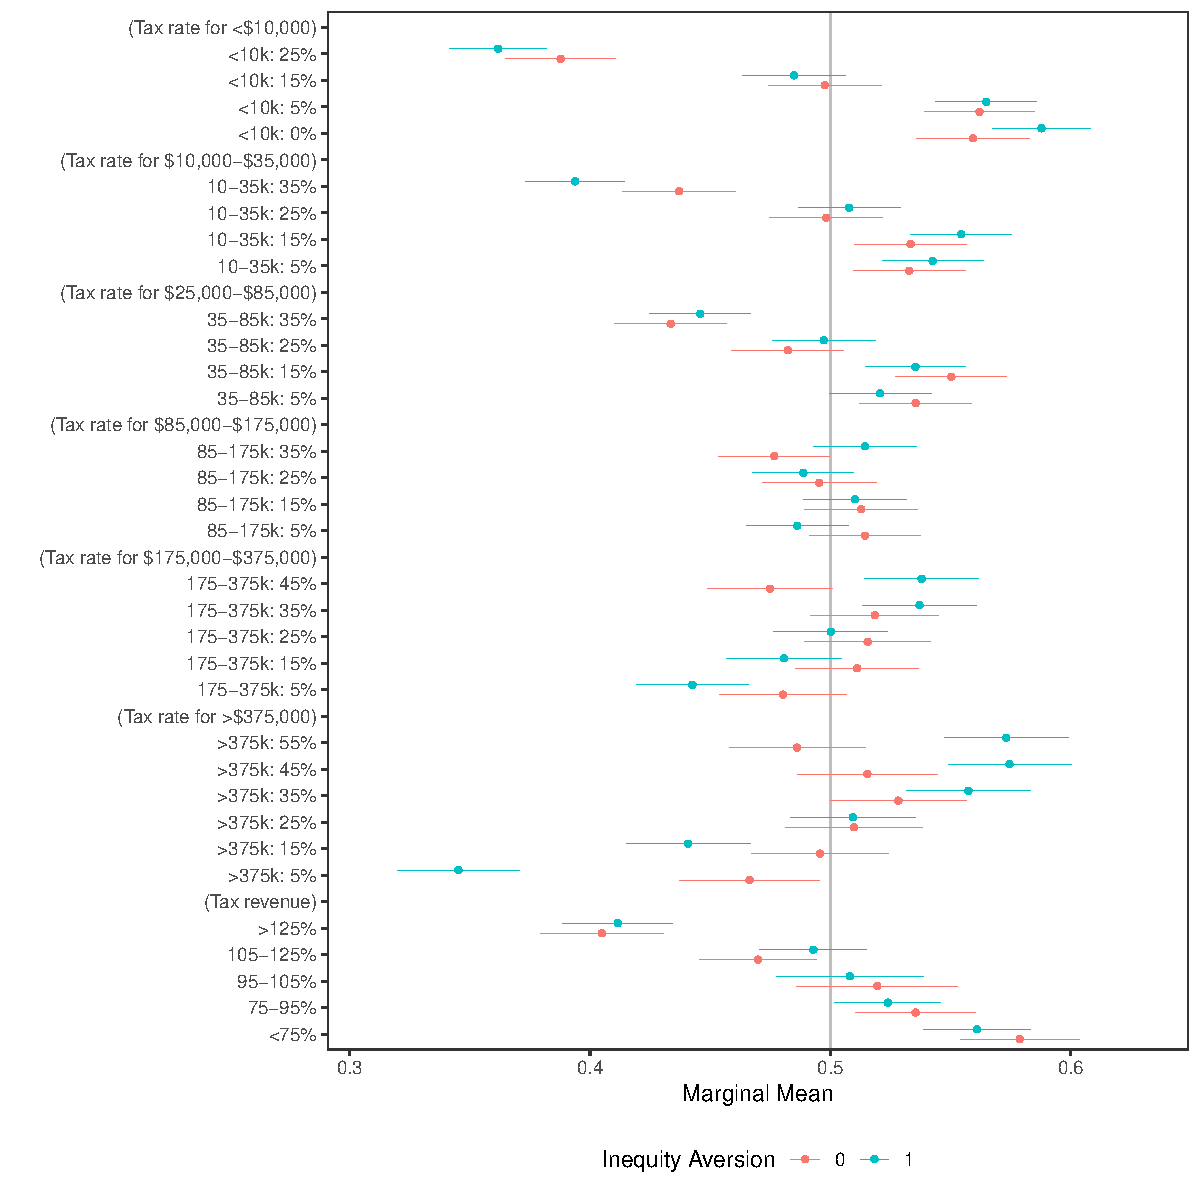
\includegraphics[width=\maxwidth]{figure/bms_subgroup_mm_appendix2-1} 

\end{knitrout}

\clearpage

\subsection{Comparison of Alternative Reference Categories for Ballard-Rosa et al. (2016) Tax Preference Experiment, by ``Taxes Harm Economy'' Split}



\begin{knitrout}
\definecolor{shadecolor}{rgb}{0.969, 0.969, 0.969}\color{fgcolor}
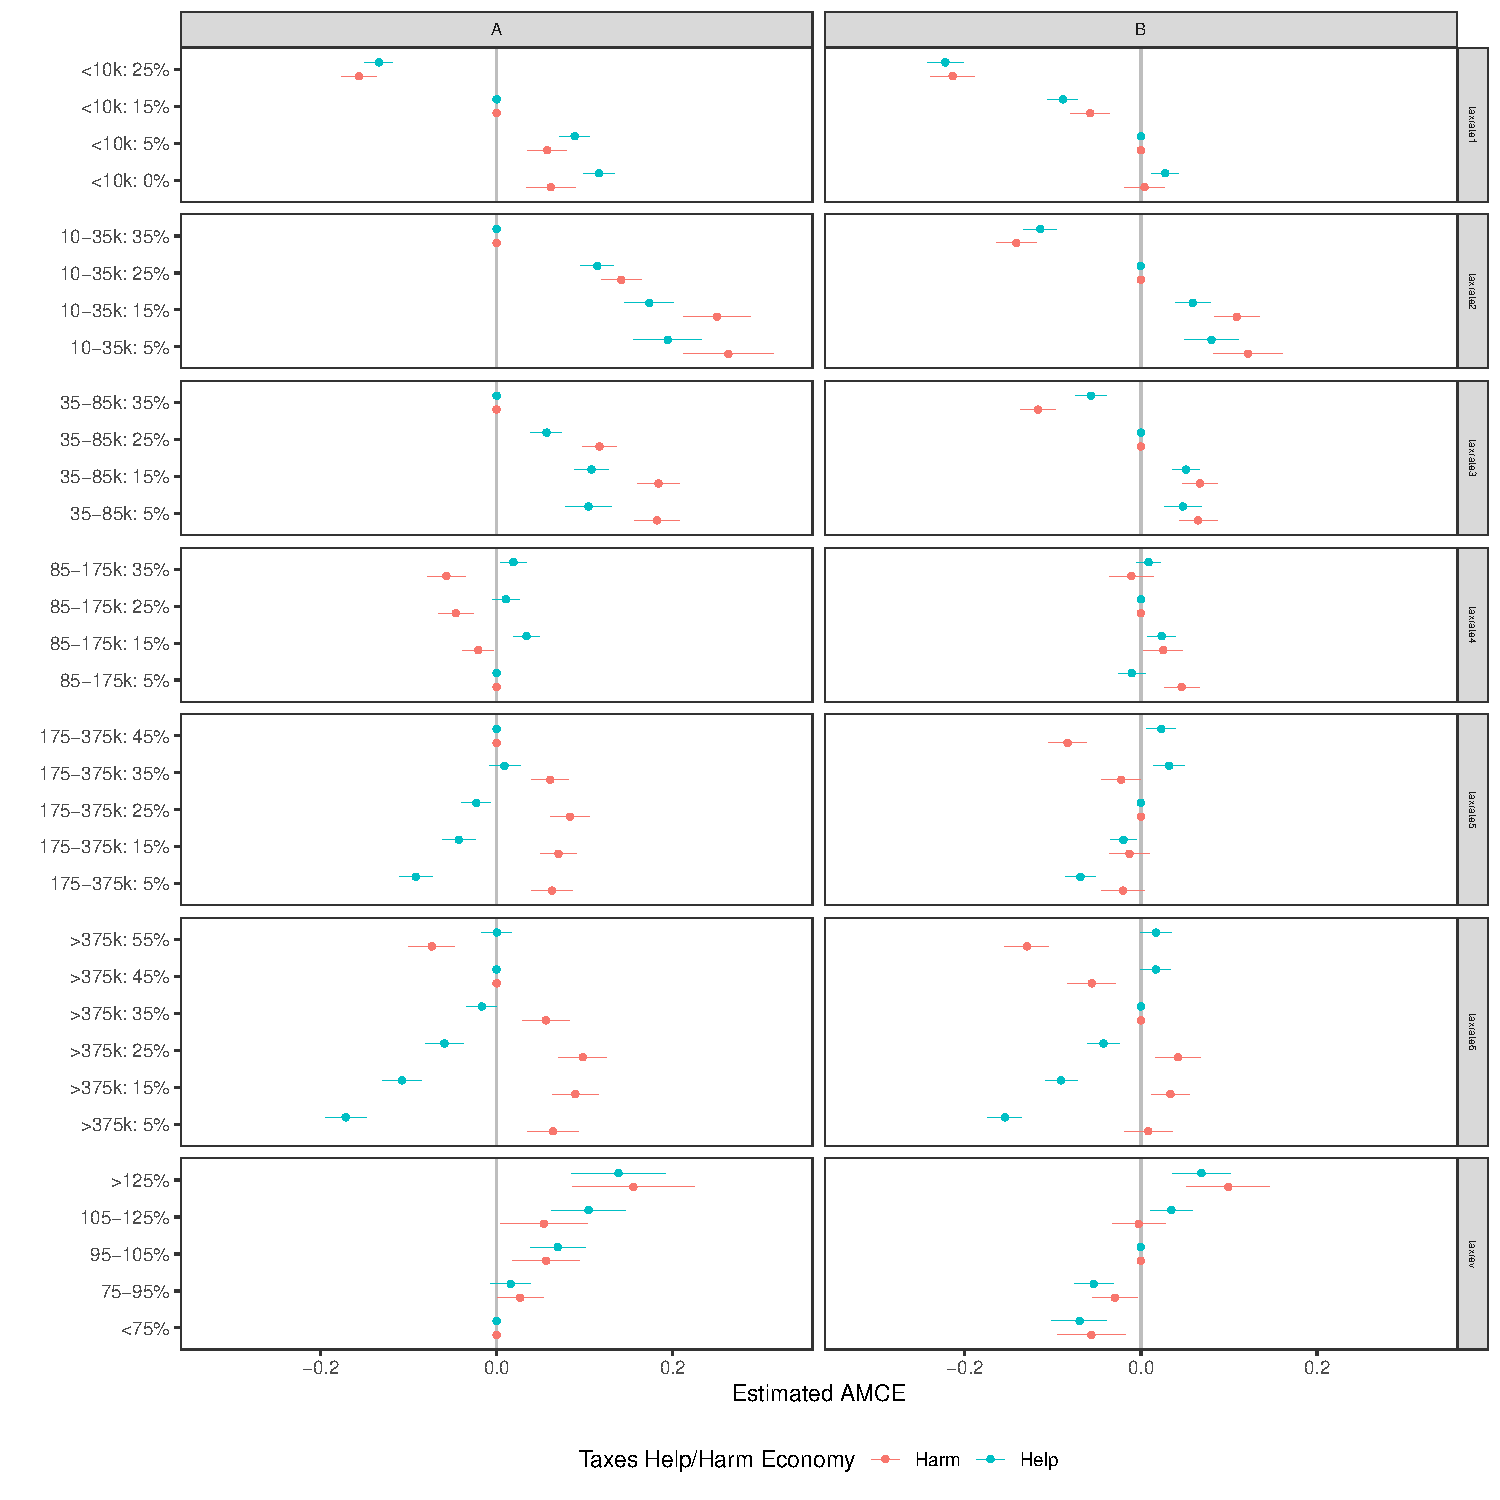
\includegraphics[width=\maxwidth]{figure/bms_subgroup_example_plot1-1} 

\end{knitrout}

\clearpage

\subsection{Comparison of Alternative Reference Categories for Ballard-Rosa et al. (2016) Tax Preference Experiment, by Inequity Aversion}



\begin{knitrout}
\definecolor{shadecolor}{rgb}{0.969, 0.969, 0.969}\color{fgcolor}
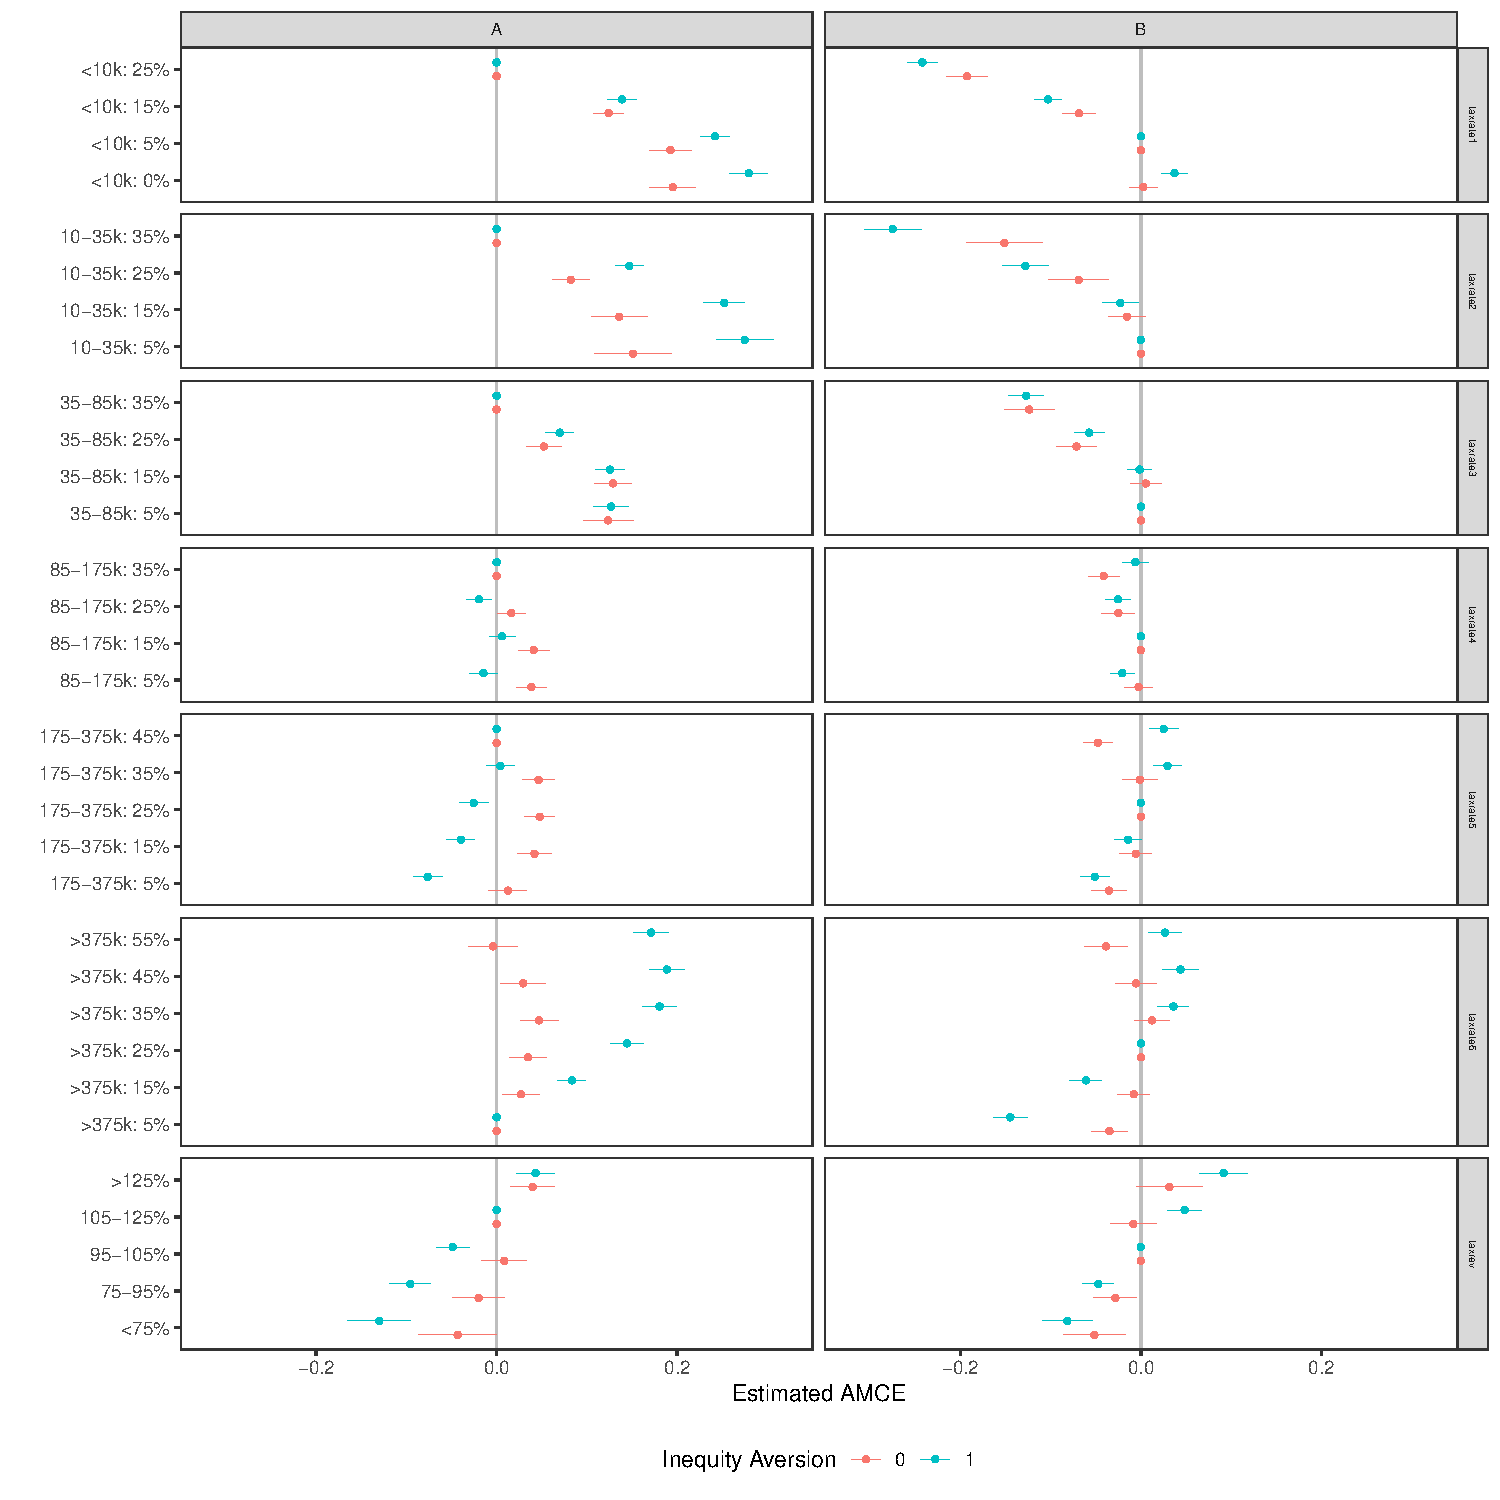
\includegraphics[width=\maxwidth]{figure/bms_subgroup_example_plot2-1} 

\end{knitrout}

\clearpage



\section{Bechtel and Scheve (2013) Climate Agreement Experiment}

\begin{knitrout}
\definecolor{shadecolor}{rgb}{0.969, 0.969, 0.969}\color{fgcolor}\begin{kframe}
\begin{verbatim}
##      outcome statistic                                 feature
## 1  choice_cj      amce    Costs to average household per month
## 2  choice_cj      amce    Costs to average household per month
## 3  choice_cj      amce    Costs to average household per month
## 4  choice_cj      amce    Costs to average household per month
## 5  choice_cj      amce    Costs to average household per month
## 6  choice_cj      amce                   Distribution of costs
## 7  choice_cj      amce                   Distribution of costs
## 8  choice_cj      amce                   Distribution of costs
## 9  choice_cj      amce                   Distribution of costs
## 10 choice_cj      amce       Number of participating countries
## 11 choice_cj      amce       Number of participating countries
## 12 choice_cj      amce       Number of participating countries
## 13 choice_cj      amce   Share of global emissions represented
## 14 choice_cj      amce   Share of global emissions represented
## 15 choice_cj      amce   Share of global emissions represented
## 16 choice_cj      amce Sanctions for missing reduction targets
## 17 choice_cj      amce Sanctions for missing reduction targets
## 18 choice_cj      amce Sanctions for missing reduction targets
## 19 choice_cj      amce Sanctions for missing reduction targets
## 20 choice_cj      amce                           Monitoring by
## 21 choice_cj      amce                           Monitoring by
## 22 choice_cj      amce                           Monitoring by
## 23 choice_cj      amce                           Monitoring by
##                                level     estimate   std.error           z
## 1                      \20028 per month  0.000000000          NA          NA
## 2                      \20056 per month -0.097845284 0.001402351  -69.772319
## 3                      \20084 per month -0.170008434 0.001468627 -115.760108
## 4                     \200113 per month -0.263769273 0.001471840 -179.210616
## 5                     \200141 per month -0.332856845 0.001422455 -234.001744
## 6                          Only rich  0.000000000          NA          NA
## 7         Prop. to current emissions  0.065924582 0.001340698   49.171839
## 8      Prop. to history of emissions  0.052479783 0.001345106   39.015350
## 9  Rich pay more than poor countries  0.057280714 0.001327647   43.144545
## 10                         20 of 192  0.000000000          NA          NA
## 11                         80 of 192  0.092728950 0.001141542   81.231296
## 12                        160 of 192  0.156435103 0.001175080  133.127175
## 13          40% of current emissions  0.000000000          NA          NA
## 14          60% of current emissions  0.022498908 0.001117762   20.128532
## 15          80% of current emissions  0.045174103 0.001125637   40.132047
## 16                              None  0.000000000          NA          NA
## 17               \2006 per hh and month  0.028464249 0.001308130   21.759490
## 18              \20017 per hh and month -0.018533001 0.001326110  -13.975465
## 19              \20023 per hh and month -0.053180963 0.001312140  -40.529947
## 20                   Your government  0.000000000          NA          NA
## 21                 Indep. commission  0.061714854 0.001323261   46.638460
## 22                    United Nations  0.024280174 0.001356516   17.898921
## 23                        Greenpeace -0.006573634 0.001377372   -4.772591
##                p        lower        upper
## 1             NA           NA           NA
## 2   0.000000e+00 -0.100593842 -0.095096727
## 3   0.000000e+00 -0.172886890 -0.167129978
## 4   0.000000e+00 -0.266654026 -0.260884521
## 5   0.000000e+00 -0.335644805 -0.330068886
## 6             NA           NA           NA
## 7   0.000000e+00  0.063296862  0.068552302
## 8   0.000000e+00  0.049843423  0.055116142
## 9   0.000000e+00  0.054678574  0.059882854
## 10            NA           NA           NA
## 11  0.000000e+00  0.090491569  0.094966332
## 12  0.000000e+00  0.154131988  0.158738218
## 13            NA           NA           NA
## 14  4.151128e-90  0.020308135  0.024689682
## 15  0.000000e+00  0.042967896  0.047380310
## 16            NA           NA           NA
## 17 5.616961e-105  0.025900360  0.031028137
## 18  2.200727e-44 -0.021132129 -0.015933874
## 19  0.000000e+00 -0.055752710 -0.050609216
## 20            NA           NA           NA
## 21  0.000000e+00  0.059121310  0.064308398
## 22  1.202281e-71  0.021621451  0.026938896
## 23  1.818711e-06 -0.009273234 -0.003874034
\end{verbatim}
\end{kframe}
\end{knitrout}


\begin{knitrout}
\definecolor{shadecolor}{rgb}{0.969, 0.969, 0.969}\color{fgcolor}\begin{kframe}
\begin{verbatim}
##      outcome statistic                                 feature
## 1  choice_cj        mm    Costs to average household per month
## 2  choice_cj        mm    Costs to average household per month
## 3  choice_cj        mm    Costs to average household per month
## 4  choice_cj        mm    Costs to average household per month
## 5  choice_cj        mm    Costs to average household per month
## 6  choice_cj        mm                   Distribution of costs
## 7  choice_cj        mm                   Distribution of costs
## 8  choice_cj        mm                   Distribution of costs
## 9  choice_cj        mm                   Distribution of costs
## 10 choice_cj        mm       Number of participating countries
## 11 choice_cj        mm       Number of participating countries
## 12 choice_cj        mm       Number of participating countries
## 13 choice_cj        mm   Share of global emissions represented
## 14 choice_cj        mm   Share of global emissions represented
## 15 choice_cj        mm   Share of global emissions represented
## 16 choice_cj        mm Sanctions for missing reduction targets
## 17 choice_cj        mm Sanctions for missing reduction targets
## 18 choice_cj        mm Sanctions for missing reduction targets
## 19 choice_cj        mm Sanctions for missing reduction targets
## 20 choice_cj        mm                           Monitoring by
## 21 choice_cj        mm                           Monitoring by
## 22 choice_cj        mm                           Monitoring by
## 23 choice_cj        mm                           Monitoring by
##                                level  estimate   std.error         z p
## 1                      \20028 per month 0.6729737 0.004126308 163.09342 0
## 2                      \20056 per month 0.5753704 0.004309124 133.52375 0
## 3                      \20084 per month 0.5028766 0.004395792 114.39955 0
## 4                     \200113 per month 0.4085284 0.004325220  94.45264 0
## 5                     \200141 per month 0.3394765 0.004148381  81.83349 0
## 6                          Only rich 0.4570055 0.003911228 116.84452 0
## 7         Prop. to current emissions 0.5216566 0.003926015 132.87176 0
## 8      Prop. to history of emissions 0.5087938 0.003917689 129.87090 0
## 9  Rich pay more than poor countries 0.5127165 0.003924942 130.63032 0
## 10                         20 of 192 0.4182276 0.003341616 125.15729 0
## 11                         80 of 192 0.5089863 0.003399306 149.73245 0
## 12                        160 of 192 0.5737857 0.003373566 170.08288 0
## 13          40% of current emissions 0.4781113 0.003380328 141.43933 0
## 14          60% of current emissions 0.4999291 0.003407780 146.70227 0
## 15          80% of current emissions 0.5222143 0.003402419 153.48325 0
## 16                              None 0.5106586 0.003932951 129.84109 0
## 17               \2006 per hh and month 0.5412417 0.003913371 138.30573 0
## 18              \20017 per hh and month 0.4928567 0.003908225 126.10754 0
## 19              \20023 per hh and month 0.4552868 0.003914718 116.30129 0
## 20                   Your government 0.4813399 0.003912654 123.02130 0
## 21                 Indep. commission 0.5426752 0.003901770 139.08437 0
## 22                    United Nations 0.5032115 0.003941043 127.68486 0
## 23                        Greenpeace 0.4725424 0.003920333 120.53630 0
##        lower     upper
## 1  0.6648863 0.6810611
## 2  0.5669247 0.5838161
## 3  0.4942610 0.5114922
## 4  0.4000512 0.4170057
## 5  0.3313459 0.3476072
## 6  0.4493397 0.4646714
## 7  0.5139617 0.5293514
## 8  0.5011153 0.5164723
## 9  0.5050237 0.5204092
## 10 0.4116781 0.4247770
## 11 0.5023238 0.5156488
## 12 0.5671737 0.5803978
## 13 0.4714860 0.4847366
## 14 0.4932500 0.5066083
## 15 0.5155456 0.5288829
## 16 0.5029502 0.5183671
## 17 0.5335716 0.5489118
## 18 0.4851967 0.5005167
## 19 0.4476140 0.4629595
## 20 0.4736712 0.4890085
## 21 0.5350279 0.5503225
## 22 0.4954872 0.5109358
## 23 0.4648587 0.4802262
\end{verbatim}
\end{kframe}
\end{knitrout}

\begin{knitrout}
\definecolor{shadecolor}{rgb}{0.969, 0.969, 0.969}\color{fgcolor}
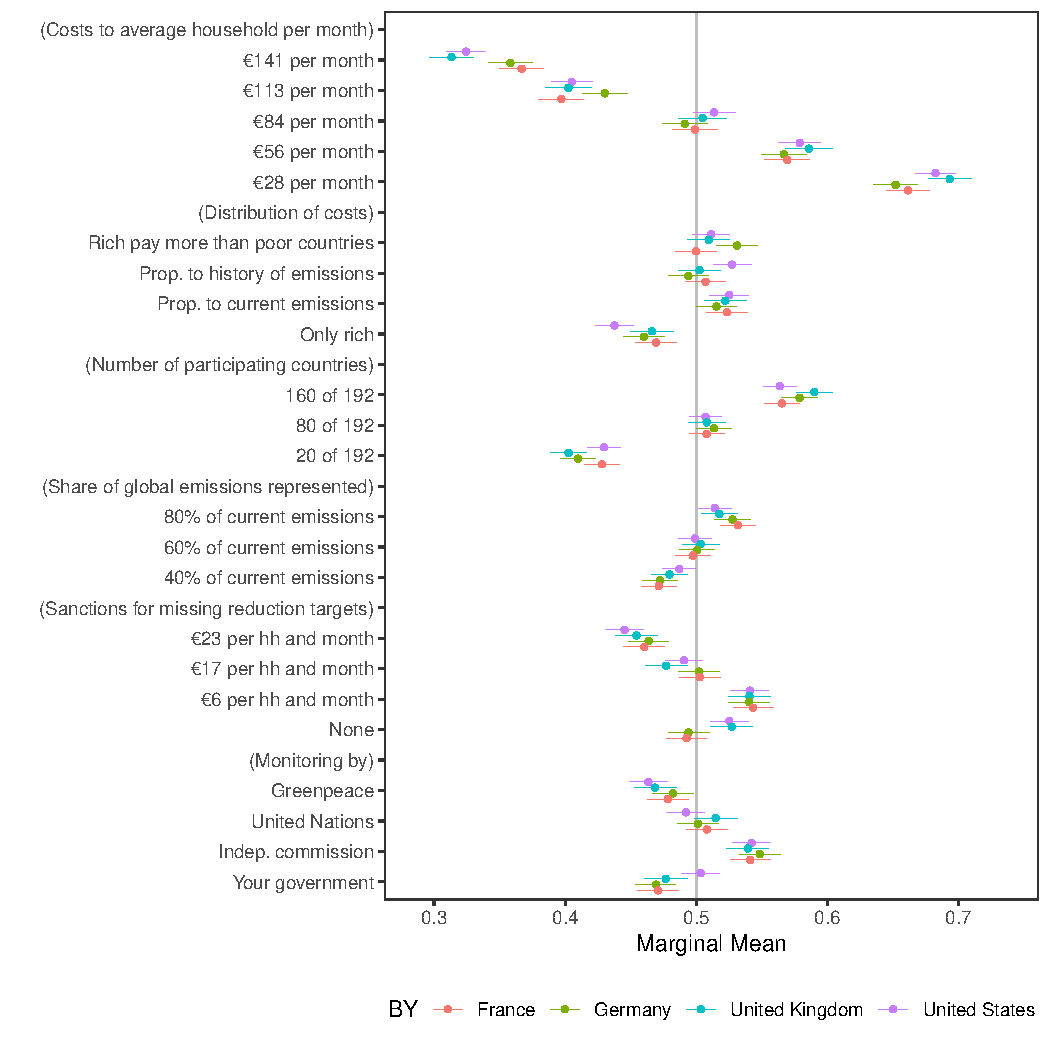
\includegraphics[width=\maxwidth]{figure/bechtel_subgroup_mm-1} 
\begin{kframe}\begin{verbatim}
##                BY   outcome statistic
## 1          France choice_cj        mm
## 2          France choice_cj        mm
## 3          France choice_cj        mm
## 4          France choice_cj        mm
## 5          France choice_cj        mm
## 6          France choice_cj        mm
## 7          France choice_cj        mm
## 8          France choice_cj        mm
## 9          France choice_cj        mm
## 10         France choice_cj        mm
## 11         France choice_cj        mm
## 12         France choice_cj        mm
## 13         France choice_cj        mm
## 14         France choice_cj        mm
## 15         France choice_cj        mm
## 16         France choice_cj        mm
## 17         France choice_cj        mm
## 18         France choice_cj        mm
## 19         France choice_cj        mm
## 20         France choice_cj        mm
## 21         France choice_cj        mm
## 22         France choice_cj        mm
## 23         France choice_cj        mm
## 24        Germany choice_cj        mm
## 25        Germany choice_cj        mm
## 26        Germany choice_cj        mm
## 27        Germany choice_cj        mm
## 28        Germany choice_cj        mm
## 29        Germany choice_cj        mm
## 30        Germany choice_cj        mm
## 31        Germany choice_cj        mm
## 32        Germany choice_cj        mm
## 33        Germany choice_cj        mm
## 34        Germany choice_cj        mm
## 35        Germany choice_cj        mm
## 36        Germany choice_cj        mm
## 37        Germany choice_cj        mm
## 38        Germany choice_cj        mm
## 39        Germany choice_cj        mm
## 40        Germany choice_cj        mm
## 41        Germany choice_cj        mm
## 42        Germany choice_cj        mm
## 43        Germany choice_cj        mm
## 44        Germany choice_cj        mm
## 45        Germany choice_cj        mm
## 46        Germany choice_cj        mm
## 47 United Kingdom choice_cj        mm
## 48 United Kingdom choice_cj        mm
## 49 United Kingdom choice_cj        mm
## 50 United Kingdom choice_cj        mm
## 51 United Kingdom choice_cj        mm
## 52 United Kingdom choice_cj        mm
## 53 United Kingdom choice_cj        mm
## 54 United Kingdom choice_cj        mm
## 55 United Kingdom choice_cj        mm
## 56 United Kingdom choice_cj        mm
## 57 United Kingdom choice_cj        mm
## 58 United Kingdom choice_cj        mm
## 59 United Kingdom choice_cj        mm
## 60 United Kingdom choice_cj        mm
## 61 United Kingdom choice_cj        mm
## 62 United Kingdom choice_cj        mm
## 63 United Kingdom choice_cj        mm
## 64 United Kingdom choice_cj        mm
## 65 United Kingdom choice_cj        mm
## 66 United Kingdom choice_cj        mm
## 67 United Kingdom choice_cj        mm
## 68 United Kingdom choice_cj        mm
## 69 United Kingdom choice_cj        mm
## 70  United States choice_cj        mm
## 71  United States choice_cj        mm
## 72  United States choice_cj        mm
## 73  United States choice_cj        mm
## 74  United States choice_cj        mm
## 75  United States choice_cj        mm
## 76  United States choice_cj        mm
## 77  United States choice_cj        mm
## 78  United States choice_cj        mm
## 79  United States choice_cj        mm
## 80  United States choice_cj        mm
## 81  United States choice_cj        mm
## 82  United States choice_cj        mm
## 83  United States choice_cj        mm
## 84  United States choice_cj        mm
## 85  United States choice_cj        mm
## 86  United States choice_cj        mm
## 87  United States choice_cj        mm
## 88  United States choice_cj        mm
## 89  United States choice_cj        mm
## 90  United States choice_cj        mm
## 91  United States choice_cj        mm
## 92  United States choice_cj        mm
##                                    feature
## 1     Costs to average household per month
## 2     Costs to average household per month
## 3     Costs to average household per month
## 4     Costs to average household per month
## 5     Costs to average household per month
## 6                    Distribution of costs
## 7                    Distribution of costs
## 8                    Distribution of costs
## 9                    Distribution of costs
## 10       Number of participating countries
## 11       Number of participating countries
## 12       Number of participating countries
## 13   Share of global emissions represented
## 14   Share of global emissions represented
## 15   Share of global emissions represented
## 16 Sanctions for missing reduction targets
## 17 Sanctions for missing reduction targets
## 18 Sanctions for missing reduction targets
## 19 Sanctions for missing reduction targets
## 20                           Monitoring by
## 21                           Monitoring by
## 22                           Monitoring by
## 23                           Monitoring by
## 24    Costs to average household per month
## 25    Costs to average household per month
## 26    Costs to average household per month
## 27    Costs to average household per month
## 28    Costs to average household per month
## 29                   Distribution of costs
## 30                   Distribution of costs
## 31                   Distribution of costs
## 32                   Distribution of costs
## 33       Number of participating countries
## 34       Number of participating countries
## 35       Number of participating countries
## 36   Share of global emissions represented
## 37   Share of global emissions represented
## 38   Share of global emissions represented
## 39 Sanctions for missing reduction targets
## 40 Sanctions for missing reduction targets
## 41 Sanctions for missing reduction targets
## 42 Sanctions for missing reduction targets
## 43                           Monitoring by
## 44                           Monitoring by
## 45                           Monitoring by
## 46                           Monitoring by
## 47    Costs to average household per month
## 48    Costs to average household per month
## 49    Costs to average household per month
## 50    Costs to average household per month
## 51    Costs to average household per month
## 52                   Distribution of costs
## 53                   Distribution of costs
## 54                   Distribution of costs
## 55                   Distribution of costs
## 56       Number of participating countries
## 57       Number of participating countries
## 58       Number of participating countries
## 59   Share of global emissions represented
## 60   Share of global emissions represented
## 61   Share of global emissions represented
## 62 Sanctions for missing reduction targets
## 63 Sanctions for missing reduction targets
## 64 Sanctions for missing reduction targets
## 65 Sanctions for missing reduction targets
## 66                           Monitoring by
## 67                           Monitoring by
## 68                           Monitoring by
## 69                           Monitoring by
## 70    Costs to average household per month
## 71    Costs to average household per month
## 72    Costs to average household per month
## 73    Costs to average household per month
## 74    Costs to average household per month
## 75                   Distribution of costs
## 76                   Distribution of costs
## 77                   Distribution of costs
## 78                   Distribution of costs
## 79       Number of participating countries
## 80       Number of participating countries
## 81       Number of participating countries
## 82   Share of global emissions represented
## 83   Share of global emissions represented
## 84   Share of global emissions represented
## 85 Sanctions for missing reduction targets
## 86 Sanctions for missing reduction targets
## 87 Sanctions for missing reduction targets
## 88 Sanctions for missing reduction targets
## 89                           Monitoring by
## 90                           Monitoring by
## 91                           Monitoring by
## 92                           Monitoring by
##                                level  estimate   std.error        z
## 1                      \20028 per month 0.6613316 0.008322408 79.46397
## 2                      \20056 per month 0.5693159 0.008660576 65.73649
## 3                      \20084 per month 0.4989851 0.008884067 56.16629
## 4                     \200113 per month 0.3970867 0.008722819 45.52275
## 5                     \200141 per month 0.3667680 0.008567482 42.80931
## 6                          Only rich 0.4694590 0.007936306 59.15334
## 7         Prop. to current emissions 0.5234480 0.007931229 65.99834
## 8      Prop. to history of emissions 0.5070668 0.007869017 64.43840
## 9  Rich pay more than poor countries 0.4998164 0.007880458 63.42479
## 10                         20 of 192 0.4280902 0.006737716 63.53639
## 11                         80 of 192 0.5079278 0.006874025 73.89089
## 12                        160 of 192 0.5652797 0.006810168 83.00524
## 13          40% of current emissions 0.4714751 0.006806164 69.27178
## 14          60% of current emissions 0.4972686 0.006865214 72.43307
## 15          80% of current emissions 0.5316843 0.006854741 77.56447
## 16                              None 0.4925810 0.007922009 62.17879
## 17               \2006 per hh and month 0.5433092 0.007813932 69.53084
## 18              \20017 per hh and month 0.5026263 0.007925773 63.41668
## 19              \20023 per hh and month 0.4603338 0.007923589 58.09663
## 20                   Your government 0.4707127 0.007932301 59.34126
## 21                 Indep. commission 0.5410998 0.007756003 69.76529
## 22                    United Nations 0.5079832 0.007952899 63.87396
## 23                        Greenpeace 0.4783606 0.007954893 60.13414
## 24                     \20028 per month 0.6520203 0.008538989 76.35801
## 25                     \20056 per month 0.5667114 0.008678489 65.30070
## 26                     \20084 per month 0.4912437 0.008871631 55.37242
## 27                    \200113 per month 0.4301405 0.008828618 48.72116
## 28                    \200141 per month 0.3582373 0.008565178 41.82486
## 29                         Only rich 0.4600371 0.007930387 58.00941
## 30        Prop. to current emissions 0.5153914 0.007901516 65.22689
## 31     Prop. to history of emissions 0.4940093 0.007884299 62.65736
## 32 Rich pay more than poor countries 0.5312310 0.008045629 66.02727
## 33                         20 of 192 0.4098216 0.006744866 60.76052
## 34                         80 of 192 0.5134710 0.006855305 74.90126
## 35                        160 of 192 0.5787895 0.006863767 84.32534
## 36          40% of current emissions 0.4723114 0.006837992 69.07165
## 37          60% of current emissions 0.5007192 0.006884860 72.72757
## 38          80% of current emissions 0.5275701 0.006914689 76.29700
## 39                              None 0.4940875 0.007989972 61.83845
## 40               \2006 per hh and month 0.5402615 0.007912846 68.27651
## 41              \20017 per hh and month 0.5021986 0.007968977 63.01920
## 42              \20023 per hh and month 0.4636031 0.007886215 58.78651
## 43                   Your government 0.4691111 0.007850099 59.75862
## 44                 Indep. commission 0.5483852 0.007959662 68.89553
## 45                    United Nations 0.5011726 0.007951130 63.03162
## 46                        Greenpeace 0.4823303 0.007989396 60.37131
## 47                     \20028 per month 0.6934878 0.008424386 82.31909
## 48                     \20056 per month 0.5859726 0.009034648 64.85838
## 49                     \20084 per month 0.5048116 0.009338115 54.05926
## 50                    \200113 per month 0.4024743 0.008986324 44.78743
## 51                    \200141 per month 0.3132586 0.008508073 36.81898
## 52                         Only rich 0.4661502 0.008199944 56.84798
## 53        Prop. to current emissions 0.5221721 0.008206555 63.62865
## 54     Prop. to history of emissions 0.5024308 0.008263298 60.80270
## 55 Rich pay more than poor countries 0.5095266 0.008245511 61.79443
## 56                         20 of 192 0.4025534 0.006980412 57.66899
## 57                         80 of 192 0.5079030 0.007155688 70.97892
## 58                        160 of 192 0.5899041 0.007002721 84.23928
## 59          40% of current emissions 0.4795459 0.007060046 67.92391
## 60          60% of current emissions 0.5032446 0.007215347 69.74642
## 61          80% of current emissions 0.5176103 0.007113186 72.76772
## 62                              None 0.5270756 0.008192395 64.33718
## 63               \2006 per hh and month 0.5405720 0.008214268 65.80890
## 64              \20017 per hh and month 0.4769717 0.008165885 58.41029
## 65              \20023 per hh and month 0.4544697 0.008288953 54.82836
## 66                   Your government 0.4768185 0.008212548 58.05975
## 67                 Indep. commission 0.5392912 0.008128128 66.34876
## 68                    United Nations 0.5147711 0.008330945 61.79024
## 69                        Greenpeace 0.4686105 0.008208476 57.08861
## 70                     \20028 per month 0.6824518 0.007763555 87.90454
## 71                     \20056 per month 0.5789579 0.008147606 71.05866
## 72                     \20084 per month 0.5136585 0.008166584 62.89760
## 73                    \200113 per month 0.4051599 0.008111491 49.94888
## 74                    \200141 per month 0.3244207 0.007630904 42.51406
## 75                         Only rich 0.4375458 0.007282486 60.08192
## 76        Prop. to current emissions 0.5249692 0.007413118 70.81625
## 77     Prop. to history of emissions 0.5272909 0.007370877 71.53706
## 78 Rich pay more than poor countries 0.5112713 0.007298410 70.05243
## 79                         20 of 192 0.4296274 0.006300652 68.18777
## 80                         80 of 192 0.5070832 0.006363026 79.69215
## 81                        160 of 192 0.5636379 0.006344643 88.83682
## 82          40% of current emissions 0.4870124 0.006373185 76.41585
## 83          60% of current emissions 0.4988350 0.006362123 78.40701
## 84          80% of current emissions 0.5141367 0.006379806 80.58813
## 85                              None 0.5251766 0.007391775 71.04878
## 86               \2006 per hh and month 0.5408734 0.007408935 73.00285
## 87              \20017 per hh and month 0.4906273 0.007267688 67.50804
## 88              \20023 per hh and month 0.4452759 0.007296972 61.02201
## 89                   Your government 0.5033382 0.007350454 68.47716
## 90                 Indep. commission 0.5422171 0.007403558 73.23736
## 91                    United Nations 0.4920508 0.007361504 66.84108
## 92                        Greenpeace 0.4634591 0.007284021 63.62682
##                p     lower     upper        country
## 1   0.000000e+00 0.6450199 0.6776432         France
## 2   0.000000e+00 0.5523415 0.5862903         France
## 3   0.000000e+00 0.4815727 0.5163976         France
## 4   0.000000e+00 0.3799903 0.4141831         France
## 5   0.000000e+00 0.3499761 0.3835600         France
## 6   0.000000e+00 0.4539041 0.4850139         France
## 7   0.000000e+00 0.5079031 0.5389929         France
## 8   0.000000e+00 0.4916438 0.5224898         France
## 9   0.000000e+00 0.4843710 0.5152619         France
## 10  0.000000e+00 0.4148845 0.4412958         France
## 11  0.000000e+00 0.4944550 0.5214007         France
## 12  0.000000e+00 0.5519320 0.5786274         France
## 13  0.000000e+00 0.4581352 0.4848149         France
## 14  0.000000e+00 0.4838130 0.5107242         France
## 15  0.000000e+00 0.5182493 0.5451194         France
## 16  0.000000e+00 0.4770541 0.5081078         France
## 17  0.000000e+00 0.5279942 0.5586243         France
## 18  0.000000e+00 0.4870920 0.5181605         France
## 19  0.000000e+00 0.4448038 0.4758637         France
## 20  0.000000e+00 0.4551657 0.4862597         France
## 21  0.000000e+00 0.5258983 0.5563013         France
## 22  0.000000e+00 0.4923958 0.5235706         France
## 23  0.000000e+00 0.4627693 0.4939519         France
## 24  0.000000e+00 0.6352841 0.6687564        Germany
## 25  0.000000e+00 0.5497018 0.5837209        Germany
## 26  0.000000e+00 0.4738556 0.5086317        Germany
## 27  0.000000e+00 0.4128368 0.4474443        Germany
## 28  0.000000e+00 0.3414499 0.3750248        Germany
## 29  0.000000e+00 0.4444938 0.4755803        Germany
## 30  0.000000e+00 0.4999047 0.5308781        Germany
## 31  0.000000e+00 0.4785564 0.5094622        Germany
## 32  0.000000e+00 0.5154618 0.5470001        Germany
## 33  0.000000e+00 0.3966019 0.4230413        Germany
## 34  0.000000e+00 0.5000348 0.5269071        Germany
## 35  0.000000e+00 0.5653368 0.5922422        Germany
## 36  0.000000e+00 0.4589092 0.4857136        Germany
## 37  0.000000e+00 0.4872251 0.5142132        Germany
## 38  0.000000e+00 0.5140175 0.5411226        Germany
## 39  0.000000e+00 0.4784274 0.5097476        Germany
## 40  0.000000e+00 0.5247526 0.5557704        Germany
## 41  0.000000e+00 0.4865797 0.5178175        Germany
## 42  0.000000e+00 0.4481464 0.4790598        Germany
## 43  0.000000e+00 0.4537252 0.4844970        Germany
## 44  0.000000e+00 0.5327845 0.5639858        Germany
## 45  0.000000e+00 0.4855887 0.5167566        Germany
## 46  0.000000e+00 0.4666714 0.4979892        Germany
## 47  0.000000e+00 0.6769763 0.7099993 United Kingdom
## 48  0.000000e+00 0.5682650 0.6036802 United Kingdom
## 49  0.000000e+00 0.4865092 0.5231140 United Kingdom
## 50  0.000000e+00 0.3848615 0.4200872 United Kingdom
## 51 9.175209e-297 0.2965831 0.3299341 United Kingdom
## 52  0.000000e+00 0.4500786 0.4822218 United Kingdom
## 53  0.000000e+00 0.5060875 0.5382566 United Kingdom
## 54  0.000000e+00 0.4862350 0.5186266 United Kingdom
## 55  0.000000e+00 0.4933657 0.5256875 United Kingdom
## 56  0.000000e+00 0.3888720 0.4162347 United Kingdom
## 57  0.000000e+00 0.4938781 0.5219279 United Kingdom
## 58  0.000000e+00 0.5761791 0.6036292 United Kingdom
## 59  0.000000e+00 0.4657085 0.4933834 United Kingdom
## 60  0.000000e+00 0.4891028 0.5173864 United Kingdom
## 61  0.000000e+00 0.5036687 0.5315519 United Kingdom
## 62  0.000000e+00 0.5110188 0.5431324 United Kingdom
## 63  0.000000e+00 0.5244723 0.5566716 United Kingdom
## 64  0.000000e+00 0.4609668 0.4929765 United Kingdom
## 65  0.000000e+00 0.4382236 0.4707157 United Kingdom
## 66  0.000000e+00 0.4607222 0.4929148 United Kingdom
## 67  0.000000e+00 0.5233604 0.5552221 United Kingdom
## 68  0.000000e+00 0.4984427 0.5310994 United Kingdom
## 69  0.000000e+00 0.4525221 0.4846988 United Kingdom
## 70  0.000000e+00 0.6672355 0.6976681  United States
## 71  0.000000e+00 0.5629889 0.5949270  United States
## 72  0.000000e+00 0.4976523 0.5296647  United States
## 73  0.000000e+00 0.3892617 0.4210581  United States
## 74  0.000000e+00 0.3094644 0.3393770  United States
## 75  0.000000e+00 0.4232724 0.4518192  United States
## 76  0.000000e+00 0.5104398 0.5394987  United States
## 77  0.000000e+00 0.5128442 0.5417375  United States
## 78  0.000000e+00 0.4969667 0.5255759  United States
## 79  0.000000e+00 0.4172784 0.4419765  United States
## 80  0.000000e+00 0.4946119 0.5195545  United States
## 81  0.000000e+00 0.5512027 0.5760732  United States
## 82  0.000000e+00 0.4745211 0.4995036  United States
## 83  0.000000e+00 0.4863655 0.5113045  United States
## 84  0.000000e+00 0.5016325 0.5266409  United States
## 85  0.000000e+00 0.5106890 0.5396642  United States
## 86  0.000000e+00 0.5263521 0.5553946  United States
## 87  0.000000e+00 0.4763829 0.5048717  United States
## 88  0.000000e+00 0.4309741 0.4595777  United States
## 89  0.000000e+00 0.4889316 0.5177448  United States
## 90  0.000000e+00 0.5277064 0.5567278  United States
## 91  0.000000e+00 0.4776225 0.5064791  United States
## 92  0.000000e+00 0.4491827 0.4777355  United States
\end{verbatim}
\end{kframe}
\end{knitrout}

\begin{knitrout}
\definecolor{shadecolor}{rgb}{0.969, 0.969, 0.969}\color{fgcolor}
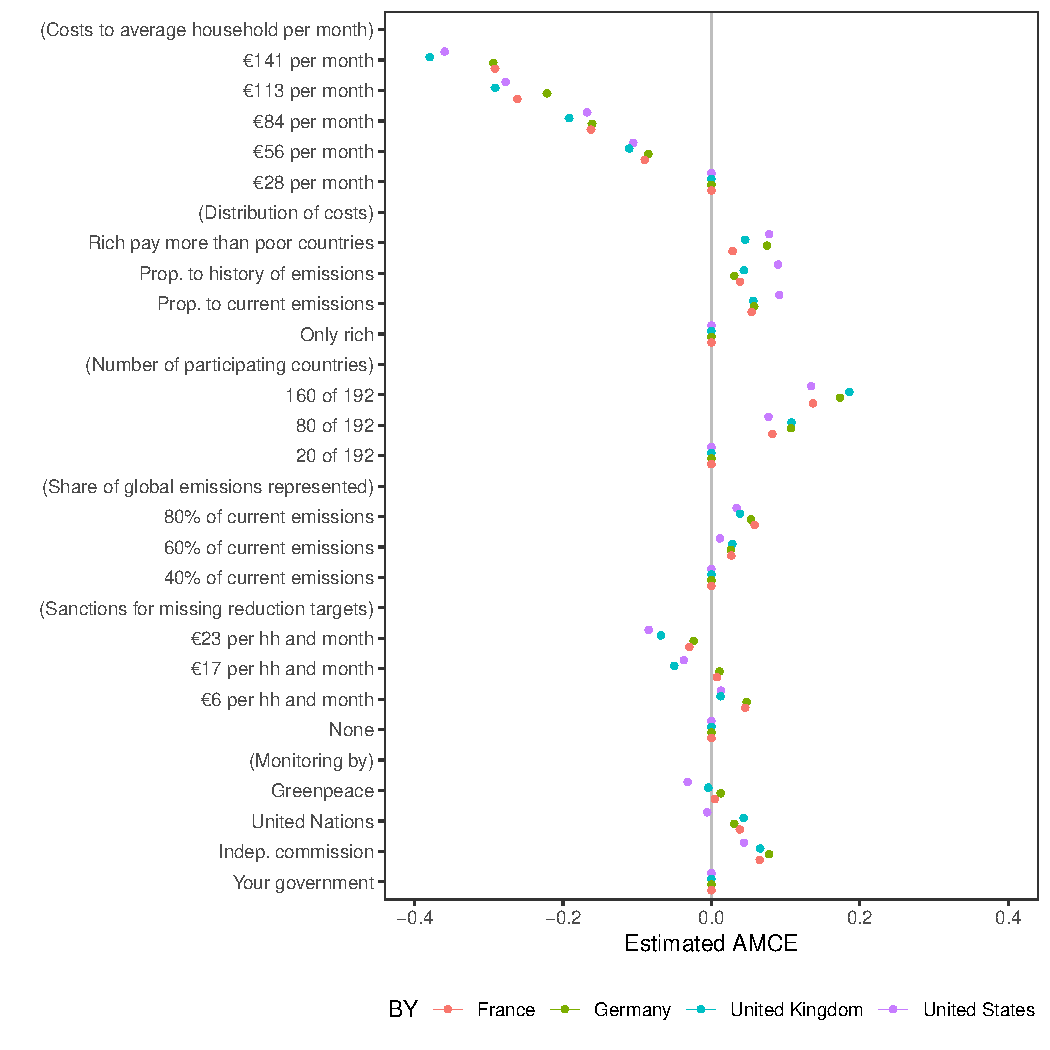
\includegraphics[width=\maxwidth]{figure/bechtel_subgroup_amce-1} 
\begin{kframe}\begin{verbatim}
##                BY   outcome statistic
## 1          France choice_cj      amce
## 2          France choice_cj      amce
## 3          France choice_cj      amce
## 4          France choice_cj      amce
## 5          France choice_cj      amce
## 6          France choice_cj      amce
## 7          France choice_cj      amce
## 8          France choice_cj      amce
## 9          France choice_cj      amce
## 10         France choice_cj      amce
## 11         France choice_cj      amce
## 12         France choice_cj      amce
## 13         France choice_cj      amce
## 14         France choice_cj      amce
## 15         France choice_cj      amce
## 16         France choice_cj      amce
## 17         France choice_cj      amce
## 18         France choice_cj      amce
## 19         France choice_cj      amce
## 20         France choice_cj      amce
## 21         France choice_cj      amce
## 22         France choice_cj      amce
## 23         France choice_cj      amce
## 24        Germany choice_cj      amce
## 25        Germany choice_cj      amce
## 26        Germany choice_cj      amce
## 27        Germany choice_cj      amce
## 28        Germany choice_cj      amce
## 29        Germany choice_cj      amce
## 30        Germany choice_cj      amce
## 31        Germany choice_cj      amce
## 32        Germany choice_cj      amce
## 33        Germany choice_cj      amce
## 34        Germany choice_cj      amce
## 35        Germany choice_cj      amce
## 36        Germany choice_cj      amce
## 37        Germany choice_cj      amce
## 38        Germany choice_cj      amce
## 39        Germany choice_cj      amce
## 40        Germany choice_cj      amce
## 41        Germany choice_cj      amce
## 42        Germany choice_cj      amce
## 43        Germany choice_cj      amce
## 44        Germany choice_cj      amce
## 45        Germany choice_cj      amce
## 46        Germany choice_cj      amce
## 47 United Kingdom choice_cj      amce
## 48 United Kingdom choice_cj      amce
## 49 United Kingdom choice_cj      amce
## 50 United Kingdom choice_cj      amce
## 51 United Kingdom choice_cj      amce
## 52 United Kingdom choice_cj      amce
## 53 United Kingdom choice_cj      amce
## 54 United Kingdom choice_cj      amce
## 55 United Kingdom choice_cj      amce
## 56 United Kingdom choice_cj      amce
## 57 United Kingdom choice_cj      amce
## 58 United Kingdom choice_cj      amce
## 59 United Kingdom choice_cj      amce
## 60 United Kingdom choice_cj      amce
## 61 United Kingdom choice_cj      amce
## 62 United Kingdom choice_cj      amce
## 63 United Kingdom choice_cj      amce
## 64 United Kingdom choice_cj      amce
## 65 United Kingdom choice_cj      amce
## 66 United Kingdom choice_cj      amce
## 67 United Kingdom choice_cj      amce
## 68 United Kingdom choice_cj      amce
## 69 United Kingdom choice_cj      amce
## 70  United States choice_cj      amce
## 71  United States choice_cj      amce
## 72  United States choice_cj      amce
## 73  United States choice_cj      amce
## 74  United States choice_cj      amce
## 75  United States choice_cj      amce
## 76  United States choice_cj      amce
## 77  United States choice_cj      amce
## 78  United States choice_cj      amce
## 79  United States choice_cj      amce
## 80  United States choice_cj      amce
## 81  United States choice_cj      amce
## 82  United States choice_cj      amce
## 83  United States choice_cj      amce
## 84  United States choice_cj      amce
## 85  United States choice_cj      amce
## 86  United States choice_cj      amce
## 87  United States choice_cj      amce
## 88  United States choice_cj      amce
## 89  United States choice_cj      amce
## 90  United States choice_cj      amce
## 91  United States choice_cj      amce
## 92  United States choice_cj      amce
##                                    feature
## 1     Costs to average household per month
## 2     Costs to average household per month
## 3     Costs to average household per month
## 4     Costs to average household per month
## 5     Costs to average household per month
## 6                    Distribution of costs
## 7                    Distribution of costs
## 8                    Distribution of costs
## 9                    Distribution of costs
## 10       Number of participating countries
## 11       Number of participating countries
## 12       Number of participating countries
## 13   Share of global emissions represented
## 14   Share of global emissions represented
## 15   Share of global emissions represented
## 16 Sanctions for missing reduction targets
## 17 Sanctions for missing reduction targets
## 18 Sanctions for missing reduction targets
## 19 Sanctions for missing reduction targets
## 20                           Monitoring by
## 21                           Monitoring by
## 22                           Monitoring by
## 23                           Monitoring by
## 24    Costs to average household per month
## 25    Costs to average household per month
## 26    Costs to average household per month
## 27    Costs to average household per month
## 28    Costs to average household per month
## 29                   Distribution of costs
## 30                   Distribution of costs
## 31                   Distribution of costs
## 32                   Distribution of costs
## 33       Number of participating countries
## 34       Number of participating countries
## 35       Number of participating countries
## 36   Share of global emissions represented
## 37   Share of global emissions represented
## 38   Share of global emissions represented
## 39 Sanctions for missing reduction targets
## 40 Sanctions for missing reduction targets
## 41 Sanctions for missing reduction targets
## 42 Sanctions for missing reduction targets
## 43                           Monitoring by
## 44                           Monitoring by
## 45                           Monitoring by
## 46                           Monitoring by
## 47    Costs to average household per month
## 48    Costs to average household per month
## 49    Costs to average household per month
## 50    Costs to average household per month
## 51    Costs to average household per month
## 52                   Distribution of costs
## 53                   Distribution of costs
## 54                   Distribution of costs
## 55                   Distribution of costs
## 56       Number of participating countries
## 57       Number of participating countries
## 58       Number of participating countries
## 59   Share of global emissions represented
## 60   Share of global emissions represented
## 61   Share of global emissions represented
## 62 Sanctions for missing reduction targets
## 63 Sanctions for missing reduction targets
## 64 Sanctions for missing reduction targets
## 65 Sanctions for missing reduction targets
## 66                           Monitoring by
## 67                           Monitoring by
## 68                           Monitoring by
## 69                           Monitoring by
## 70    Costs to average household per month
## 71    Costs to average household per month
## 72    Costs to average household per month
## 73    Costs to average household per month
## 74    Costs to average household per month
## 75                   Distribution of costs
## 76                   Distribution of costs
## 77                   Distribution of costs
## 78                   Distribution of costs
## 79       Number of participating countries
## 80       Number of participating countries
## 81       Number of participating countries
## 82   Share of global emissions represented
## 83   Share of global emissions represented
## 84   Share of global emissions represented
## 85 Sanctions for missing reduction targets
## 86 Sanctions for missing reduction targets
## 87 Sanctions for missing reduction targets
## 88 Sanctions for missing reduction targets
## 89                           Monitoring by
## 90                           Monitoring by
## 91                           Monitoring by
## 92                           Monitoring by
##                                level     estimate   std.error           z
## 1                      \20028 per month  0.000000000          NA          NA
## 2                      \20056 per month -0.089860961 0.002813351  -31.940905
## 3                      \20084 per month -0.162436163 0.002934504  -55.353875
## 4                     \200113 per month -0.261547555 0.002918526  -89.616324
## 5                     \200141 per month -0.291645421 0.002902892 -100.467203
## 6                          Only rich  0.000000000          NA          NA
## 7         Prop. to current emissions  0.054200226 0.002607077   20.789650
## 8      Prop. to history of emissions  0.038328103 0.002658713   14.416038
## 9  Rich pay more than poor countries  0.028519774 0.002646147   10.777849
## 10                         20 of 192  0.000000000          NA          NA
## 11                         80 of 192  0.082106285 0.002229365   36.829446
## 12                        160 of 192  0.136730466 0.002294899   59.580169
## 13          40% of current emissions  0.000000000          NA          NA
## 14          60% of current emissions  0.026854567 0.002215284   12.122401
## 15          80% of current emissions  0.058282940 0.002221222   26.239130
## 16                              None  0.000000000          NA          NA
## 17               \2006 per hh and month  0.045613729 0.002581015   17.672790
## 18              \20017 per hh and month  0.007229382 0.002610090    2.769783
## 19              \20023 per hh and month -0.029804720 0.002632489  -11.321878
## 20                   Your government  0.000000000          NA          NA
## 21                 Indep. commission  0.065056568 0.002580643   25.209438
## 22                    United Nations  0.038172745 0.002649490   14.407580
## 23                        Greenpeace  0.004689020 0.002607562    1.798239
## 24                     \20028 per month  0.000000000          NA          NA
## 25                     \20056 per month -0.084977509 0.002750651  -30.893604
## 26                     \20084 per month -0.160748210 0.002916213  -55.122247
## 27                    \200113 per month -0.221878444 0.002925864  -75.833469
## 28                    \200141 per month -0.294163816 0.002844194 -103.426084
## 29                         Only rich  0.000000000          NA          NA
## 30        Prop. to current emissions  0.057662754 0.002699207   21.362849
## 31     Prop. to history of emissions  0.030679640 0.002714117   11.303730
## 32 Rich pay more than poor countries  0.074927931 0.002679618   27.962166
## 33                         20 of 192  0.000000000          NA          NA
## 34                         80 of 192  0.107154481 0.002265078   47.307193
## 35                        160 of 192  0.173181493 0.002384032   72.642272
## 36          40% of current emissions  0.000000000          NA          NA
## 37          60% of current emissions  0.026132954 0.002205416   11.849446
## 38          80% of current emissions  0.053053884 0.002258783   23.487818
## 39                              None  0.000000000          NA          NA
## 40               \2006 per hh and month  0.047406399 0.002648398   17.900028
## 41              \20017 per hh and month  0.010933985 0.002724889    4.012635
## 42              \20023 per hh and month -0.023959166 0.002638535   -9.080480
## 43                   Your government  0.000000000          NA          NA
## 44                 Indep. commission  0.077729780 0.002653729   29.290775
## 45                    United Nations  0.030758786 0.002624494   11.719893
## 46                        Greenpeace  0.012420581 0.002770108    4.483790
## 47                     \20028 per month  0.000000000          NA          NA
## 48                     \20056 per month -0.110733022 0.002903505  -38.137711
## 49                     \20084 per month -0.191782558 0.003027556  -63.345665
## 50                    \200113 per month -0.291316540 0.003078639  -94.625104
## 51                    \200141 per month -0.379787694 0.002882191 -131.770492
## 52                         Only rich  0.000000000          NA          NA
## 53        Prop. to current emissions  0.056480847 0.002812594   20.081409
## 54     Prop. to history of emissions  0.043676581 0.002797188   15.614462
## 55 Rich pay more than poor countries  0.045401046 0.002744631   16.541766
## 56                         20 of 192  0.000000000          NA          NA
## 57                         80 of 192  0.107780809 0.002389605   45.104030
## 58                        160 of 192  0.185987301 0.002431676   76.485226
## 59          40% of current emissions  0.000000000          NA          NA
## 60          60% of current emissions  0.028210800 0.002319342   12.163279
## 61          80% of current emissions  0.038497022 0.002344981   16.416773
## 62                              None  0.000000000          NA          NA
## 63               \2006 per hh and month  0.012309687 0.002686688    4.581734
## 64              \20017 per hh and month -0.050191678 0.002702107  -18.575015
## 65              \20023 per hh and month -0.068078009 0.002704177  -25.175133
## 66                   Your government  0.000000000          NA          NA
## 67                 Indep. commission  0.065661468 0.002759607   23.793775
## 68                    United Nations  0.043434121 0.002756915   15.754611
## 69                        Greenpeace -0.004138694 0.002912058   -1.421227
## 70                     \20028 per month  0.000000000          NA          NA
## 71                     \20056 per month -0.105444490 0.002702673  -39.014884
## 72                     \20084 per month -0.167525238 0.002834364  -59.105046
## 73                    \200113 per month -0.277525944 0.002803157  -99.004768
## 74                    \200141 per month -0.359605089 0.002680793 -134.141324
## 75                         Only rich  0.000000000          NA          NA
## 76        Prop. to current emissions  0.091203284 0.002550920   35.753099
## 77     Prop. to history of emissions  0.090070483 0.002543861   35.407003
## 78 Rich pay more than poor countries  0.077781900 0.002504744   31.053829
## 79                         20 of 192  0.000000000          NA          NA
## 80                         80 of 192  0.076940577 0.002208008   34.846146
## 81                        160 of 192  0.134596041 0.002248790   59.852638
## 82          40% of current emissions  0.000000000          NA          NA
## 83          60% of current emissions  0.011423002 0.002160677    5.286770
## 84          80% of current emissions  0.033988555 0.002148874   15.816911
## 85                              None  0.000000000          NA          NA
## 86               \2006 per hh and month  0.012594565 0.002518411    5.000996
## 87              \20017 per hh and month -0.037280077 0.002515684  -14.819060
## 88              \20023 per hh and month -0.084672056 0.002479801  -34.144695
## 89                   Your government  0.000000000          NA          NA
## 90                 Indep. commission  0.043987035 0.002548830   17.257734
## 91                    United Nations -0.005622035 0.002735205   -2.055435
## 92                        Greenpeace -0.032025463 0.002673662  -11.978126
##                p         lower         upper        country
## 1             NA            NA            NA         France
## 2  7.226159e-224 -0.0953750271 -0.0843468956         France
## 3   0.000000e+00 -0.1681876847 -0.1566846408         France
## 4   0.000000e+00 -0.2672677610 -0.2558273500         France
## 5   0.000000e+00 -0.2973349846 -0.2859558578         France
## 6             NA            NA            NA         France
## 7   5.370116e-96  0.0490904481  0.0593100036         France
## 8   4.102248e-47  0.0331171221  0.0435390844         France
## 9   4.380069e-27  0.0233334208  0.0337061265         France
## 10            NA            NA            NA         France
## 11 6.239429e-297  0.0777368097  0.0864757606         France
## 12  0.000000e+00  0.1322325464  0.1412283848         France
## 13            NA            NA            NA         France
## 14  8.036931e-34  0.0225126894  0.0311964449         France
## 15 9.511109e-152  0.0539294246  0.0626364558         France
## 16            NA            NA            NA         France
## 17  6.795136e-70  0.0405550330  0.0506724242         France
## 18  5.609365e-03  0.0021137003  0.0123450641         France
## 19  1.022571e-29 -0.0349643037 -0.0246451365         France
## 20            NA            NA            NA         France
## 21 3.156501e-140  0.0599985998  0.0701145359         France
## 22  4.636712e-47  0.0329798393  0.0433656505         France
## 23  7.213906e-02 -0.0004217066  0.0097997474         France
## 24            NA            NA            NA        Germany
## 25 1.455731e-209 -0.0903686852 -0.0795863332        Germany
## 26  0.000000e+00 -0.1664638827 -0.1550325381        Germany
## 27  0.000000e+00 -0.2276130332 -0.2161438557        Germany
## 28  0.000000e+00 -0.2997383334 -0.2885892990        Germany
## 29            NA            NA            NA        Germany
## 30 2.961840e-101  0.0523724056  0.0629531032        Germany
## 31  1.257611e-29  0.0253600694  0.0359992110        Germany
## 32 4.689630e-172  0.0696759757  0.0801798863        Germany
## 33            NA            NA            NA        Germany
## 34  0.000000e+00  0.1027150093  0.1115939518        Germany
## 35  0.000000e+00  0.1685088765  0.1778541098        Germany
## 36            NA            NA            NA        Germany
## 37  2.166183e-32  0.0218104185  0.0304554892        Germany
## 38 5.433027e-122  0.0486267509  0.0574810175        Germany
## 39            NA            NA            NA        Germany
## 40  1.178625e-71  0.0422156343  0.0525971638        Germany
## 41  6.004460e-05  0.0055933013  0.0162746686        Germany
## 42  1.080972e-19 -0.0291306001 -0.0187877321        Germany
## 43            NA            NA            NA        Germany
## 44 1.359389e-188  0.0725285663  0.0829309931        Germany
## 45  1.007986e-31  0.0256148727  0.0359026987        Germany
## 46  7.332889e-06  0.0069912698  0.0178498930        Germany
## 47            NA            NA            NA United Kingdom
## 48  0.000000e+00 -0.1164237867 -0.1050422575 United Kingdom
## 49  0.000000e+00 -0.1977164589 -0.1858486569 United Kingdom
## 50  0.000000e+00 -0.2973505613 -0.2852825180 United Kingdom
## 51  0.000000e+00 -0.3854366842 -0.3741387041 United Kingdom
## 52            NA            NA            NA United Kingdom
## 53  1.073077e-89  0.0509682645  0.0619934297 United Kingdom
## 54  5.803241e-55  0.0381941936  0.0491589676 United Kingdom
## 55  1.835610e-61  0.0400216677  0.0507804240 United Kingdom
## 56            NA            NA            NA United Kingdom
## 57  0.000000e+00  0.1030972691  0.1124643479 United Kingdom
## 58  0.000000e+00  0.1812213035  0.1907532989 United Kingdom
## 59            NA            NA            NA United Kingdom
## 60  4.876126e-34  0.0236649738  0.0327566260 United Kingdom
## 61  1.450801e-60  0.0339009438  0.0430931007 United Kingdom
## 62            NA            NA            NA United Kingdom
## 63  4.611371e-06  0.0070438759  0.0175754978 United Kingdom
## 64  5.119048e-77 -0.0554877102 -0.0448956456 United Kingdom
## 65 7.501029e-140 -0.0733780984 -0.0627779202 United Kingdom
## 66            NA            NA            NA United Kingdom
## 67 3.874082e-125  0.0602527374  0.0710701983 United Kingdom
## 68  6.385102e-56  0.0380306668  0.0488375744 United Kingdom
## 69  1.552509e-01 -0.0098462235  0.0015688348 United Kingdom
## 70            NA            NA            NA  United States
## 71  0.000000e+00 -0.1107416331 -0.1001473479  United States
## 72  0.000000e+00 -0.1730804906 -0.1619699863  United States
## 73  0.000000e+00 -0.2830200319 -0.2720318569  United States
## 74  0.000000e+00 -0.3648593460 -0.3543508315  United States
## 75            NA            NA            NA  United States
## 76 5.921344e-280  0.0862035730  0.0962029943  United States
## 77 1.332257e-274  0.0850846075  0.0950563580  United States
## 78 1.012831e-211  0.0728726920  0.0826911090  United States
## 79            NA            NA            NA  United States
## 80 4.870184e-266  0.0726129606  0.0812681938  United States
## 81  0.000000e+00  0.1301884926  0.1390035893  United States
## 82            NA            NA            NA  United States
## 83  1.244952e-07  0.0071881530  0.0156578517  United States
## 84  2.378815e-56  0.0297768386  0.0382002715  United States
## 85            NA            NA            NA  United States
## 86  5.703489e-07  0.0076585697  0.0175305610  United States
## 87  1.103176e-49 -0.0422107276 -0.0323494261  United States
## 88 1.602925e-255 -0.0895323769 -0.0798117349  United States
## 89            NA            NA            NA  United States
## 90  9.787681e-67  0.0389914198  0.0489826509  United States
## 91  3.983702e-02 -0.0109829381 -0.0002611325  United States
## 92  4.626637e-33 -0.0372657443 -0.0267851811  United States
\end{verbatim}
\end{kframe}
\end{knitrout}

\begin{knitrout}
\definecolor{shadecolor}{rgb}{0.969, 0.969, 0.969}\color{fgcolor}\begin{kframe}
\begin{verbatim}
## Analysis of Deviance Table
## 
## Model 1: choice_cj ~ cost_cj + distrib_cj + ctries_cj + emissions_cj + 
##     sanctions_cj + monitoring_cj
## Model 2: choice_cj ~ cost_cj + distrib_cj + ctries_cj + emissions_cj + 
##     sanctions_cj + monitoring_cj + country + cost_cj:country + 
##     distrib_cj:country + ctries_cj:country + emissions_cj:country + 
##     sanctions_cj:country + monitoring_cj:country
##   Resid. Df Resid. Dev Df Deviance      F    Pr(>F)    
## 1     67982      15601                                 
## 2     67928      15555 54   45.983 3.7187 < 2.2e-16 ***
## ---
## Signif. codes:  0 '***' 0.001 '**' 0.01 '*' 0.05 '.' 0.1 ' ' 1
\end{verbatim}
\end{kframe}
\end{knitrout}


\begin{knitrout}
\definecolor{shadecolor}{rgb}{0.969, 0.969, 0.969}\color{fgcolor}
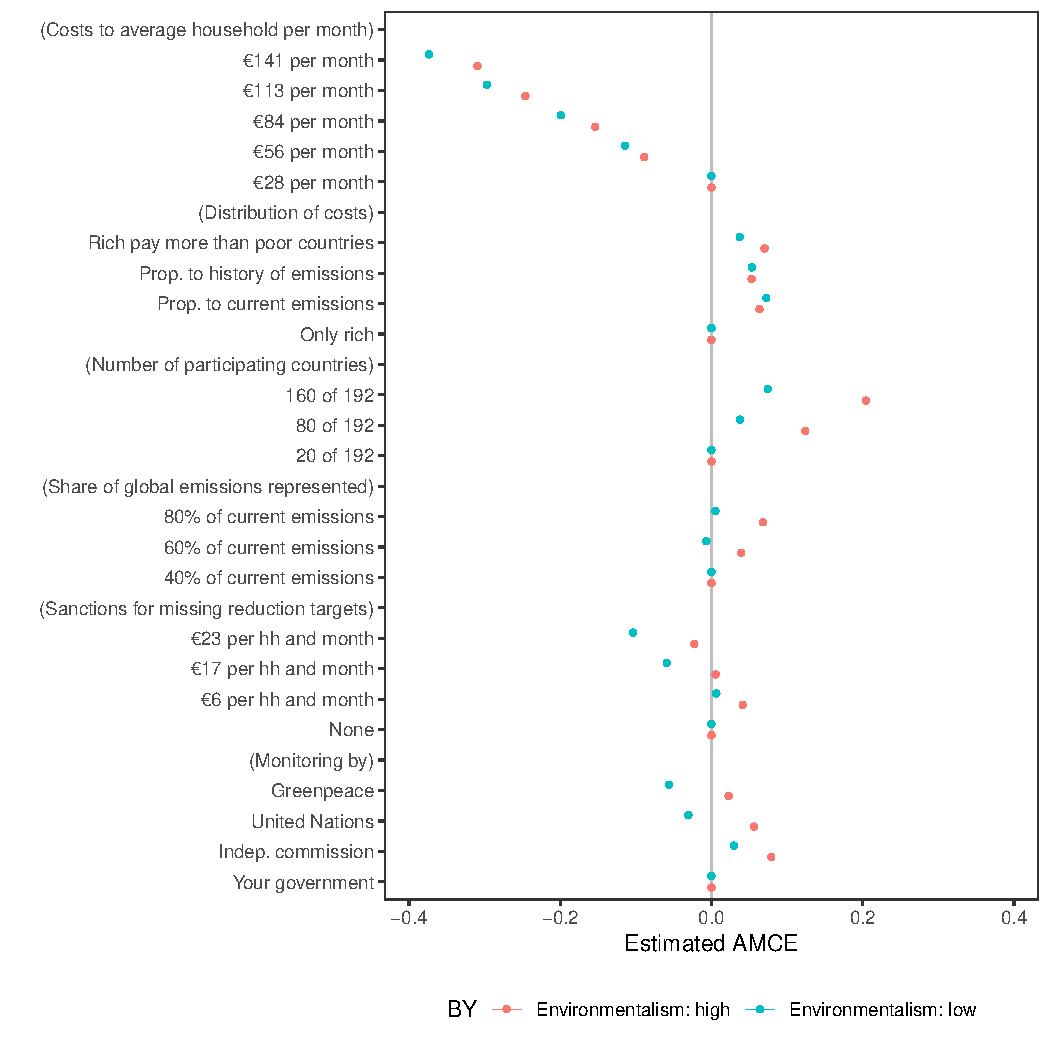
\includegraphics[width=\maxwidth]{figure/bechtel_subgroup_amce_environmentalism-1} 

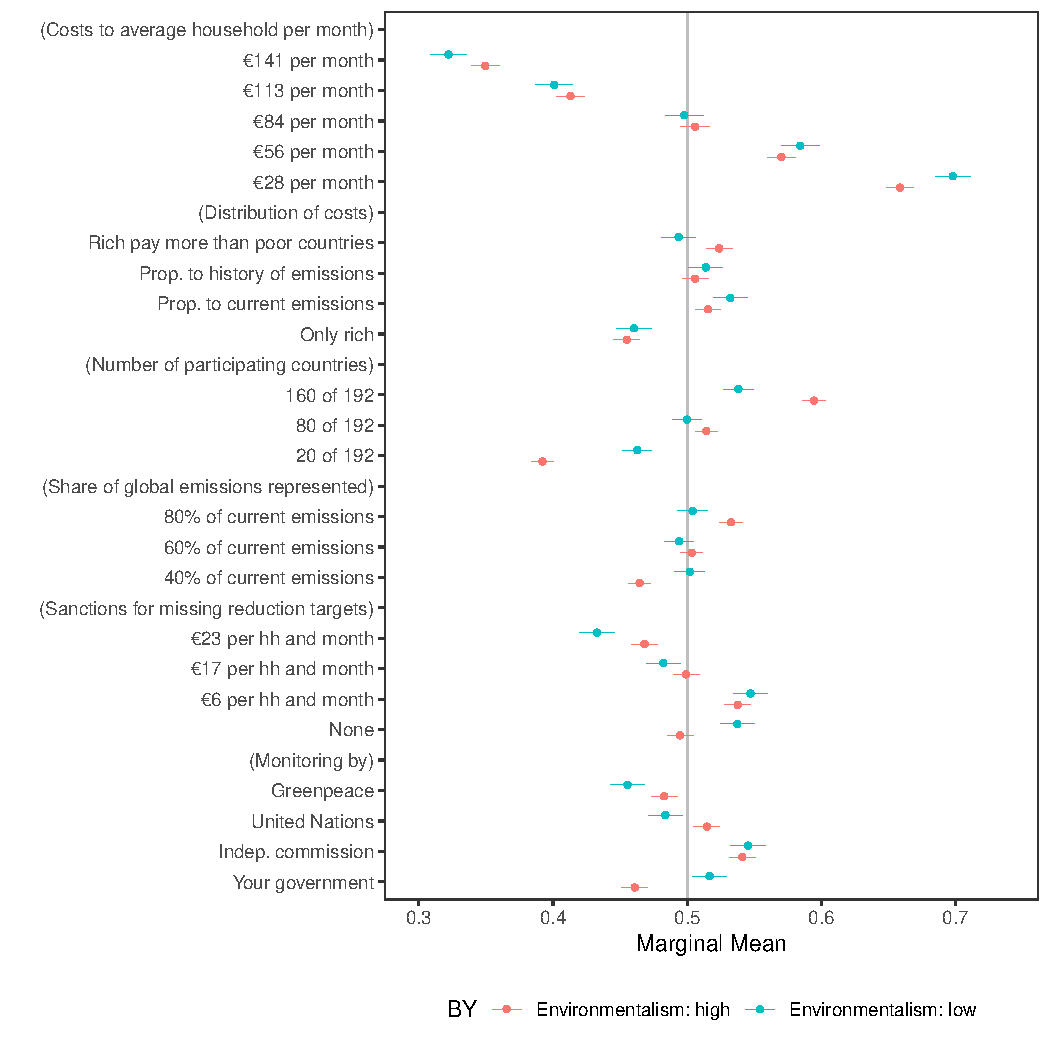
\includegraphics[width=\maxwidth]{figure/bechtel_subgroup_amce_environmentalism-2} 

\end{knitrout}



\begin{knitrout}
\definecolor{shadecolor}{rgb}{0.969, 0.969, 0.969}\color{fgcolor}
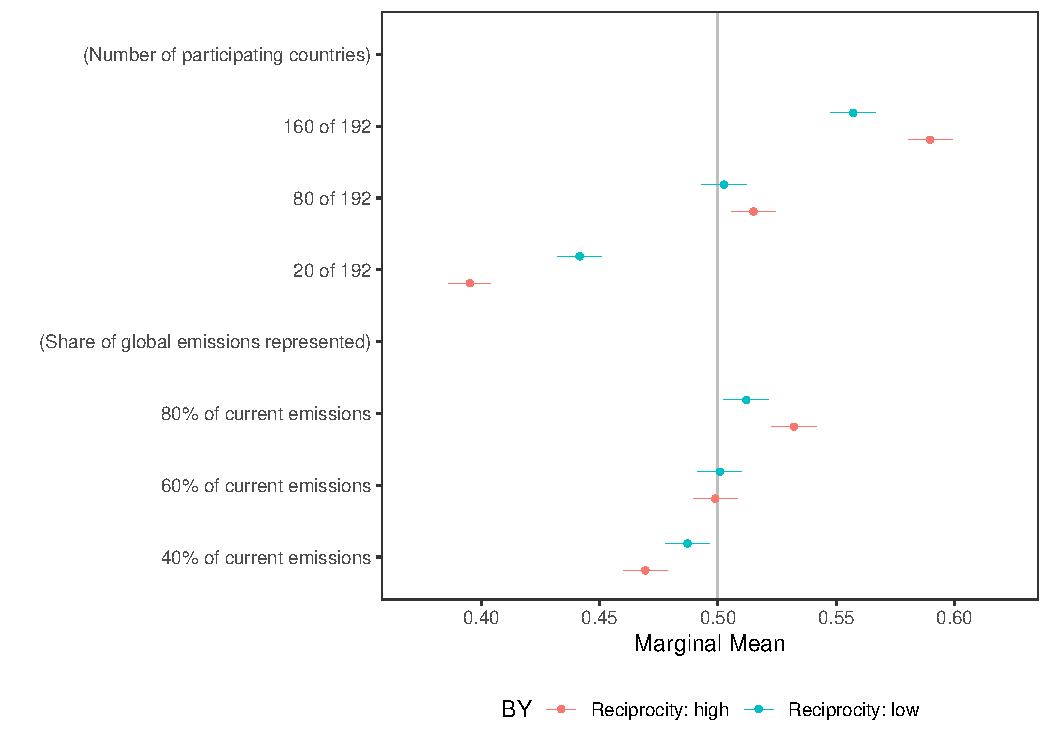
\includegraphics[width=\maxwidth]{figure/bechtel_reciprocity_reference-1} 

\end{knitrout}


\begin{knitrout}
\definecolor{shadecolor}{rgb}{0.969, 0.969, 0.969}\color{fgcolor}
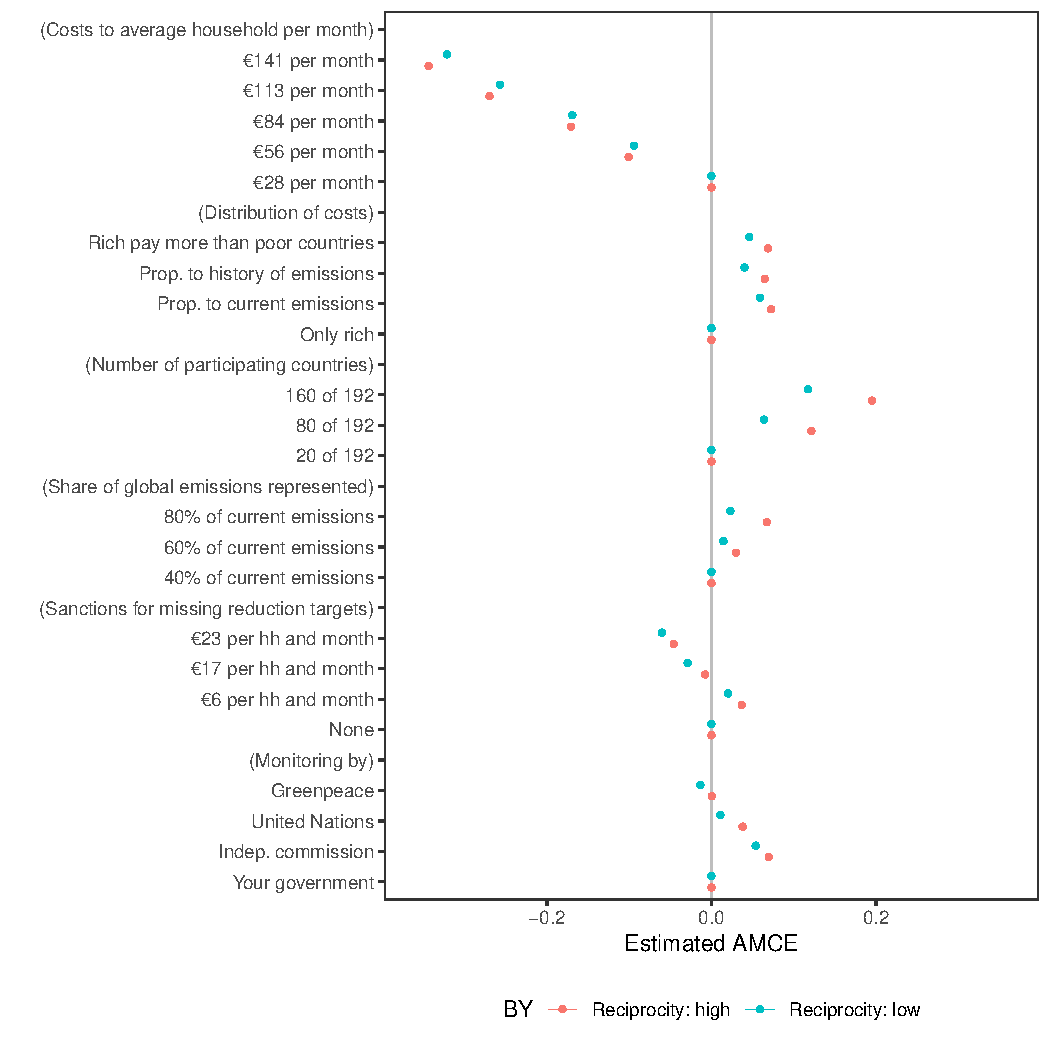
\includegraphics[width=\maxwidth]{figure/bechtel_subgroup_amce_reciprocity-1} 

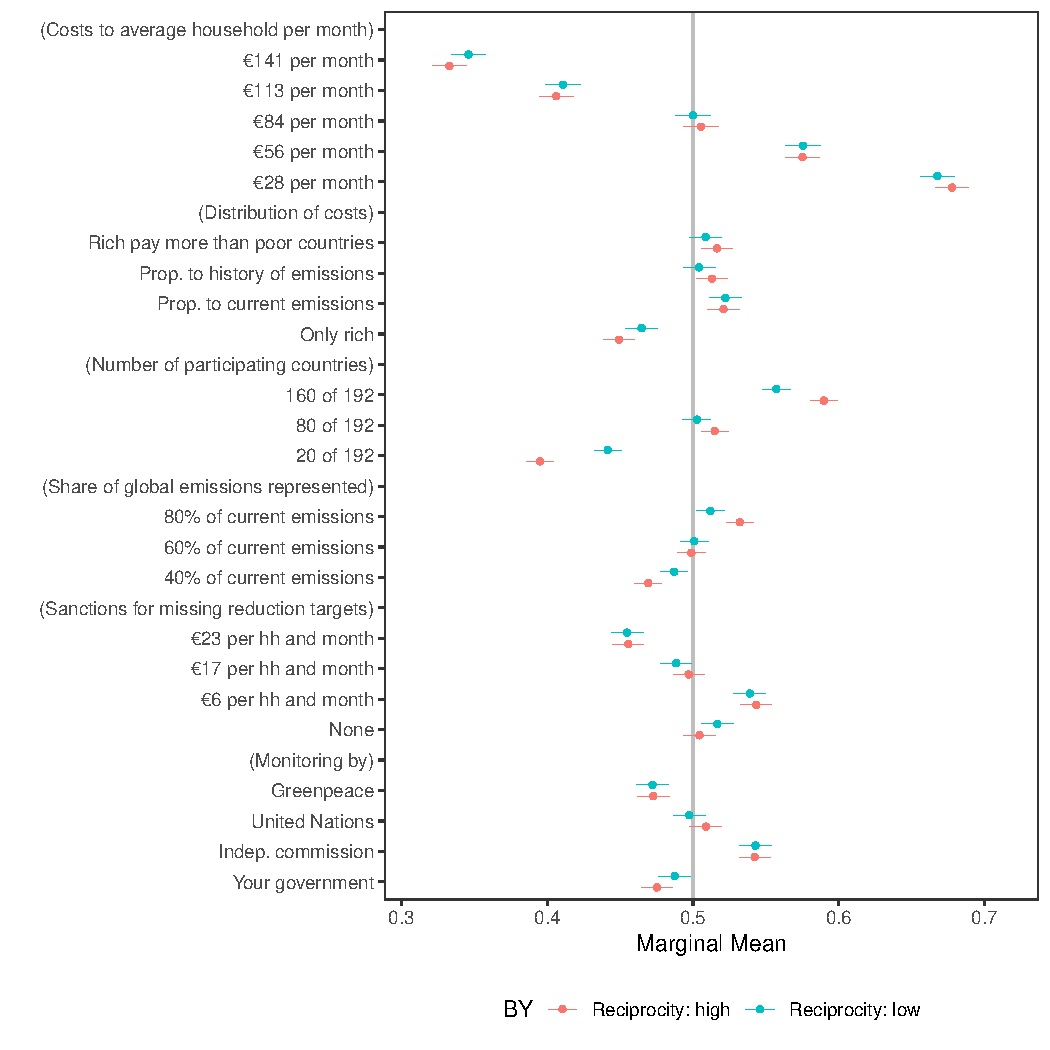
\includegraphics[width=\maxwidth]{figure/bechtel_subgroup_amce_reciprocity-2} 

\end{knitrout}


\clearpage








\section{Teele et al. (2018) Candidate Experiment}

\subsection{Replication using AMCEs}

\begin{knitrout}
\definecolor{shadecolor}{rgb}{0.969, 0.969, 0.969}\color{fgcolor}
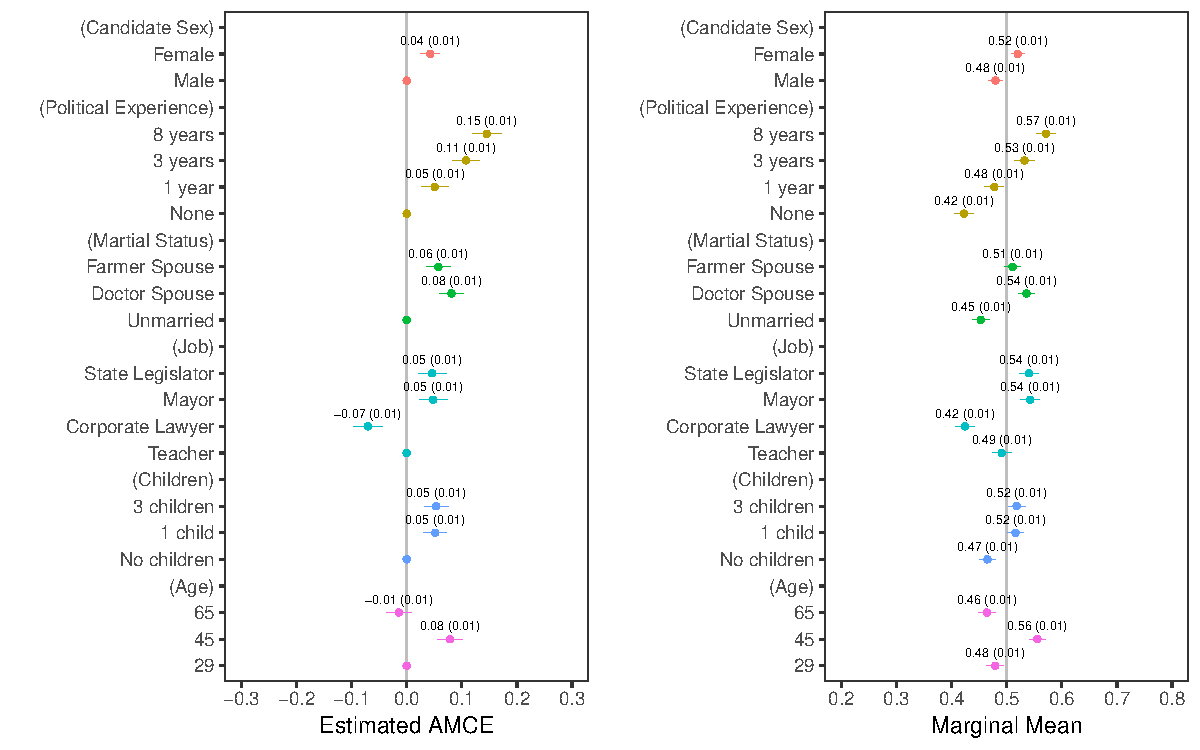
\includegraphics[width=\maxwidth]{figure/tkr_amce_appendix-1} 

\end{knitrout}

\clearpage

% latex table generated in R 3.5.1 by xtable 1.8-3 package
% Sun Nov 25 10:43:16 2018
\begin{table}[ht]
\centering
\begin{tabular}{lp{1.5in}rrr}
  \hline
feature & level & estimate & std.error & z \\ 
  \hline
Candidate Sex & Male & 0.00 &  &  \\ 
  Candidate Sex & Female & 0.04 & 0.01 & 4.74 \\ 
  Political Experience & None & 0.00 &  &  \\ 
  Political Experience & 1 year & 0.05 & 0.01 & 4.06 \\ 
  Political Experience & 3 years & 0.11 & 0.01 & 8.47 \\ 
  Political Experience & 8 years & 0.15 & 0.01 & 10.83 \\ 
  Martial Status & Unmarried & 0.00 &  &  \\ 
  Martial Status & Doctor Spouse & 0.08 & 0.01 & 7.25 \\ 
  Martial Status & Farmer Spouse & 0.06 & 0.01 & 5.26 \\ 
  Job & Teacher & 0.00 &  &  \\ 
  Job & Corporate Lawyer & -0.07 & 0.01 & -5.29 \\ 
  Job & Mayor & 0.05 & 0.01 & 3.74 \\ 
  Job & State Legislator & 0.05 & 0.01 & 3.59 \\ 
  Children & No children & 0.00 &  &  \\ 
  Children & 1 child & 0.05 & 0.01 & 4.84 \\ 
  Children & 3 children & 0.05 & 0.01 & 4.77 \\ 
  Age & 29 & 0.00 &  &  \\ 
  Age & 45 & 0.08 & 0.01 & 7.07 \\ 
  Age & 65 & -0.01 & 0.01 & -1.24 \\ 
   \hline
\end{tabular}
\end{table}


\clearpage

\subsection{Replication using MMs}

\begin{knitrout}
\definecolor{shadecolor}{rgb}{0.969, 0.969, 0.969}\color{fgcolor}
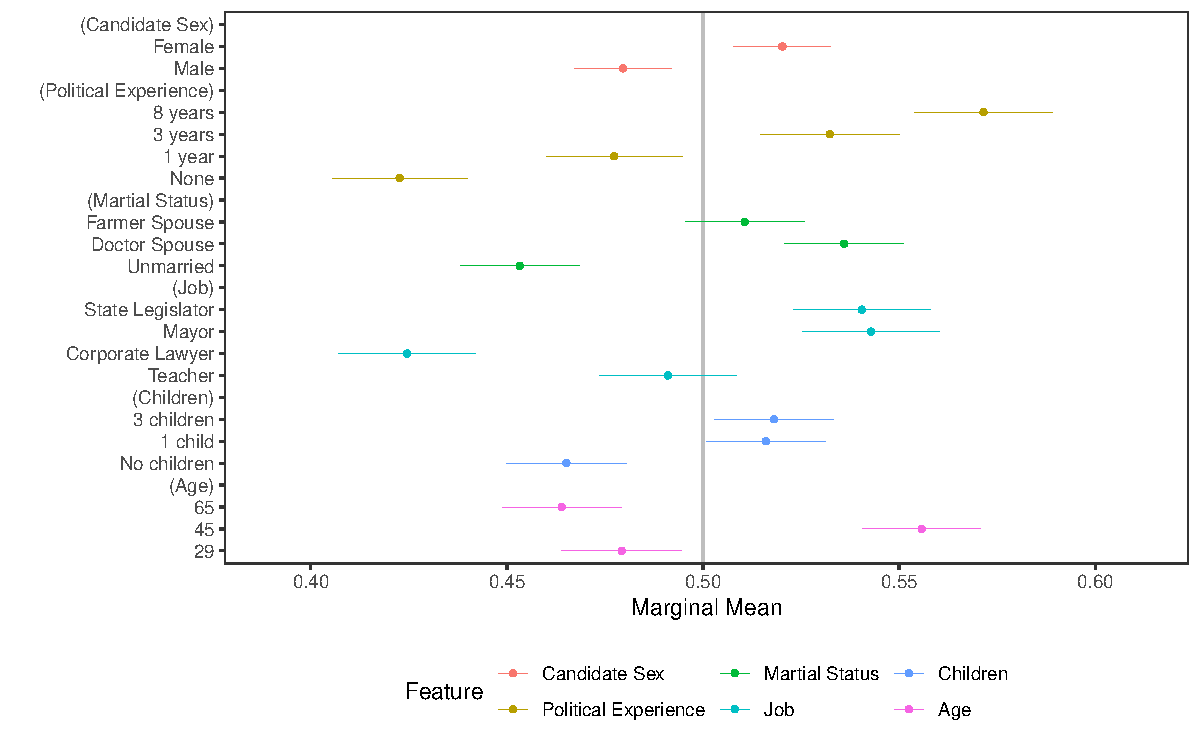
\includegraphics[width=\maxwidth]{figure/tkr_mm_appendix-1} 

\end{knitrout}

\clearpage

% latex table generated in R 3.5.1 by xtable 1.8-3 package
% Sun Nov 25 10:43:19 2018
\begin{table}[ht]
\centering
\begin{tabular}{lp{1.5in}rrr}
  \hline
feature & level & estimate & std.error & z \\ 
  \hline
Candidate Sex & Male & 0.48 & 0.01 & -3.22 \\ 
  Candidate Sex & Female & 0.52 & 0.01 & 3.20 \\ 
  Political Experience & None & 0.42 & 0.01 & -8.81 \\ 
  Political Experience & 1 year & 0.48 & 0.01 & -2.56 \\ 
  Political Experience & 3 years & 0.53 & 0.01 & 3.58 \\ 
  Political Experience & 8 years & 0.57 & 0.01 & 7.99 \\ 
  Martial Status & Unmarried & 0.45 & 0.01 & -6.05 \\ 
  Martial Status & Doctor Spouse & 0.54 & 0.01 & 4.66 \\ 
  Martial Status & Farmer Spouse & 0.51 & 0.01 & 1.37 \\ 
  Job & Teacher & 0.49 & 0.01 & -1.01 \\ 
  Job & Corporate Lawyer & 0.42 & 0.01 & -8.44 \\ 
  Job & Mayor & 0.54 & 0.01 & 4.77 \\ 
  Job & State Legislator & 0.54 & 0.01 & 4.55 \\ 
  Children & No children & 0.47 & 0.01 & -4.47 \\ 
  Children & 1 child & 0.52 & 0.01 & 2.07 \\ 
  Children & 3 children & 0.52 & 0.01 & 2.34 \\ 
  Age & 29 & 0.48 & 0.01 & -2.65 \\ 
  Age & 45 & 0.56 & 0.01 & 7.28 \\ 
  Age & 65 & 0.46 & 0.01 & -4.66 \\ 
   \hline
\end{tabular}
\end{table}


\clearpage

\subsection{Subgroup Analysis for Teele et al. (2018) Candidate Experiment using AMCEs}

\begin{knitrout}
\definecolor{shadecolor}{rgb}{0.969, 0.969, 0.969}\color{fgcolor}
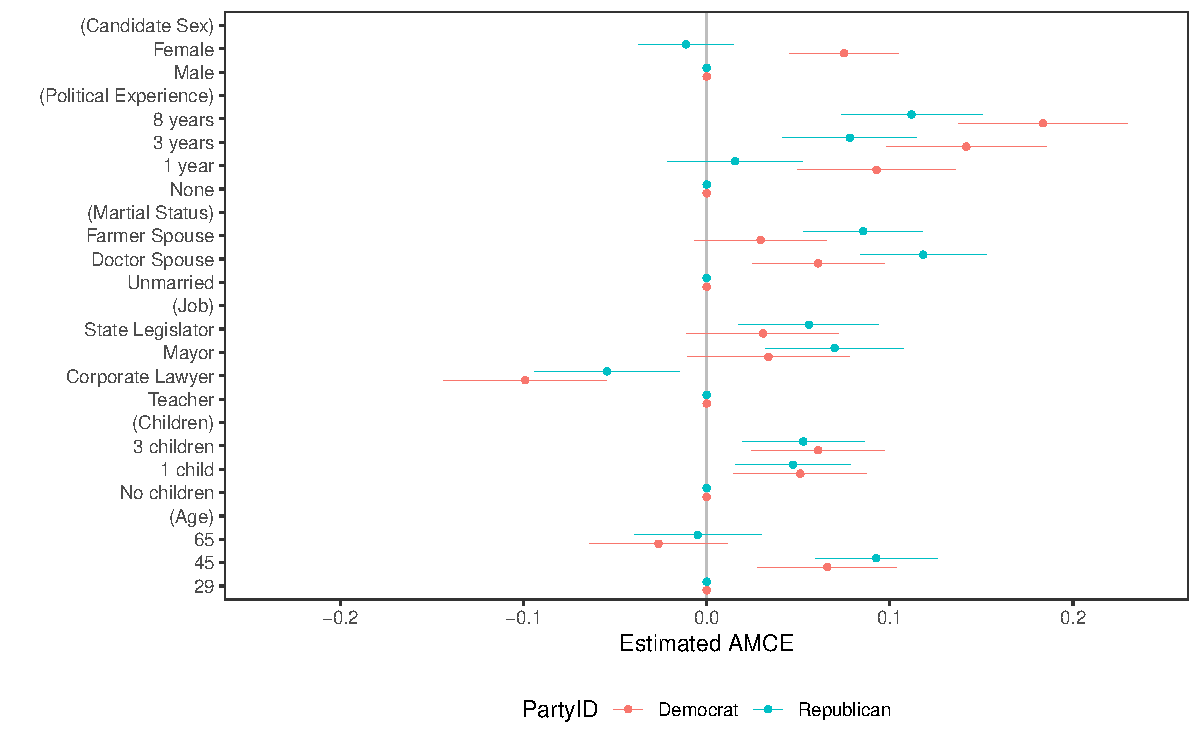
\includegraphics[width=\maxwidth]{figure/tkr_subgroup_amce_appendix-1} 

\end{knitrout}

\subsection{Subgroup Analysis for Teele et al. (2018) Candidate Experiment using MMs}

\begin{knitrout}
\definecolor{shadecolor}{rgb}{0.969, 0.969, 0.969}\color{fgcolor}
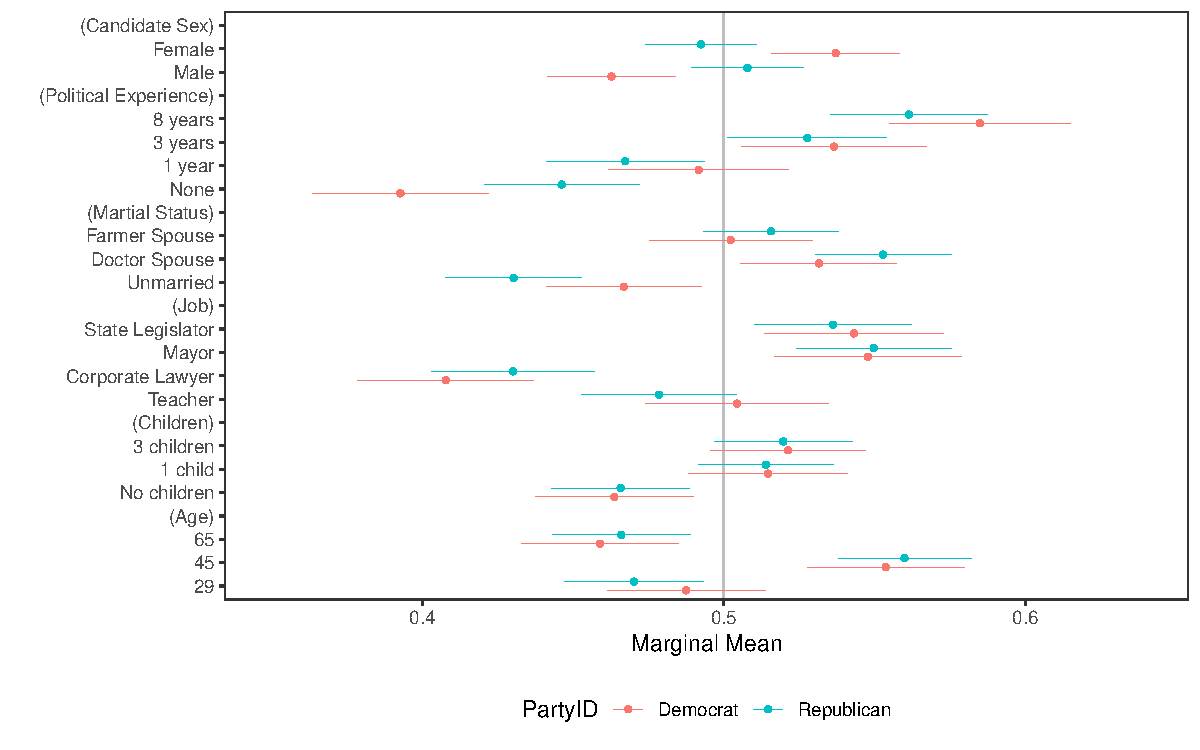
\includegraphics[width=\maxwidth]{figure/tkr_subgroup_mm_appendix-1} 

\end{knitrout}

\clearpage

\subsection{Comparison of Alternative Reference Categories for Teele et al. (2018) Candidate Experiment}




\begin{knitrout}
\definecolor{shadecolor}{rgb}{0.969, 0.969, 0.969}\color{fgcolor}
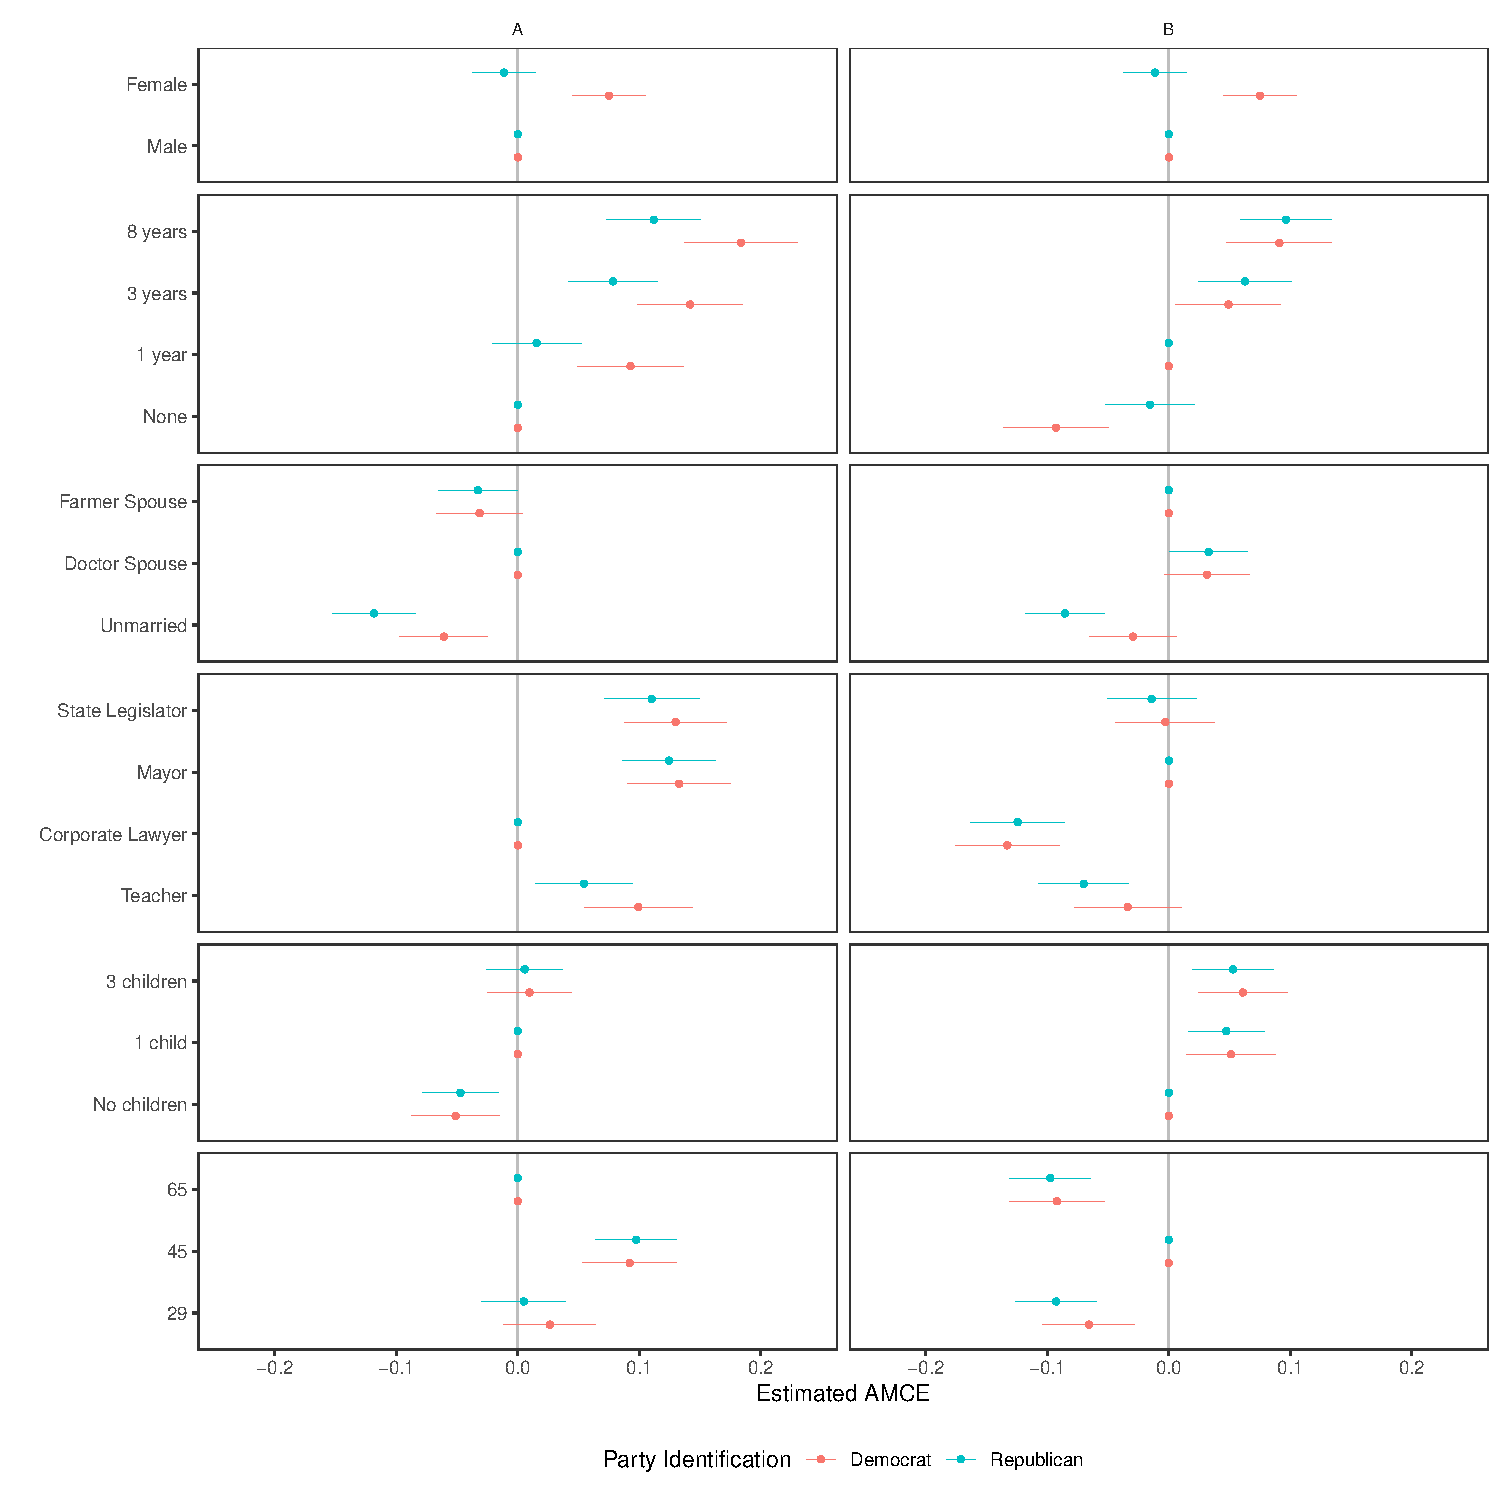
\includegraphics[width=\maxwidth]{figure/tkr_subgroup_example_plot-1} 

\end{knitrout}


\clearpage

\section*{}

\noindent This paper was built using \texttt{knitr::knit2pdf()} under the following environment:

\begin{knitrout}
\definecolor{shadecolor}{rgb}{0.969, 0.969, 0.969}\color{fgcolor}\begin{kframe}
\begin{verbatim}
## R version 3.5.3 (2019-03-11)
## Platform: x86_64-w64-mingw32/x64 (64-bit)
## Running under: Windows 7 x64 (build 7601) Service Pack 1
## 
## Matrix products: default
## 
## locale:
## [1] LC_COLLATE=English_United Kingdom.1252 
## [2] LC_CTYPE=English_United Kingdom.1252   
## [3] LC_MONETARY=English_United Kingdom.1252
## [4] LC_NUMERIC=C                           
## [5] LC_TIME=English_United Kingdom.1252    
## 
## attached base packages:
## [1] stats     graphics  grDevices utils     datasets  methods   base     
## 
## other attached packages:
## [1] gridExtra_2.3 ggplot2_3.1.1 cregg_0.3.1   rio_0.5.16   
## 
## loaded via a namespace (and not attached):
##  [1] zip_2.0.1         Rcpp_1.0.1        cellranger_1.1.0 
##  [4] pillar_1.3.1      compiler_3.5.3    plyr_1.8.4       
##  [7] forcats_0.4.0     tools_3.5.3       digest_0.6.18    
## [10] lattice_0.20-38   evaluate_0.13     tibble_2.1.1     
## [13] gtable_0.3.0      ggstance_0.3.1    pkgconfig_2.0.2  
## [16] rlang_0.3.4       Matrix_1.2-17     openxlsx_4.1.0   
## [19] curl_3.3          haven_2.1.0       xfun_0.6         
## [22] withr_2.1.2       stringr_1.4.0     knitr_1.22       
## [25] hms_0.4.2         lmtest_0.9-36     grid_3.5.3       
## [28] data.table_1.12.2 R6_2.4.0          survival_2.44-1.1
## [31] readxl_1.3.1      foreign_0.8-71    magrittr_1.5     
## [34] splines_3.5.3     scales_1.0.0      assertthat_0.2.1 
## [37] xtable_1.8-3      colorspace_1.4-1  sandwich_2.5-1   
## [40] survey_3.35-1     stringi_1.4.3     lazyeval_0.2.2   
## [43] munsell_0.5.0     crayon_1.3.4      zoo_1.8-5
\end{verbatim}
\end{kframe}
\end{knitrout}

\end{document}
